\chapter{Implemetasi}
Bab 4 menjelaskan implementasi website BlueTape dengan Framework Bootstrap 4. Pertama akan dijelaskan file apa saja yang dirubah. Kedua perubahan akses apa saja yang diubah oleh programmer untuk menjalankan website. Terakhir akan disajikan detail perubahan kode yang dijelaskan dalam kode \texttt{normal diff}.

\section{Daftar File yang Diubah dan Diganti pada Folder}
Bagian ~\ref{lst:daftarfile} menjelaskan isi file website BlueTape dan status file yang diganti dan diubah.
\begin{lstlisting}[basicstyle=\ttfamily, frame=single, caption=Perubahan isi folder BlueTape,
columns=fullflexible, keepspaces=true, breaklines=true, label={lst:daftarfile}]
.
|-- nbproject
|-- vendor
|-- www
|   |-- application
|   |   |-- cache
|   |   |-- config
|   |   |   |-- auth.php // Kode diubah
|   |   |   |-- database.php // Kode diubah
|   |   |   |-- ..dst
|   |   |-- controller
|   |   |   |-- Auth.php
|   |   |   |-- EntriJadwalDosen.php
|   |   |   |-- index.html
|   |   |   |-- LihatJadwalDosen.php
|   |   |   |-- Migrate.php
|   |   |   |-- PerubahanKuliahManage.php // Kode diubah
|   |   |   |-- PerubahanKuliahRequest.php // Kode diubah
|   |   |   |-- TranskripManage.php // Kode diubah
|   |   |   |-- TranskripRequest.php // Kode diubah
|   |   |-- core
|   |   |-- helper
|   |   |-- hooks
|   |   |-- languange
|   |   |-- libraries
|   |   |-- logs
|   |   |-- migration
|   |   |-- models
|   |   |--third_party
|   |   |--views
|   |   |   |-- auth
|   |   |   |   |-- index.html
|   |   |   |   |-- login.php // Kode diubah
|   |   |   |-- EntriJadwalDosen
|   |   |   |   |-- main.php // Kode diubah
|   |   |   |-- errors
|   |   |   |-- LihatJadwalDosen
|   |   |   |   |-- main.php // Kode diubah
|   |   |   |-- PerubahanKuliahManage
|   |   |   |   |-- email.php
|   |   |   |   |-- index.html
|   |   |   |   |-- main.php // Kode diubah
|   |   |   |   |-- printview.php
|   |   |   |-- PerubahanKuliahRequest
|   |   |   |   |-- email.php
|   |   |   |   |-- index.html
|   |   |   |   |-- main.php // Kode diubah
|   |   |   |-- templates
|   |   |   |   |-- flasmessage.php // Kode diubah
|   |   |   |   |-- head_loggedin.php // Kode diubah
|   |   |   |   |-- script_foundation.php // Kode diubah
|   |   |   |   |-- topbar_loggedin.php // Kode diubah
|   |   |   |-- TranskripManage
|   |   |   |   |-- email.php
|   |   |   |   |-- index.html
|   |   |   |   |-- main.php // Kode diubah
|   |   |   |-- TranskripRequest
|   |   |   |   |-- email.php
|   |   |   |   |-- index.html
|   |   |   |   |-- main.php // Kode diubah
|   |   |   |-- index.html
|   |   |--.htacces
|   |   |--index.html
|   |-- public
|   |   |-- fonts
|   |   |   |-- OFL.txt
|   |   |   |-- TitilliumWeb-Black.ttf
|   |   |   |-- TitilliumWeb-Bold.ttf
|   |   |   |-- TitilliumWeb-BoldItalic.ttf
|   |   |   |-- TitilliumWeb-ExtraLight.ttf
|   |   |   |-- TitilliumWeb-ExtraLightItalic.ttf
|   |   |   |-- TitilliumWeb-Italic.ttf
|   |   |   |-- TitilliumWeb-Light.ttf
|   |   |   |-- TitilliumWeb-LightItalic.ttf
|   |   |   |-- TitilliumWeb-Regular.ttf
|   |   |   |-- TitilliumWeb-SemiBold.ttf
|   |   |   |-- TitilliumWeb-SemiBoldItalic.ttf
|   |   |-- img
|   |   |   |-- logo.png // File tetap
|   |   |-- lib 
|   |   |   |-- css
|   |   |   |   |-- bootstrap.css // File baru ditambahkan
|   |   |   |   |-- bootstrap-grid.css // File baru ditambahkan
|   |   |   |   |-- bootstrap-reboot.css // File baru ditambahkan
|   |   |   |   |-- app.css 
|   |   |   |   |-- foundation.css 
|   |   |   |   |-- foundation-datetimepicker.min.css 
|   |   |   |   |-- foundation-flex.css 
|   |   |   |   |-- foundation-icon.css 
|   |   |   |   |-- foundation-icon.eot 
|   |   |   |   |-- foundation-icon.svg 
|   |   |   |   |-- foundation-icon.ttf 
|   |   |   |   |-- foundation-icon.woff 
|   |   |   |-- fontawesome
|   |   |   |   |-- fontawesome.css // File baru ditambahkan
|   |   |   |-- jquery
|   |   |   |   |--jquery-3.4.1.min.js // File baru ditambahkan
|   |   |   |-- js
|   |   |   |   |-- bootstrap.js // File baru ditambahkan
|   |   |   |   |-- bootstrap.bundle.js // File baru ditambahkan
|   |   |   |   |-- vendor // Folder dihapus
|   |   |   |   |-- app.js // Folder dihapus
|   |   |   |   |-- foundation.js // Folder dihapus
|   |   |   |-- xdan-datetimepicker 
|   |   |   |   |-- jquery.datetimepicker.full.min.js
|   |   |   |   |-- jquery.datetimepicker.min.js
|   |   |   |   |-- jquery.datetimepicker.min.js
|   |   |-- webfonts // Folder ditambahkan, berfungsi untuk simpan ikon.
|   |-- system
|   |-- .htaccess
|   |-- .composer.json
|   |-- .contributig.md
|   |-- .index.php
|   |-- .licence.txt
|   |-- readme.rst
|   |-- web.config
.
\end{lstlisting}

\section{Pengaturan Akses bagi \textit{admin}}
Sebelumm menjalankan website, \textit{admin} akan menyunting email admin dan database agar lebih mudah untuk diakses. Hasil perubahan kode ditampilkan dalam berbentuk diff, dimana bagian berwarna merah merupakan kode lampau(Foundation 6) dan bagian berwarna hijau merupakan kode terkini  (Bootstrap 4).

\subsection{Perubahan Akses URL}
Saat admin pertama kali menjalankan aplikasi CodeIgniter maka diperlukan konfigurasi \texttt{base\_url}. Sehingga URL baru terbentuk dan dapat mengakses \textit{resource} yang ada pada direktori \texttt{root}. Penggunaan \texttt{base\_url} dalam website dijelaskan pada kode ~\ref{lst:config}\\

\begin{lstlisting}[language=diff, caption=Perubahan file /config/config.php,  basicstyle=\ttfamily, frame=single,
columns=fullflexible, keepspaces=true, breaklines=true, label={lst:config}]
diff -r a\www\application\config\config.php b\www\application\config\config.php

26c26
< $config['base_url'] = 'https://bluetape.azurewebsites.net';
---
> $config['base_url'] = 'http://127.0.0.1/';
\end{lstlisting}

\subsection{Perubahan Akses Email Admin}

Kode ~\ref{lst:modules} mengarahkan admin ke halaman login setelah aplikasi berjalan, karena website menggunakan \textit{Google API Console} untuk proses autentikasi maka perlu ditambahkan email admin baru pada file \path{www/application/config/modules.php}. Email ini telah didaftarkan sebelumnya di API tersebut, sehingga admin dapat menggunakan seluruh fitur pada website. \\

\begin{lstlisting}[language=diff, caption=Perubahan file /config/modules.php,  basicstyle=\ttfamily, frame=single,
columns=fullflexible, keepspaces=true, breaklines=true, label={lst:modules}]
diff -r a\www\application\config\modules.php 	b\www\application\config\modules.php
25,26c25,26
<     'root' => array('pascal@unpar.ac.id', 'shao.wei@unpar.ac.id'),
<     'tu.ftis' => array('shao.wei@unpar.ac.id', 'purnomo@unpar.ac.id', 'walip@unpar.ac.id'),
---
>     'root' => array('pascal@unpar.ac.id', 'shao.wei@unpar.ac.id', 'amihapsahapsa@gmail.com'),
>     'tu.ftis' => array('shao.wei@unpar.ac.id', 'pranyoto@unpar.ac.id', 'walip@unpar.ac.id'),

\end{lstlisting}

\section{Perubahan Kode pada Tampilan}

Bagian ini akan menjelaskan hasil implementasi dalam bentuk \textit{diff}. Diff membedakan kode berdasarkan warna dimana bagian berwarna merah merupakan kode lampau(implementasi dengan Foundation 6) dan bagian berwarna hijau merupakan kode terkini  (implementasi dengan Bootstrap 4).

\subsection{Penggunaan \textit{library} Bootstrap 4 pada Website}

Library Bootstrap 4 yang sudah dimasukan pada CodeIgniter akan diintegrasikan pada file www/application/config/modules.php dalam bentuk file \texttt{.js} dan \texttt{head\_loggedin.php} dalam bentuk file \texttt{.css}. File ini nantinya akan dipakai keseluruh halaman website kecuali halaman login.\\

Pertama kode ~\ref{lst:scriptfoundation} memanggil file js dan jquery untuk Bootstrap serta plugin \texttt{xdan-datetimepicker} agar dapat di\textit{load}. \\

\begin{lstlisting}[language=diff, caption=Penambahan \path{\views\templates\script_foundation.php},  basicstyle=\ttfamily, frame=single,
columns=fullflexible, keepspaces=true, breaklines=true, label={lst:scriptfoundation}]
diff -r a\www\application\views\templates\script_foundation.php b\www\application\views\templates\script_foundation.php
3,6c3,4
< ?><script src="/public/js/vendor/jquery.min.js"></script>
< <script src="/public/js/vendor/what-input.min.js"></script>
< <script src="/public/js/foundation.min.js"></script>
< <script src="/public/js/app.js"></script>
---
> ?><script src="/public/lib/jquery/jquery-3.4.1.min.js"></script>
> <script src="/public/lib/js/bootstrap.js"></script>

\end{lstlisting}

Kedua file css akan dipanggil, ada tiga macam file yang dipanggil: 
\begin{itemize}
	\item \textit{library} Bootstrap 4.
	\item Plugin \texttt{xdan-datetimepicker}.
	\item \textit{library} Font Awesome.
\end{itemize}
File yang berisi kode ~\ref{lst:headloggedin} akan digunakan pada seluruh halaman website kecuali halaman login.

\begin{lstlisting}[language=diff, caption=Perubahan file \path{\views\templates\head_loggedin.php},  basicstyle=\ttfamily, frame=single,
columns=fullflexible, keepspaces=true, breaklines=true, label={lst:headloggedin}]
diff -r a\www\application\views\templates\head_loggedin.php b\www\application\views\templates\head_loggedin.php
8,11c8,10
<     <link rel="stylesheet" href="/public/css/foundation.css" />
<     <link rel="stylesheet" href="/public/css/foundation-icons.css" />
<     <link rel="stylesheet" href="/public/css/app.css" />
<     <link rel="stylesheet" href="/public/lib/xdan-datetimepicker/jquery.datetimepicker.min.css" />
---
>     <link rel="stylesheet" href="/public/lib/css/bootstrap.css" />
>     <link rel="stylesheet" href="/public/lib/fontawesome/fontawesome.css">
>     <link rel="stylesheet" href="public/lib/xdan-datetimepicker/jquery.datetimepicker.min.css">

\end{lstlisting}

\subsection{Halaman Login}
\noindent Gambar ~\ref{fig:analisisLogin} adalah halaman pertama yang diakses \textit{user}, penjelasan untuk setiap tombol yang ada direferensikan pada ~\ref{ss:login}.

\begin{figure} [H]
	\centering  	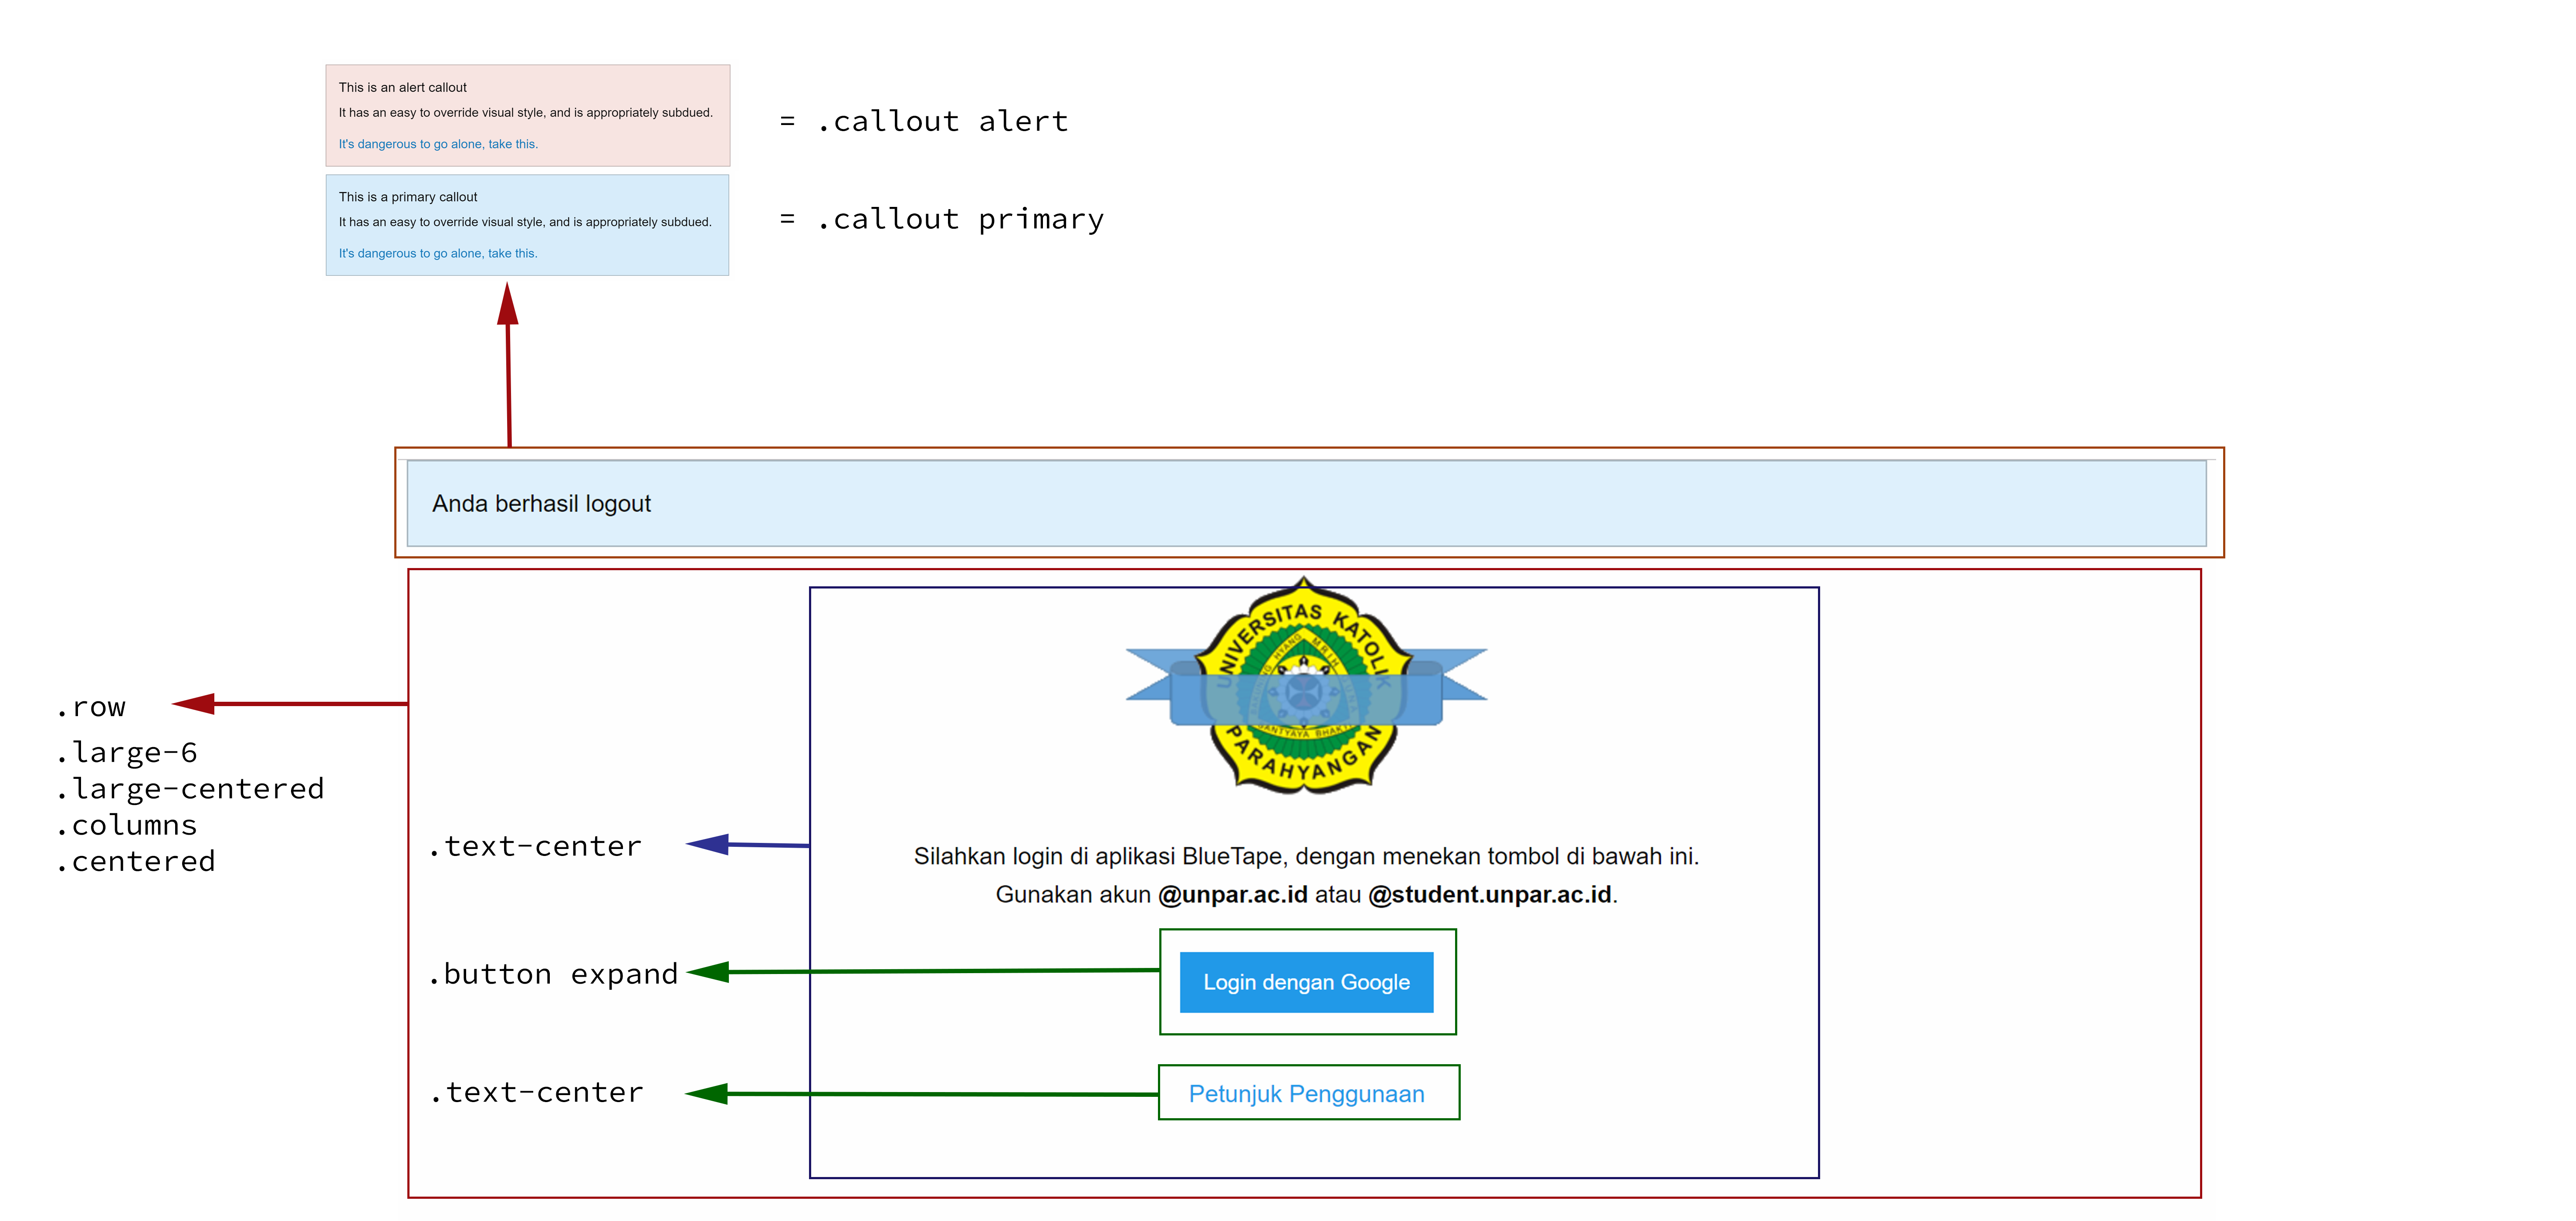
\includegraphics[width=\textwidth,height=\textheight,keepaspectratio]{foundation/analisis_login.png} 
	\caption{Halaman login dengan Foundation 6.} 
	\label{fig:analisisLogin}
\end{figure}

\noindent Gambar ~\ref{fig:konversiLogin} menjelaskan komponen dalam website beserta penamaan kelas untuk Bootstrap 4 pada halaman login.\\
\begin{figure} [H]
	\centering  
	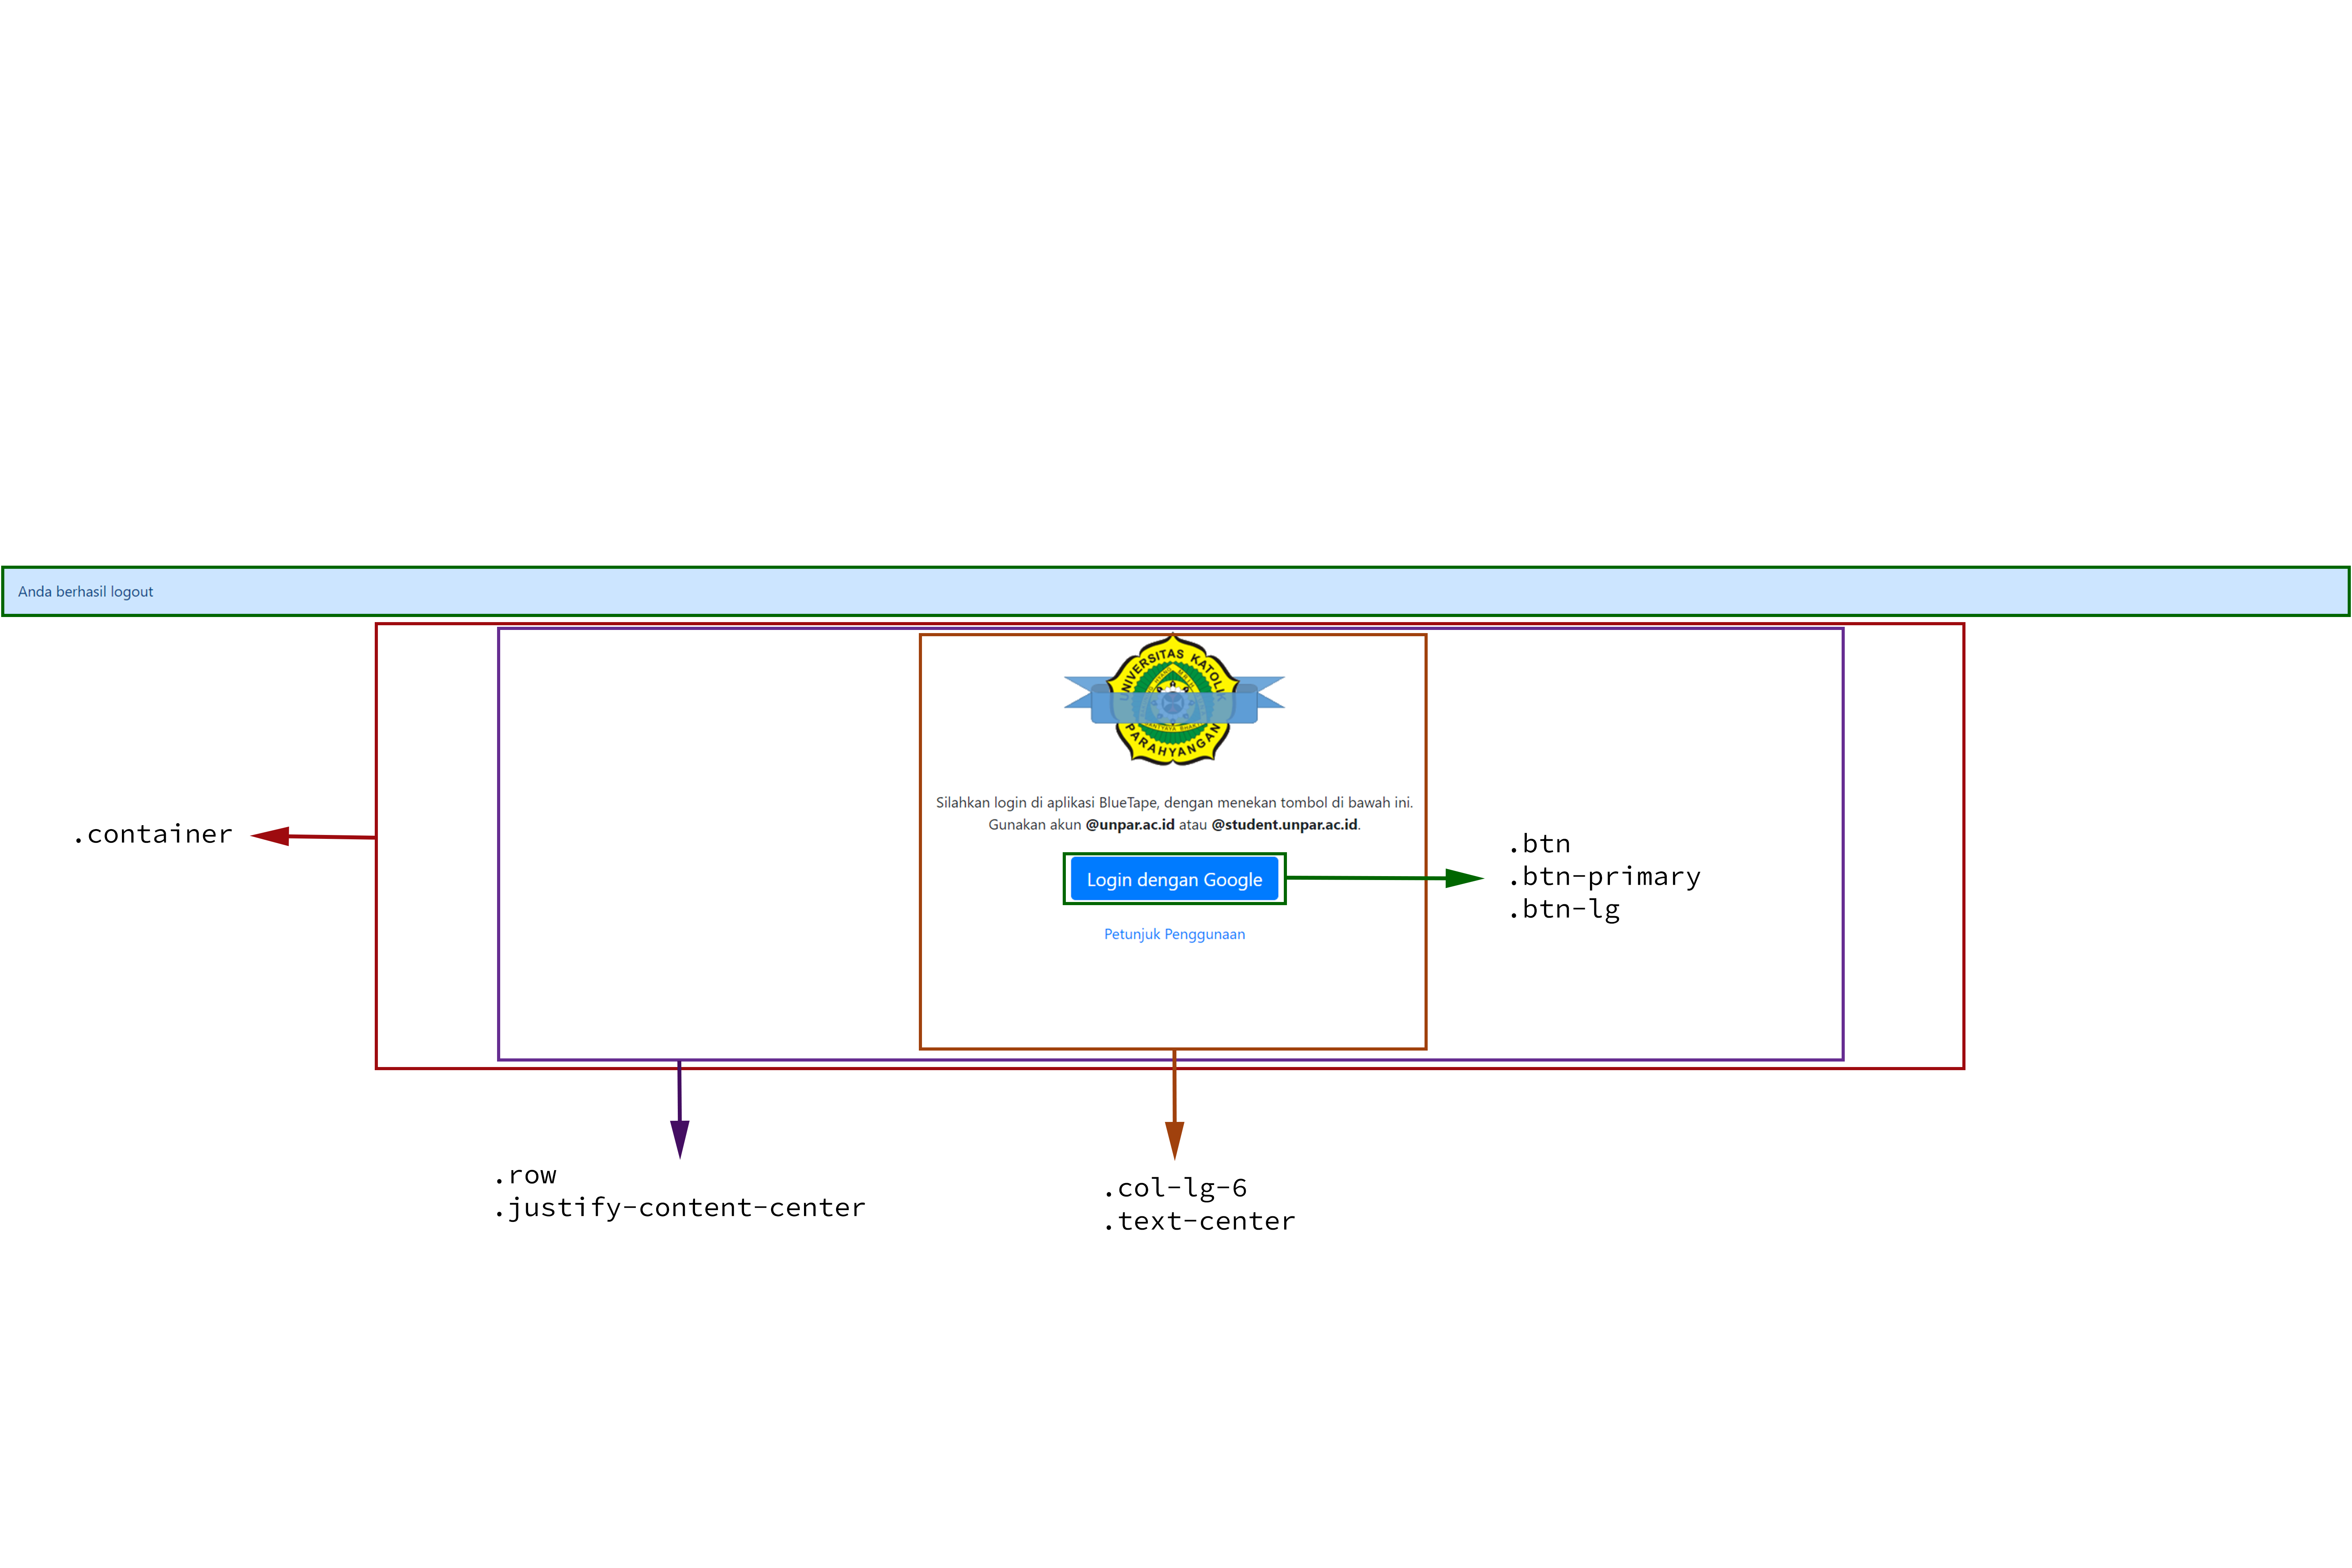
\includegraphics[width=\textwidth,height=\textheight,keepaspectratio]{bootstrap/konversi_tampilan_login.png}  
	\caption{Halaman login dengan Bootstrap 4.} 
	\label{fig:konversiLogin}
\end{figure} \noindent \\

Pemanggilan file css untuk \textit{framework} dilakukan pada file \texttt{login.php} yang terlihat pada kode ~\ref{lst:login}. Kemudian terdapat kode HTML untuk halaman login.
\begin{lstlisting}[language=diff, caption=Perubahan file \path{\views\auth\login.php},  basicstyle=\ttfamily, frame=single,
columns=fullflexible, keepspaces=true, breaklines=true, label={lst:login}]
diff -r a\www\application\views\auth\login.php b\www\application\views\auth\login.php
10,11c10,13
< <link rel="stylesheet" href="/public/css/foundation.css" />
< <link rel="stylesheet" href="/public/css/app.css" />
---
> <link rel="stylesheet" href="/public/lib/css/bootstrap.css" />
> <link rel="stylesheet" href="/public/lib/css/bootstrap-grid.css" />
> <link rel="stylesheet" href="/public/lib/css/bootstrap-reboot.css" />
> <link rel="stylesheet" href="/public/lib/fontawesome/fontawesome.css" />

15,16c17,19
< <div class="row">
<     <div class="large-6 large-centered columns centered">
---
> <div class="container">
>     <div class="row justify-content-center">
>         <div class="col-lg-6">

21,22c24,25
< <a href="<?= $authURL; ?>" class="button expand">Login dengan Google</a><br/><br/>
< <a class="text-center" href="https://github.com/ftisunpar/BlueTape/wiki/UserGuide" target="_blank">Petunjuk Penggunaan</a>
---
> <a href="<?= $authURL; ?>" class="btn btn-primary btn-lg">Login dengan Google</a><br/><br/>
> <a href="https://github.com/ftisunpar/BlueTape/wiki/UserGuide" target="_blank">Petunjuk Penggunaan</a>
\end{lstlisting}
Kode lengkap dari file ini dapat dilihat dalam lampiran ~\ref{lst:reslogin}.

\noindent Penjelasan kode diatas tertera pada tabel ~\ref{table:KodeManajemenPerubahanKuliah}:
\begin{table}[H]
	\centering
	\caption{Penjelasan kode konversi halaman manajemen perubahan kuliah.}
	\begin{tabularx}{\textwidth}{llX}
		\toprule
		No Line & Implementasi     & Penjelasan \\
		\midrule
		2 & \textbf{Pemanggilan file} & File css dari Foundation akan diganti dengan file css dari Bootstrap 4.\\
		12, 15 & \textbf{Grid konten} & Dalam Foundation 6 untuk membuat satu baris konten hanya menggunakan kelas \texttt{.row}, namun di Bootstrap 4 perlu ditambahakan kelas \texttt{.container}.\\
		& & Untuk size sama - sama menggunakan lebar 6 grid yang posisi nya diletakkan ditengah website.\\
		21, 24 & \textbf{Text} & Teks akan diletakkan ditengah, hanya di Foundation 6 saja perlu menginisiasi kelas \texttt{.text-center} pada Bootstrap 4 tidak perlu.\\
		\bottomrule
	\end{tabularx}%
	\label{table:KodeManajemenPerubahanKuliah}
\end{table}

Implementasi notifikasi user terdapat pada kode ~\ref{lst:flashmessage}.

\begin{lstlisting}[language=diff, caption=Perubahan file \path{\views\templates\flashmessage.php},  basicstyle=\ttfamily, frame=single,
columns=fullflexible, keepspaces=true, breaklines=true, label={lst:flashmessage}]
diff -r a\www\application\views\templates\flashmessage.php b\www\application\views\templates\flashmessage.php

5c5
< <div class="callout alert"><?= $_SESSION['error'] ?></div>
---
> <div class="alert alert-danger" role="alert"><?= $_SESSION['error'] ?></div>

8c8
< <div class="callout primary"><?= $_SESSION['info'] ?></div>
---
> <div class="alert alert-primary" role="alert"><?= $_SESSION['info'] ?></div>
\end{lstlisting}

\noindent Beberapa catatan dari kode diatas berada pada tabel ~\ref{tabelKodeLogin}:

\begin{table}[H]
	\centering
	\caption{Penjelasan kode konversi halaman login.}
	\begin{tabularx}{\textwidth}{llX}
		\toprule
		No Line & Implementasi     & Penjelasan \\
		\midrule
		9, 11 & \textbf{Alert} & Labelling menggunakan \texttt{.callout} pada Foundation 6. Boostrap 4 mrnggunakan kelas \texttt{.alert} dan atribut \texttt{role}.\\
		\bottomrule
	\end{tabularx}%
	\label{tabelKodeLogin}
\end{table}

\subsection{Menu Navigasi}
Komponen menu navigasi digunakan pada keseluruhan tampilan website, bentuk menu akan menyesuaikan sesuai dengan layar dimana website diakses. \\
Berikut ini gambar ~\ref{fig:navigasiLarge} merupakan hasil penggunaan dari implementasi menu navigasi:

\begin{figure} [H]
	\centering  
	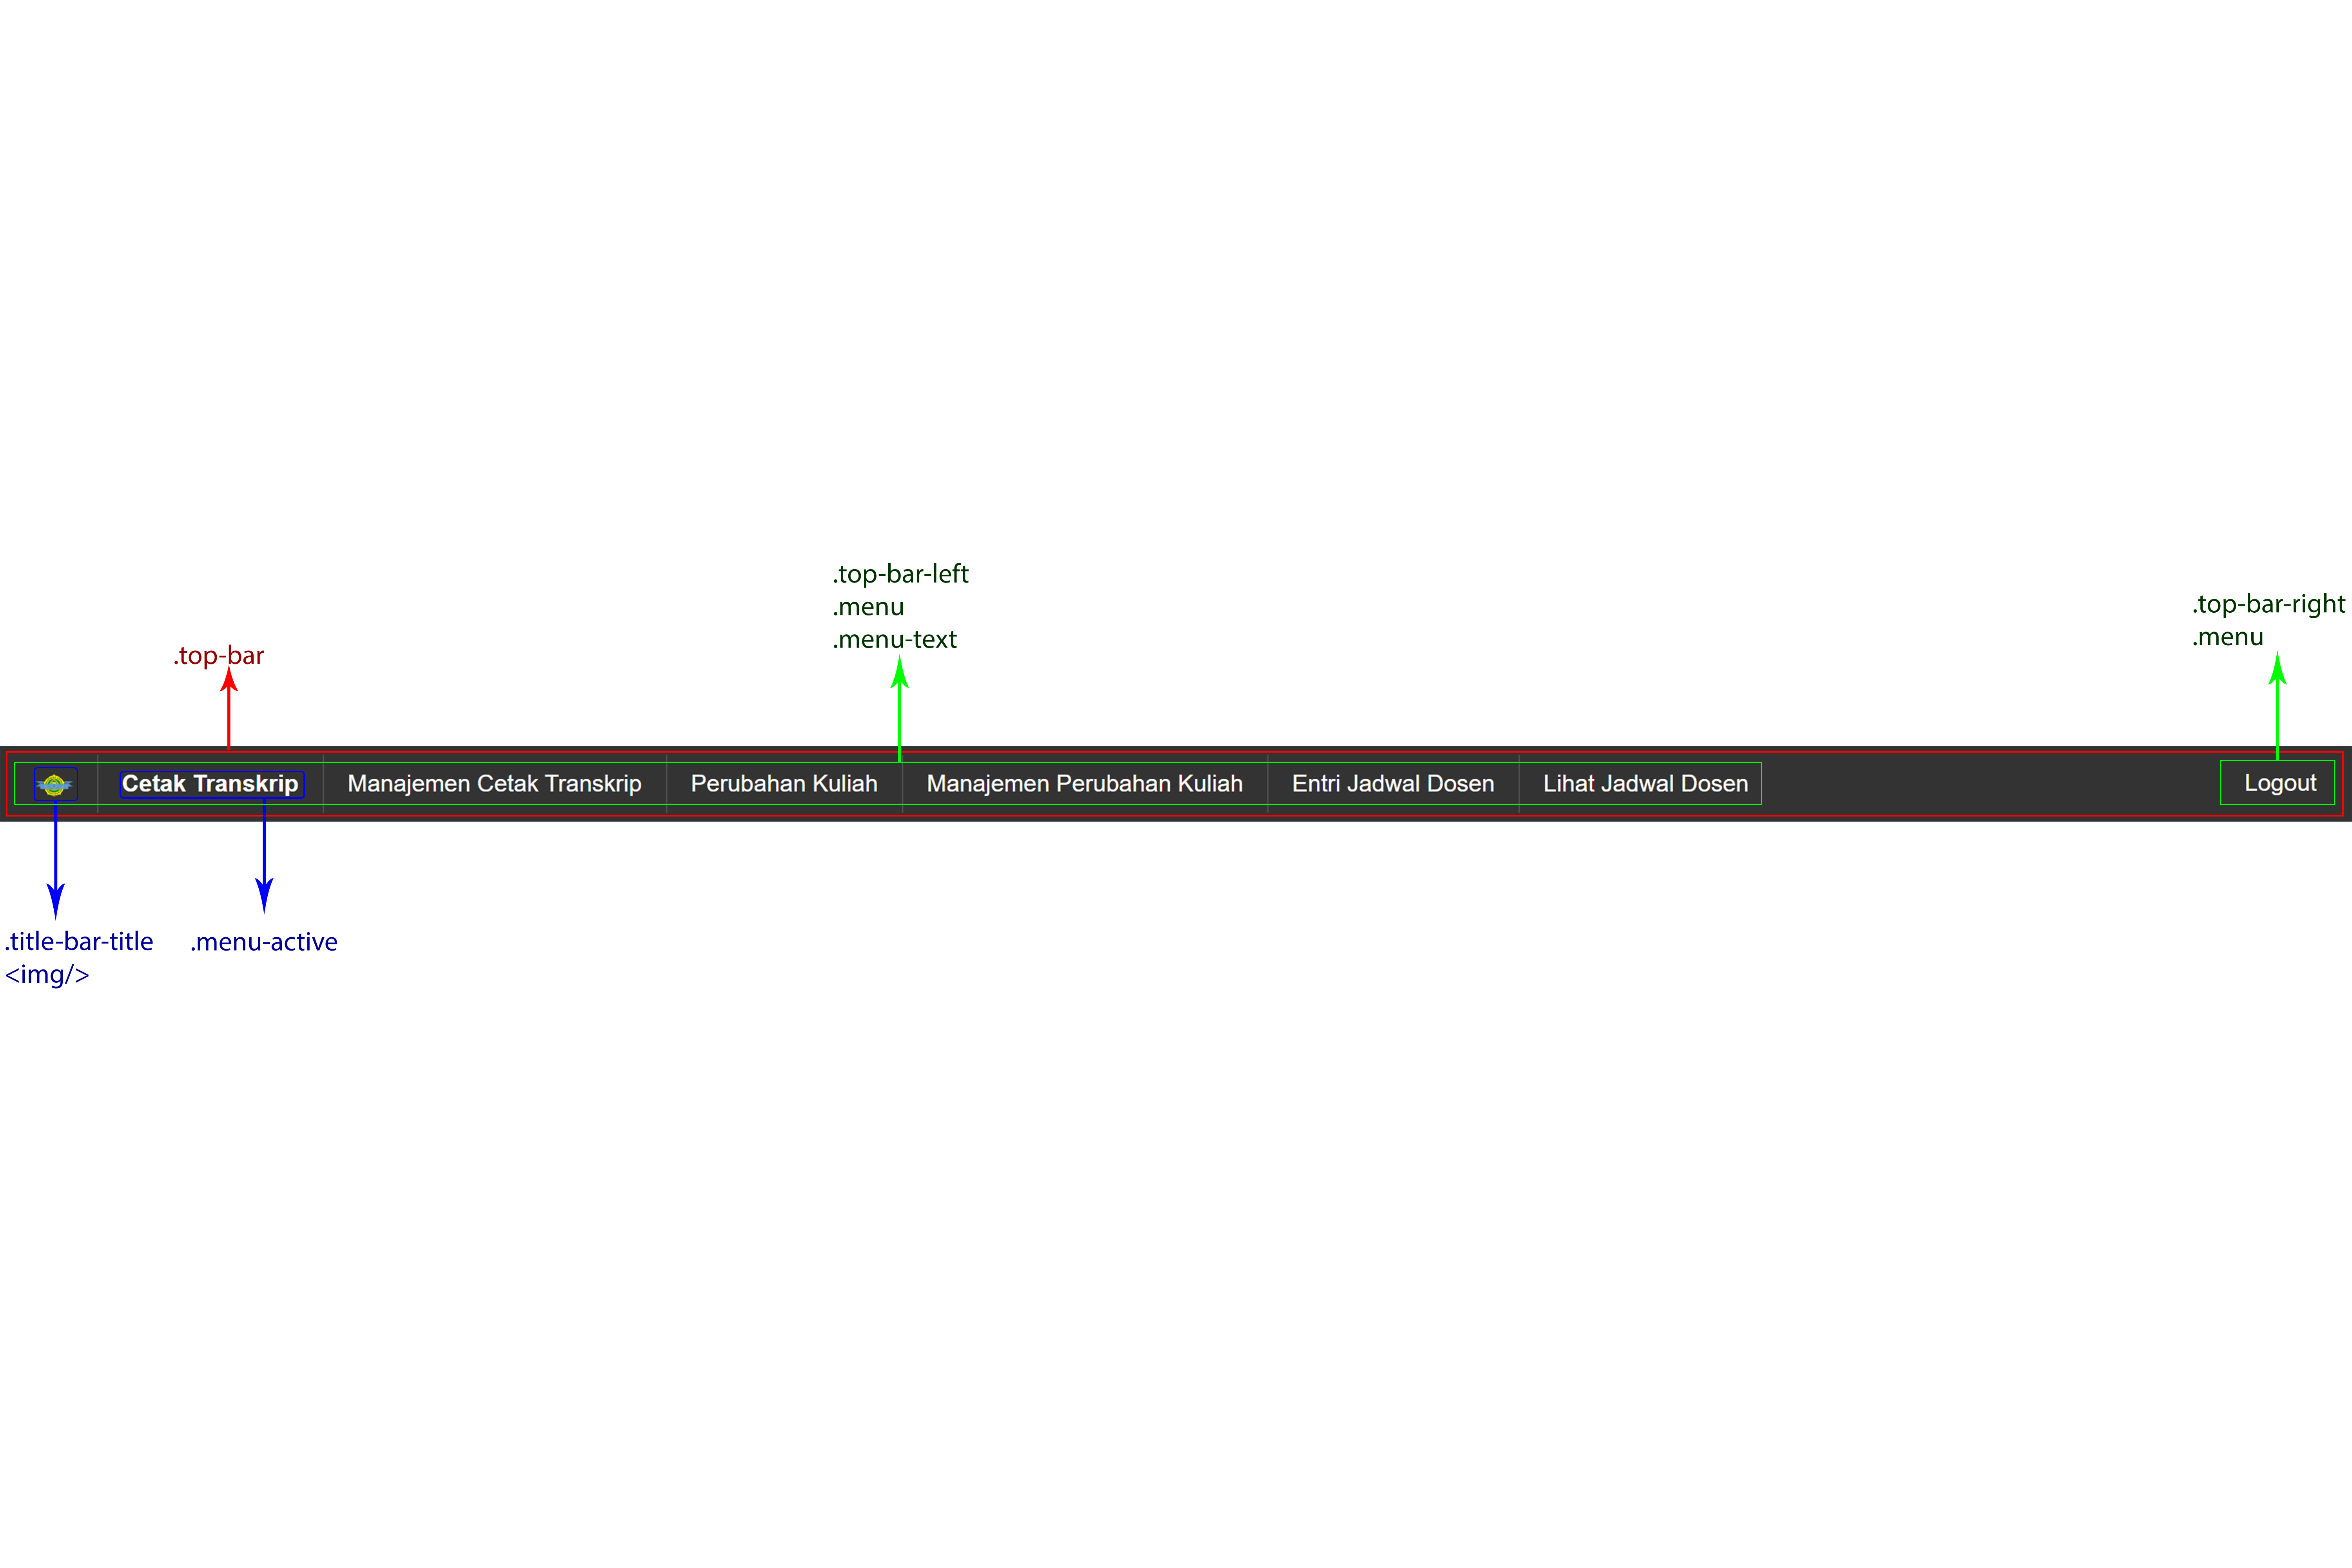
\includegraphics[width=\textwidth,height=\textheight,keepaspectratio]{foundation/analisis_top_bar.png}  
	\caption{Analisis menu navigasi di layar \textit{large}.} 
	\label{fig:navigasiLarge}
\end{figure}

\noindent Gambar ~\ref{fig:konversiNavigasi} menjelaskan komponen dalam website beserta penamaan kelas untuk Bootstrap 4 pada menu navigasi.\\
\begin{figure} [H]
	\centering  
	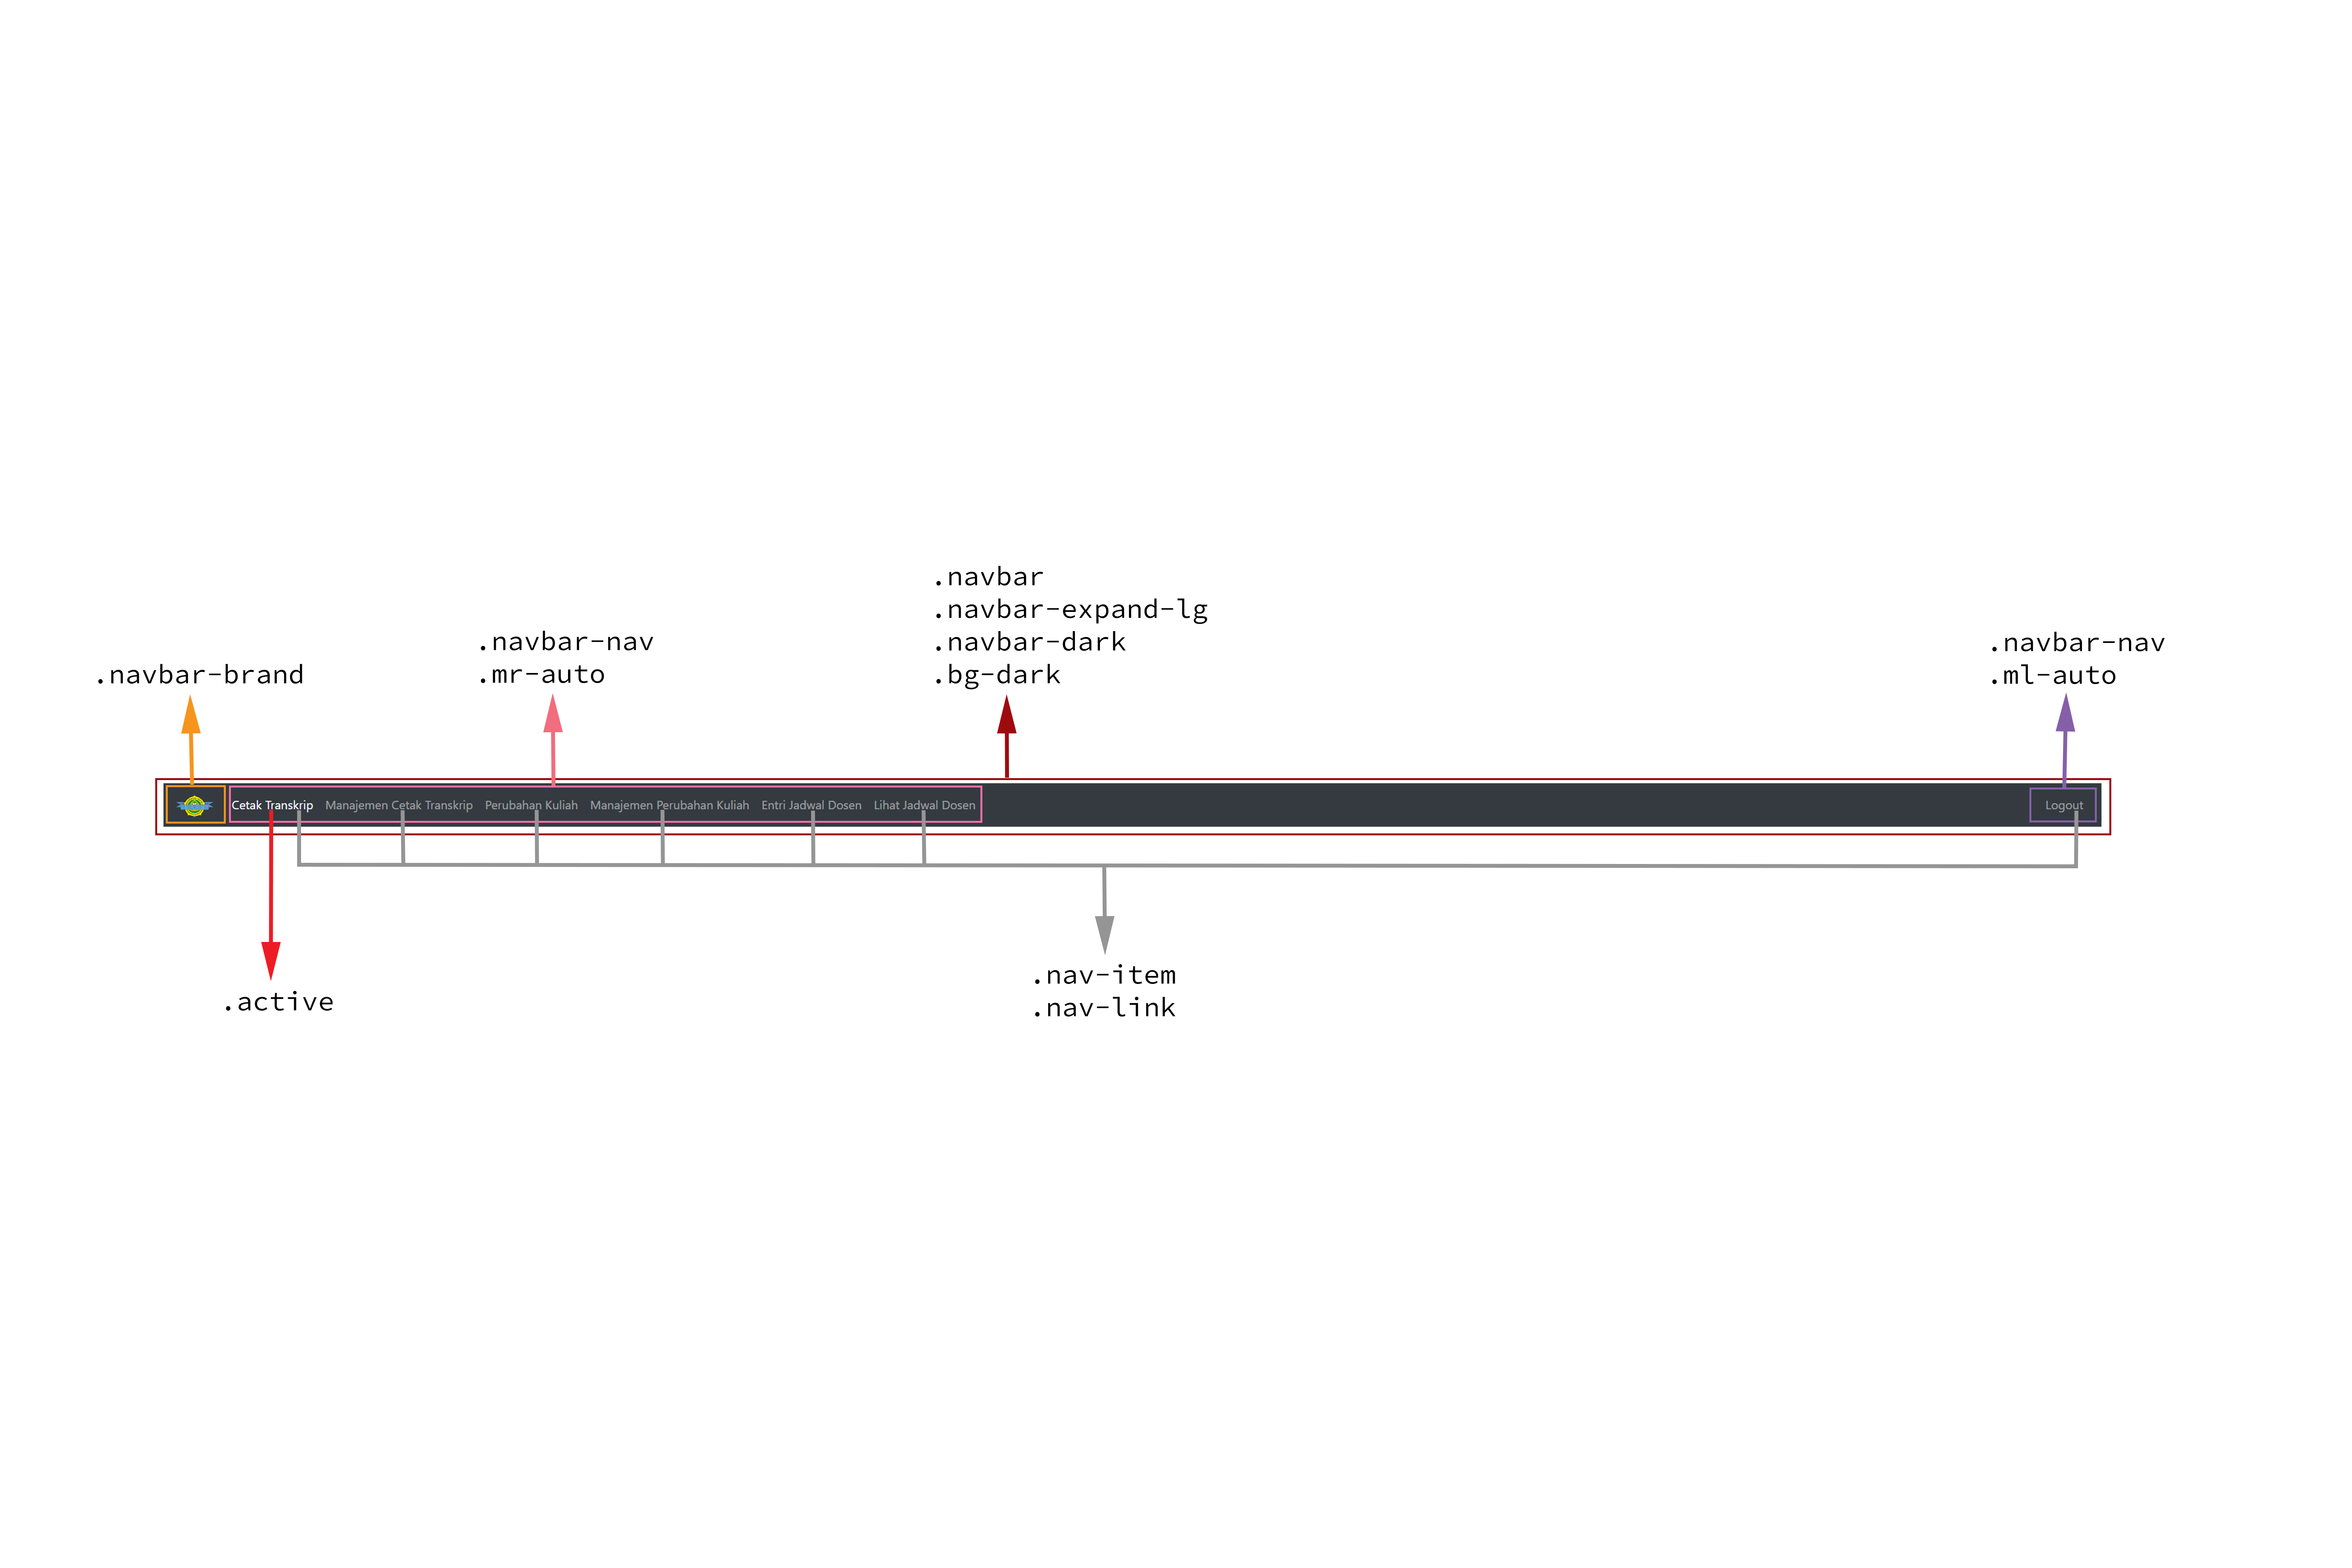
\includegraphics[width=\textwidth,height=\textheight,keepaspectratio]{bootstrap/konversi_navbar.png}  
	\caption{Konversi menu navigasi di layar \textit{large}.} 
	\label{fig:konversiNavigasi}
\end{figure}

\noindent Lalu untuk layar \textit{medium} dan \textit{small} menggunakan komponen \texttt{Advanced Layout} pada gambar ~\ref{fig:navigasiMedium} dimana  daftar halaman website yang ada pada menu berada di mode \textit{hide} dan digantian oleh ikon menu. 

\begin{figure} [H]
	\centering  
	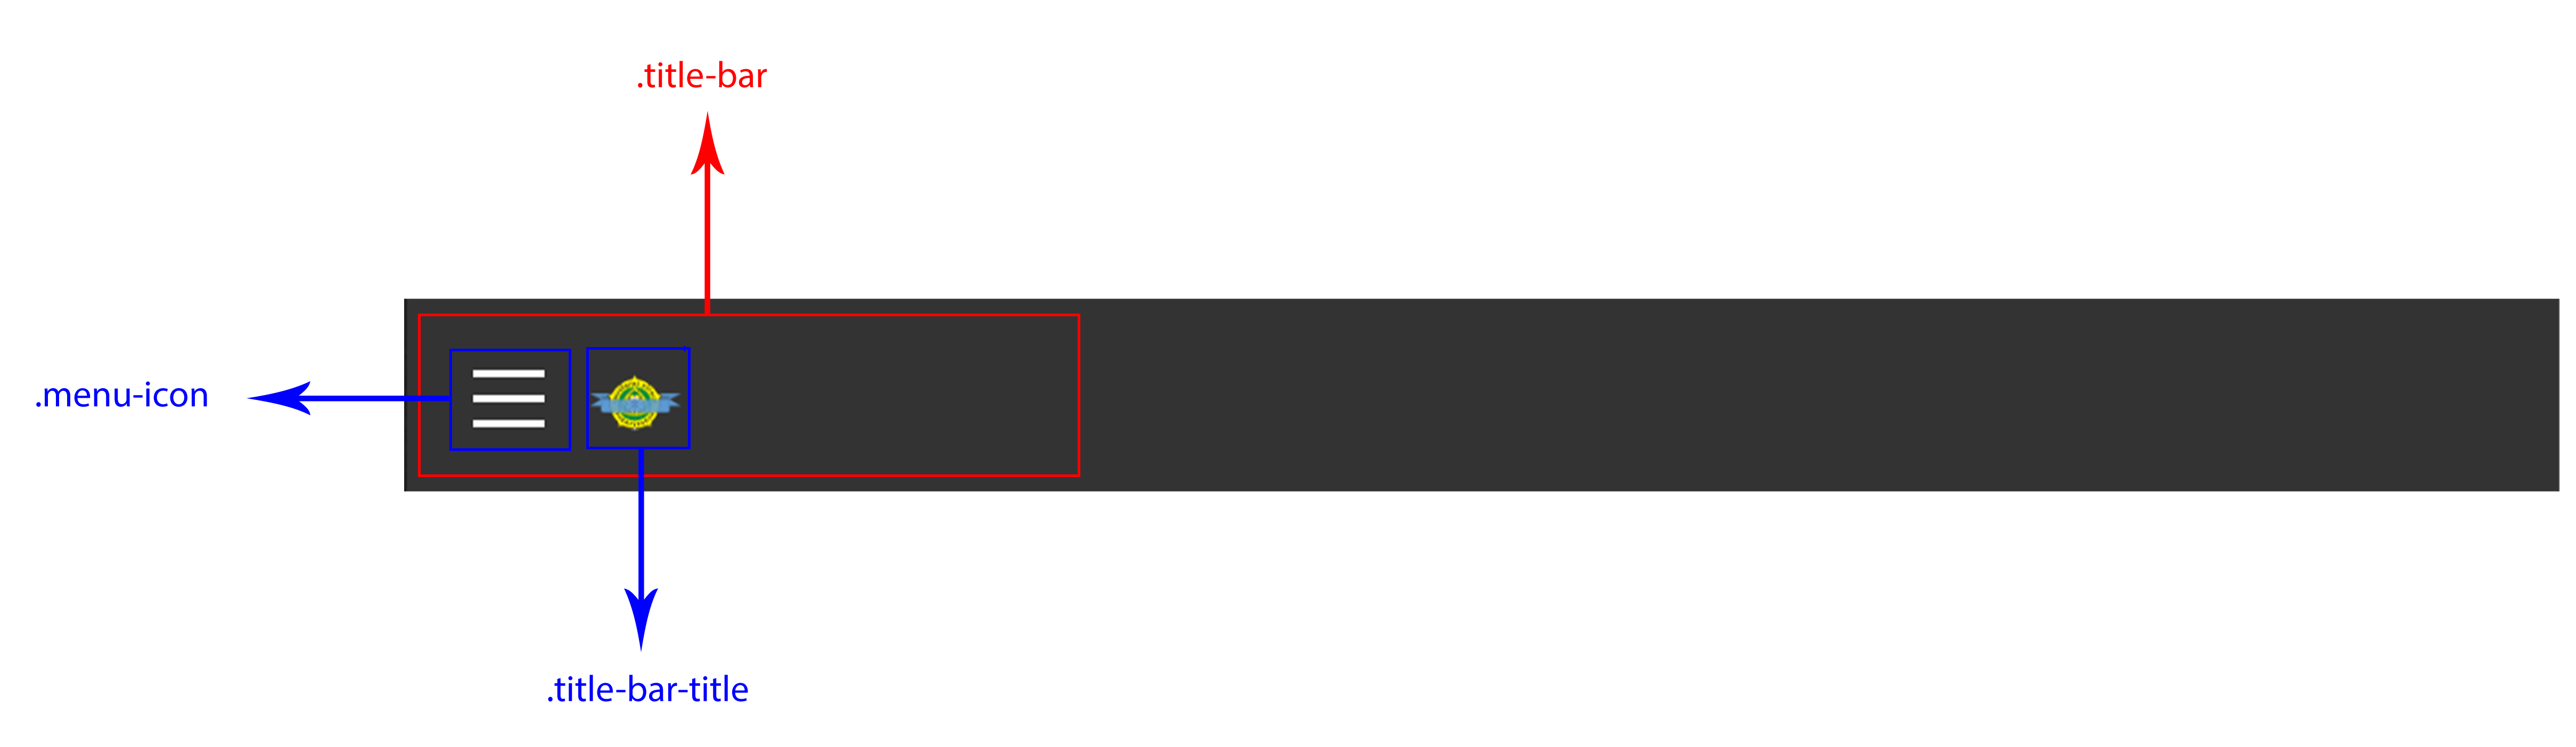
\includegraphics[width=\textwidth,height=\textheight,keepaspectratio]{foundation/analisis_top_bar_small.png} 
	\caption{Analisis menu navigasi di layar \textit{medium} dan \textit{small}.} 
	\label{fig:navFoundation}
\end{figure} \noindent
\begin{figure} [H]
	\centering  
	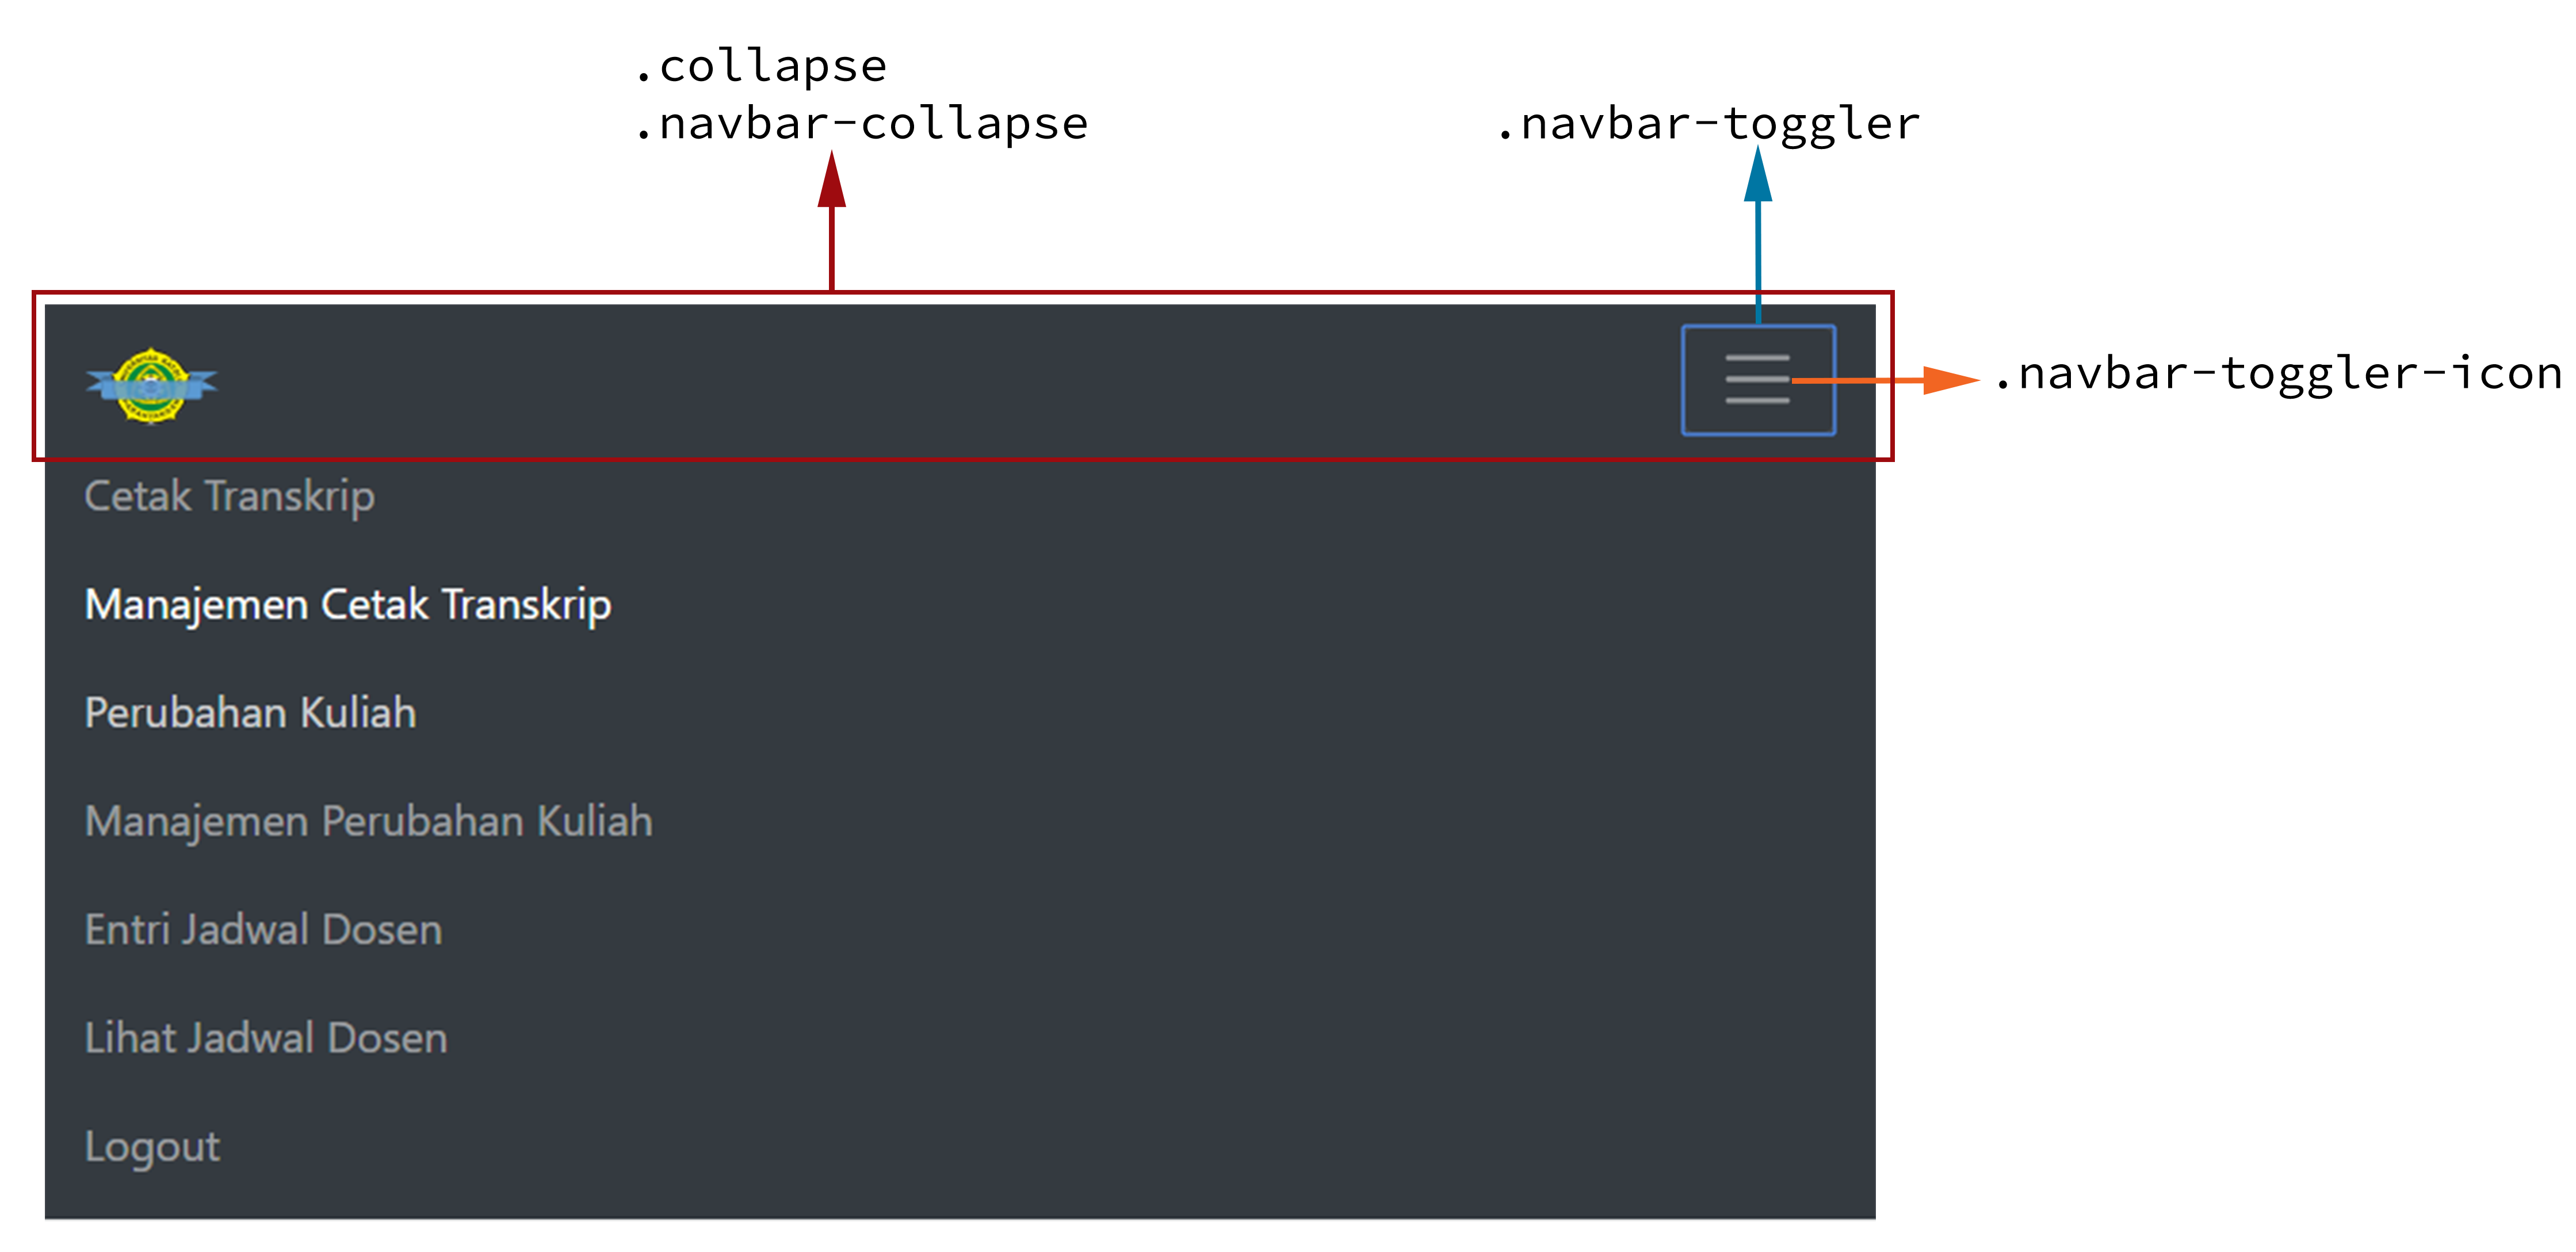
\includegraphics[width=\textwidth,height=\textheight,keepaspectratio]{bootstrap/konversi_small_navbar.png} 
	\caption{Konversi menu navigasi di layar \textit{medium} dan \textit{small}.} 
	\label{fig:navBootstrap}
\end{figure} \noindent


Kode ~\ref{lst:topbarloggedin} menjelaskan menu navigasi secara umum terdiri dari kelas untuk judul website, letak menu dan menu yang sedang aktif.
\begin{lstlisting}[language=diff, caption=Perubahan file \path{\views\templates\topbar_loggedin.php} ,  basicstyle=\ttfamily, frame=single,
columns=fullflexible, keepspaces=true, breaklines=true, label={lst:topbarloggedin}]
diff -r a\www\application\views\templates\topbar_loggedin.php b\www\application\views\templates\topbar_loggedin.php

3,11c3,12
< ?><div class="title-bar" data-responsive-toggle="navigation-menu" data-hide-for="medium">
<     <button class="menu-icon" type="button" data-toggle></button>
<     <div class="title-bar-title"><img src="/public/img/logo.png" class="textsized" alt="B"/></div>
< </div>
< 
< <div class="top-bar" id="navigation-menu">
<     <div class="top-bar-left">
<         <ul class="menu" data-responsive-menu="dropdown">
<             <li class="menu-text"><img src="/public/img/logo.png" class="textsized" alt="B"/></li>
---
> ?>
> 
> <nav class="navbar navbar-expand-lg navbar-dark bg-dark">
>     <a class="navbar-brand" href="#"><img src="/public/img/logo.png" width="50"/></a>
>     <button class="navbar-toggler" type="button" data-toggle="collapse" data-target="#navbarSupportedContent" aria-controls="navbarSupportedContent" aria-expanded="false" aria-label="Toggle navigation">
>         <span class="navbar-toggler-icon"></span>
>     </button>
> 
>     <div class="collapse navbar-collapse" id="navbarSupportedContent">
>         <ul class="navbar-nav mr-auto">

13c14
< <li<?= $module === $currentModule ? ' class="menu-active"' : '' ?>><a href="/<?= $module ?>"><?= $this->config->item('module-names')[$module] ?></a></li>
---
> <li <?= $module == $currentModule ? ' class="nav-item active"' : ' class="nav-item "' ?>><a class="nav-link" href="/<?= $module ?>"><?= $this->config->item('module-names')[$module] ?></a></li>

16,19c17,20
< </div>
< <div class="top-bar-right">
< 	<ul class="menu">
< 	    <li><a href="/auth/logout">Logout</a></li>
---
> <ul class="navbar-nav ml-auto">
>     <li class="nav-item">
>         <a class="nav-link" href="/auth/logout">Logout</a>
>     </li>
\end{lstlisting}

\noindent Catatan untuk kode ~\ref{lst:topbarloggedin} dijabarkan dalam tabel ~\ref{tabel:KodeLogin}:
\begin{table}[H]
	\centering
	\caption{Penjelasan kode konversi navigasi bar.}
	\begin{tabularx}{\textwidth}{llX}
		\toprule
		No Line & Implementasi     & Penjelasan \\
		\midrule
		3-39 & \textbf{Navbar} & Pada foundation 6 ikon dropdown belum berfungsi, sehingga pada Bootstrap 4 menu dibuat \textit{responsive} sehingga terdapat ikon yang menyimpan daftar menu.\\
		\bottomrule
	\end{tabularx}%
	\label{tabel:KodeLogin}
\end{table}

\subsection{Halaman Permintaan Cetak Transkrip }
Berikut ini gambar ~\ref{fig:analisisCetakTranskrip} merupakan hasil implementasi permintaan cetak transkrip:
\begin{figure} [H]
	\centering  
	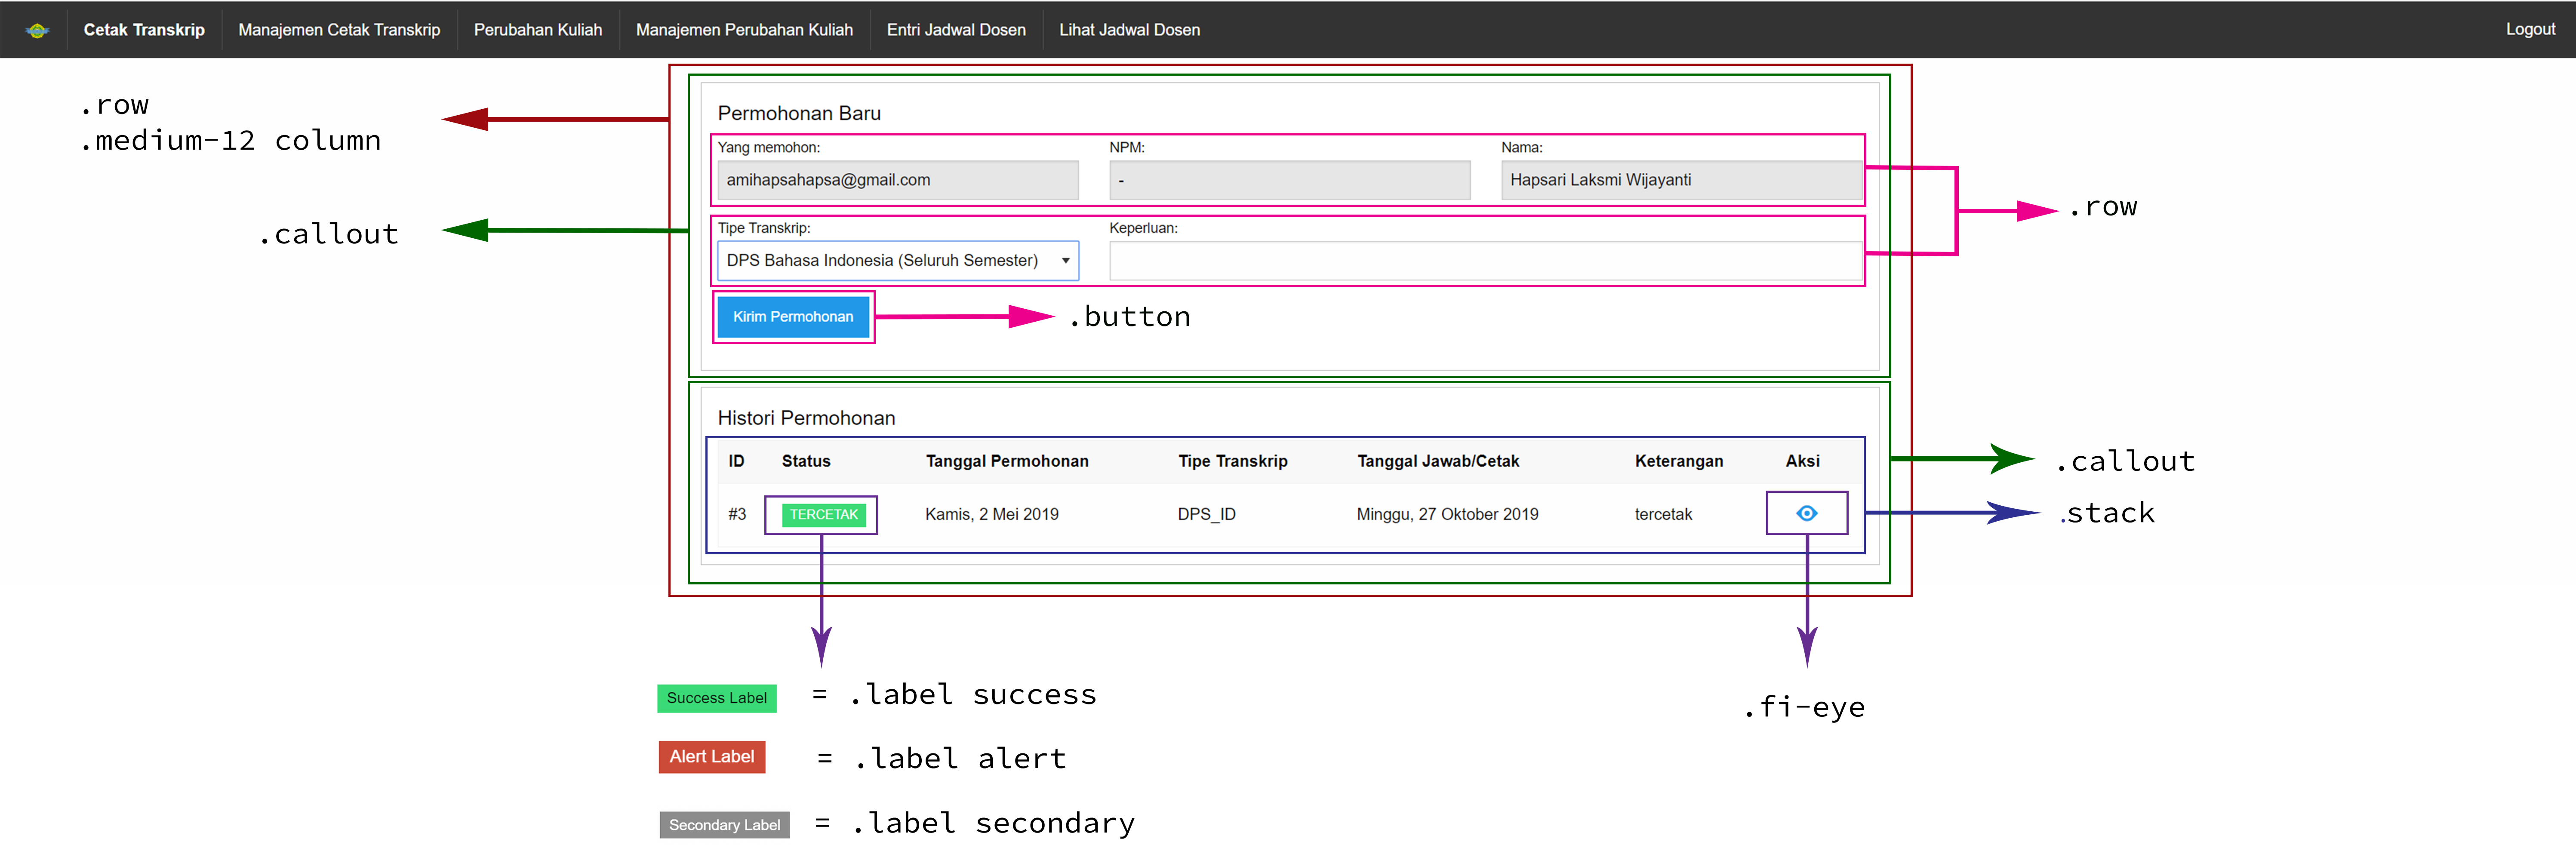
\includegraphics[width=\textwidth,height=\textheight,keepaspectratio]{foundation/analisis_mahasiswa_cetak_transkrip.png}
	\caption{Analisis halaman cetak transkrip.} 
	\label{fig:analisisCetakTranskrip}
\end{figure} 

\noindent Gambar ~\ref{fig:konversiPermintaanCetakTranskrip} menjelaskan komponen dalam website beserta penamaan kelas untuk Bootstrap 4 pada halaman permintaan cetak transkrip.\\

\begin{figure} [H]
	\centering  
	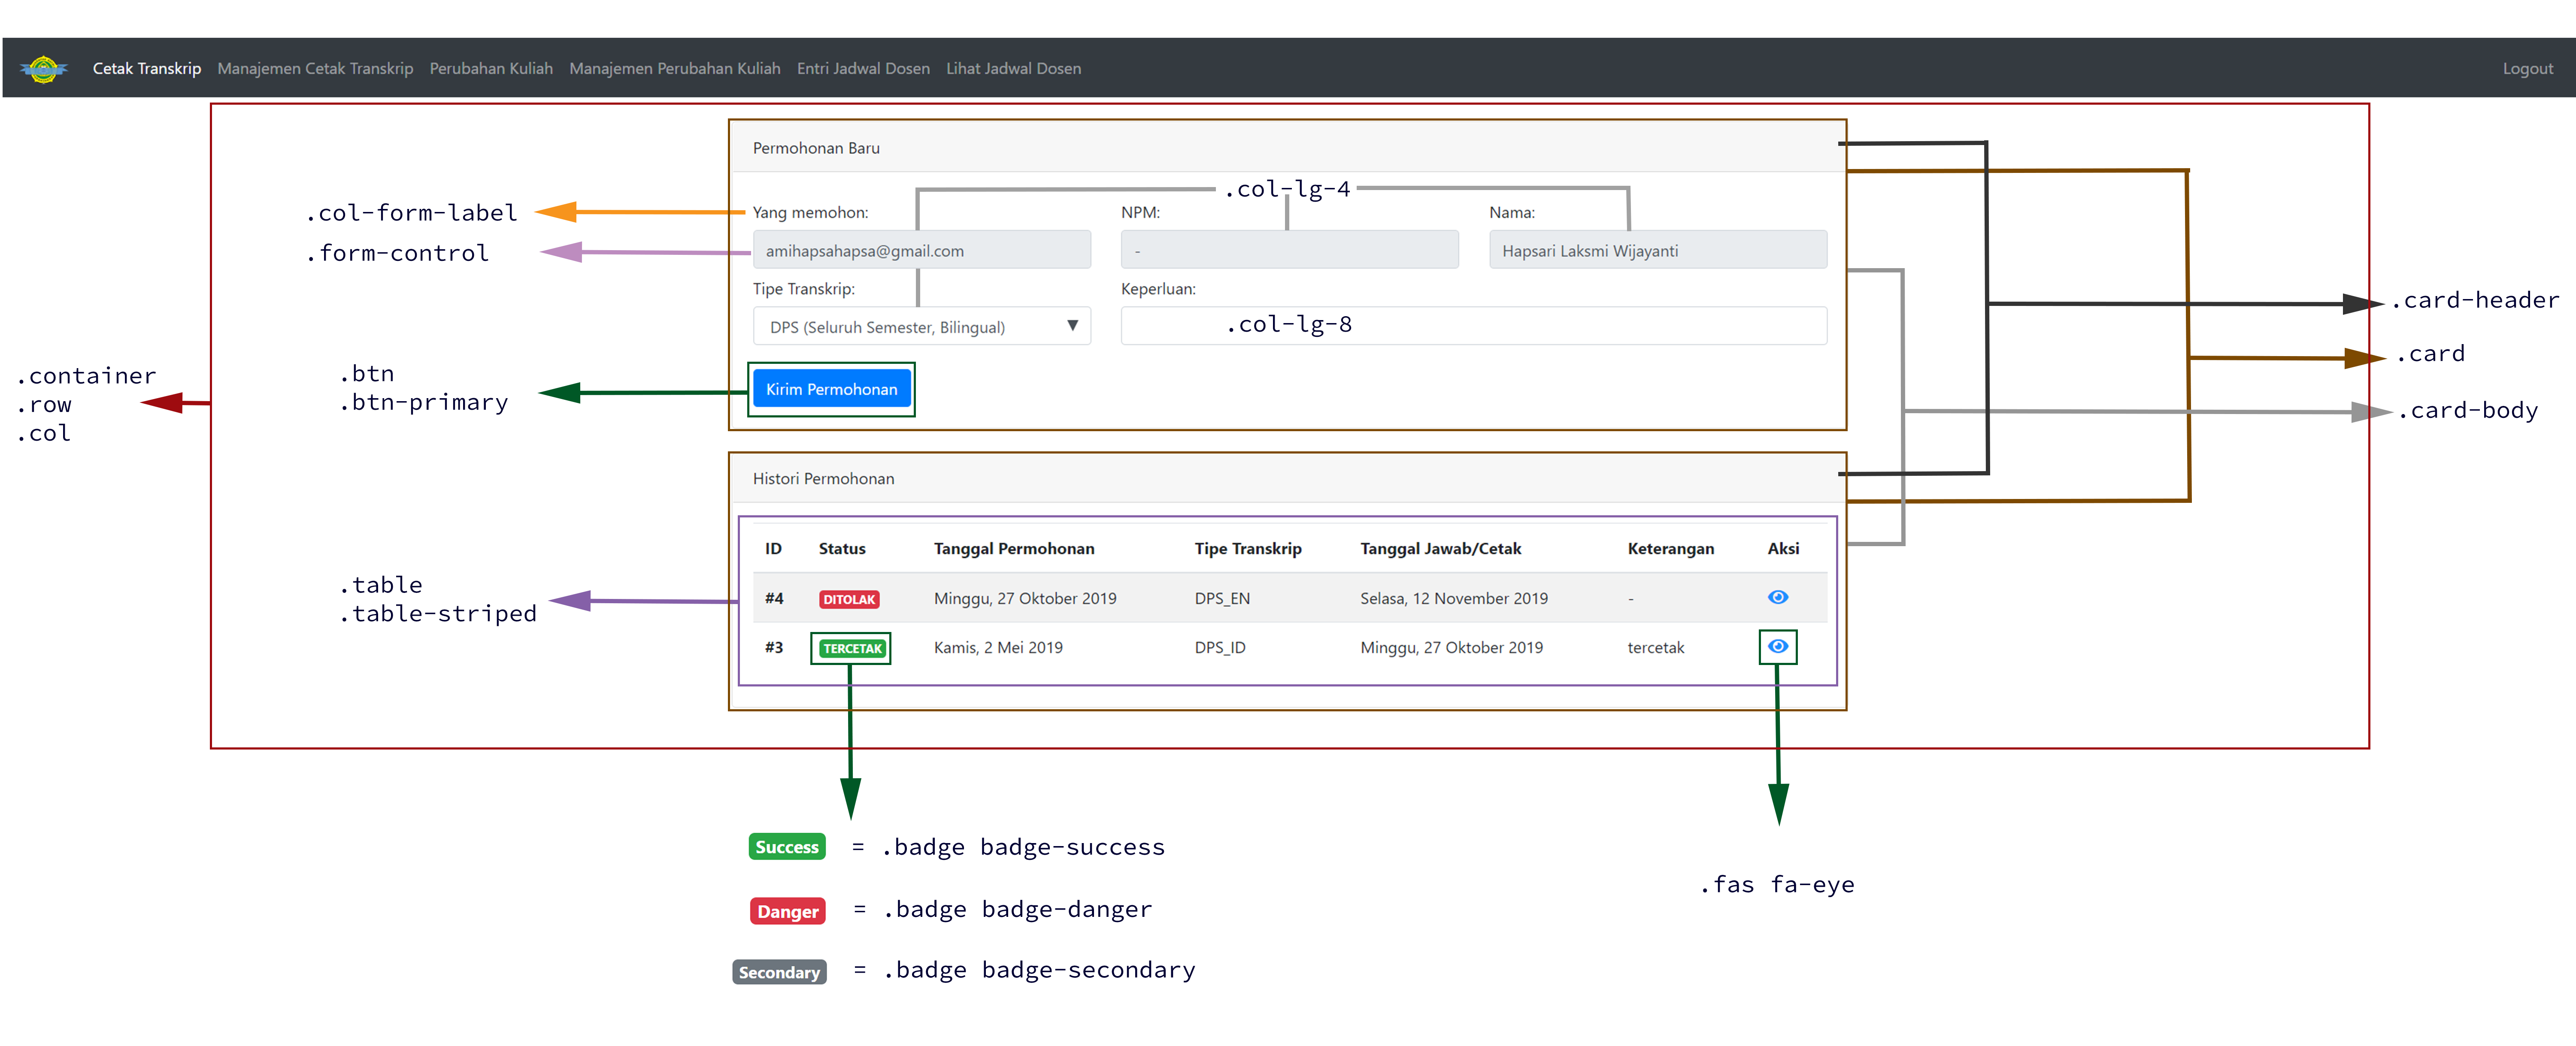
\includegraphics[width=\textwidth,height=\textheight,keepaspectratio]{bootstrap/konversi_tampilan_cetak_transkrip.png}
	\caption{Konversi halaman cetak transkrip.} 
	\label{fig:konversiPermintaanCetakTranskrip}
\end{figure}

Perubahan halaman permintaan cetak transkrip dilampirkan dalam Kode ~\ref{lst:mainTranskripRequest}.
\begin{lstlisting}[language=diff, caption=Perubahan file \path{\views\TranskripRequest\main.php} ,  basicstyle=\ttfamily, frame=single,
columns=fullflexible, keepspaces=true, breaklines=true, label={lst:mainTranskripRequest}]
diff -r a\www\application\views\TranskripRequest\main.php b\www\application\views\TranskripRequest\main.php
9c9,10
< 
---
> <br>
> <div class="container">

11,14c12,18
< <div class="medium-12 column">
< <div class="callout">
<     <h5>Permohonan Baru</h5>
<     <div class="callout alert">Transkrip akademik sementara dapat diakses via student portal masing-masing.</div>
---
> <div class="col">
>     <div class="card">
>         <div class="card-header">
>             Permohonan Baru
>         </div>
>         <div class="card-body">
> 

19,22c23,25
< <div class="large-4 column">
<     <label>Yang memohon:
<         <input type="email" name="requestByEmail" value="<?= $requestByEmail ?>" readonly="readonly"/>
<     </label>
---
> <div class="col-lg-4 form-group">
>     <label class="col-form-label">Yang memohon:</label>
>     <input class="form-control" type="email" name="requestByEmail" value="<?= $requestByEmail ?>" readonly/>

60,62c66,73
< <div class="callout">
<     <h5>Histori Permohonan</h5>
<     <table class="stack">
---
> </div>
> <br>
> <div class="card">
>  <div class="card-header">
>     Histori Permohonan
>  </div>
>  <div class="card-body table-responsive">
>     <table class="table table-striped">

65c76
< <th>ID</th>
---
> <th scope="col">ID</th>

77,78c88,89
< <td>#<?= $request->id ?></td>
< <td><span class="<?= $request->labelClass ?> label"><?= $request->status ?></span></td>
---
> <th>#<?= $request->id ?></th>
> <td><span class="badge badge-<?= $request->labelClass ?>"><?= $request->status ?></span></td>
\end{lstlisting}
Kode lengkap dari file ini dapat dilihat dalam lampiran ~\ref{lst:restranskripRequest}.

\noindent Catatan untuk kode ~\ref{lst:mainTranskripRequest} dijabarkan dalam tabel ~\ref{table:kodePermintaanCetakTranskrip}:
\begin{table}[H]
	\centering
	\caption{Penjelasan kode permintaan cetak transkrip.}
	\begin{tabularx}{\textwidth}{llX}
		\toprule
		No Line & Implementasi     & Penjelasan\\
		\midrule
		6 & \textbf{Container} & kelas \texttt{.container} dipakai pada Bootstrap untuk mengaktifkan sistem grid.\\
		10, 15 & \textbf{Konten} & Dalam Bootstrap 4 pembagian konten menggunakan \texttt{.card} yang terdiri dari \texttt{.card-header} dan \texttt{card-body} sedangkan di Foundation 6 hanya menggunakan kelas \texttt{.callout}. \\
		24, 29 & \textbf{Form Label} & Field pada Foundation 6 hanya menggunakan tag \texttt{<label>} sedangkan pada Bootstrap 4 menggunakan kelas \texttt{.col-form-label}.\\
		24, 29 & \textbf{Form input} & Field pada Foundation 6 hanya menggunakan tag \texttt{<input>} sedangkan pada Bootstrap 4 menggunakan kelas \texttt{.form-control}.\\
		47, 49 & \textbf{Thread} & Pada Foundation 6 hanya menggunakan tag html \texttt{<th>} sedangkan pada Bootstrap 4 menggunakan memerlukan \texttt{scope="col"}.\\
		53, 56 & \textbf{Label} & Pada Foundation 6 menggunakan komponen label dengan memanfaatkan kelas \texttt{label}, sedangkan di Bootstrap 4 menggunakan komponen \textit{badges} dengan memanfaatkan kelas \texttt{.badge}.\\
		
		\bottomrule
	\end{tabularx}%
	\label{table:kodePermintaanCetakTranskrip}
\end{table}

\subsection{Halaman Manajemen Cetak Transkrip} 
Halaman ini terdiri dari satu konten yaitu "Permintaan Transkrip" tertera pada gambar ~\ref{fig:analisisManajemenCetakTranskrip}. Bagian form pencarian NPM menggunakan \textit{group field}, dimana nama form , isi form dan tombol merupakan satu kesatuan. Lalu dibawah form terdapat tabel yang menampilkan data permintaan cetak transkrip. 
\begin{figure} [H]
	\centering  
	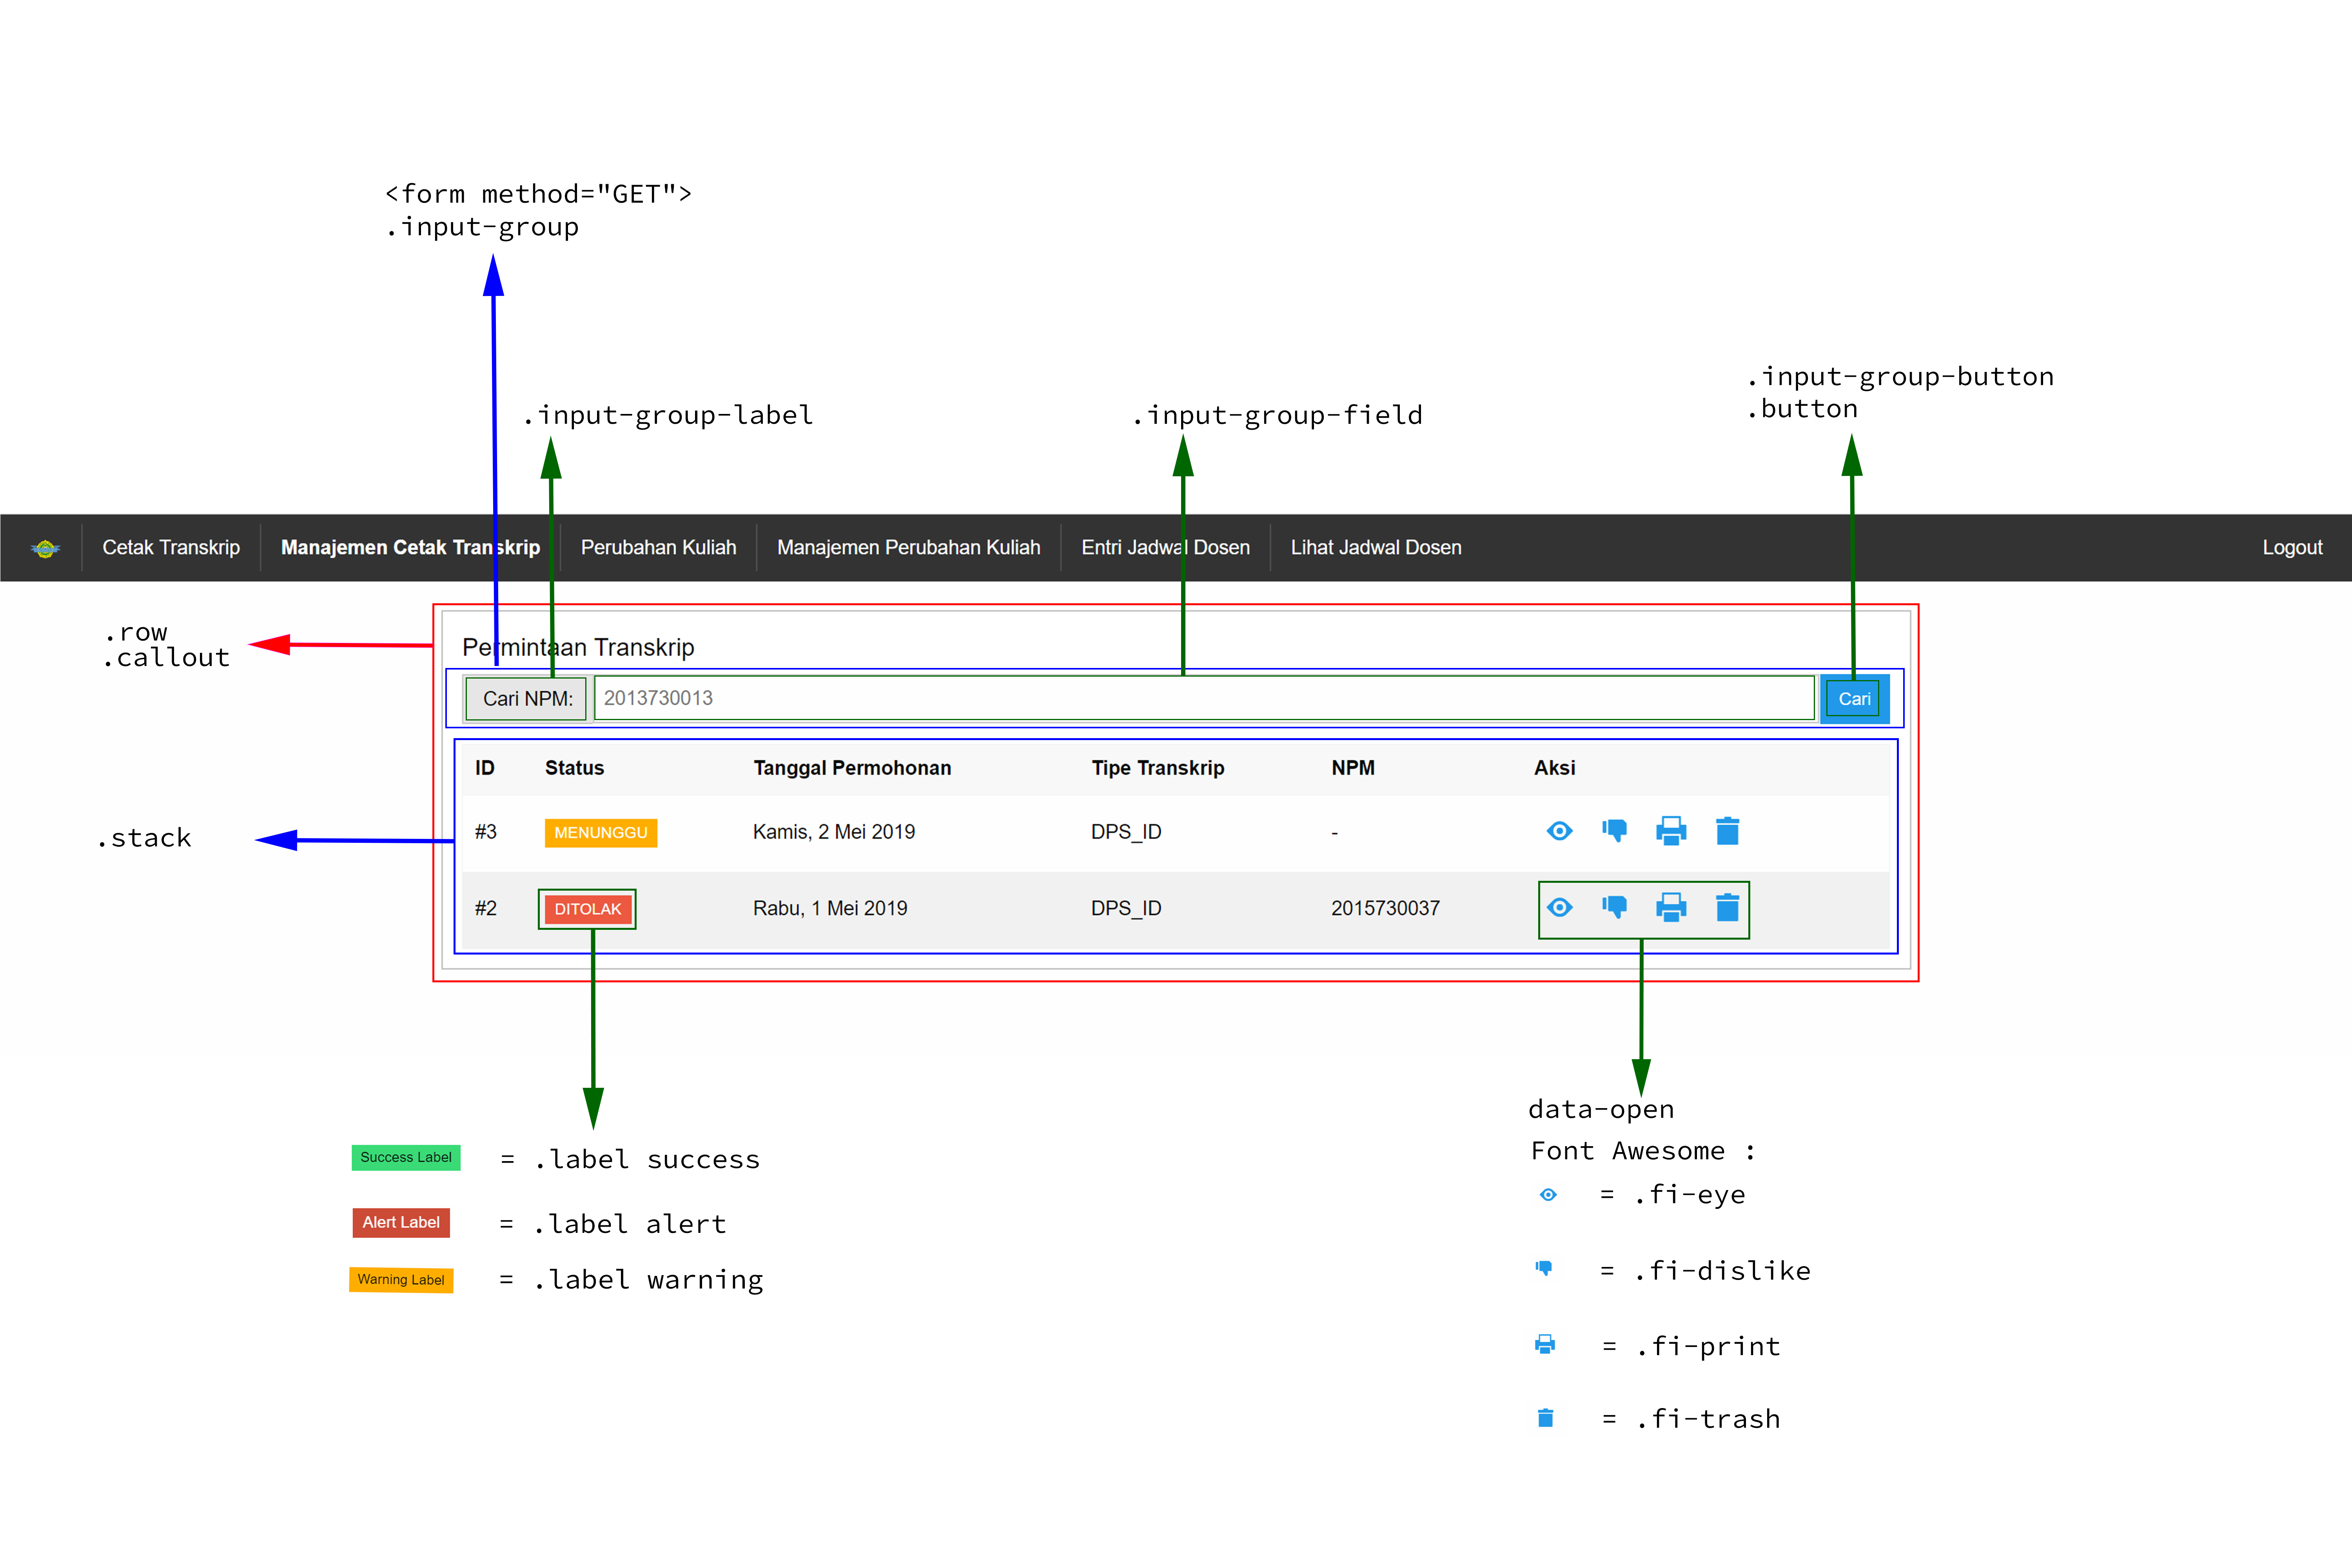
\includegraphics[width=\textwidth,height=\textheight,keepaspectratio]{foundation/analisis_manajemen_cetak_transkrip.png}
	\caption{Analisis manajemen cetak transkrip.} 
	\label{fig:analisisManajemenCetakTranskrip}
\end{figure} 

\noindent Gambar ~\ref{fig:konversiManajemenCetakTranskrip} menjelaskan komponen dalam website beserta penamaan kelas untuk Bootstrap 4 pada halaman manajemen cetak transkrip.\\
\begin{figure} [H]
	\centering  
	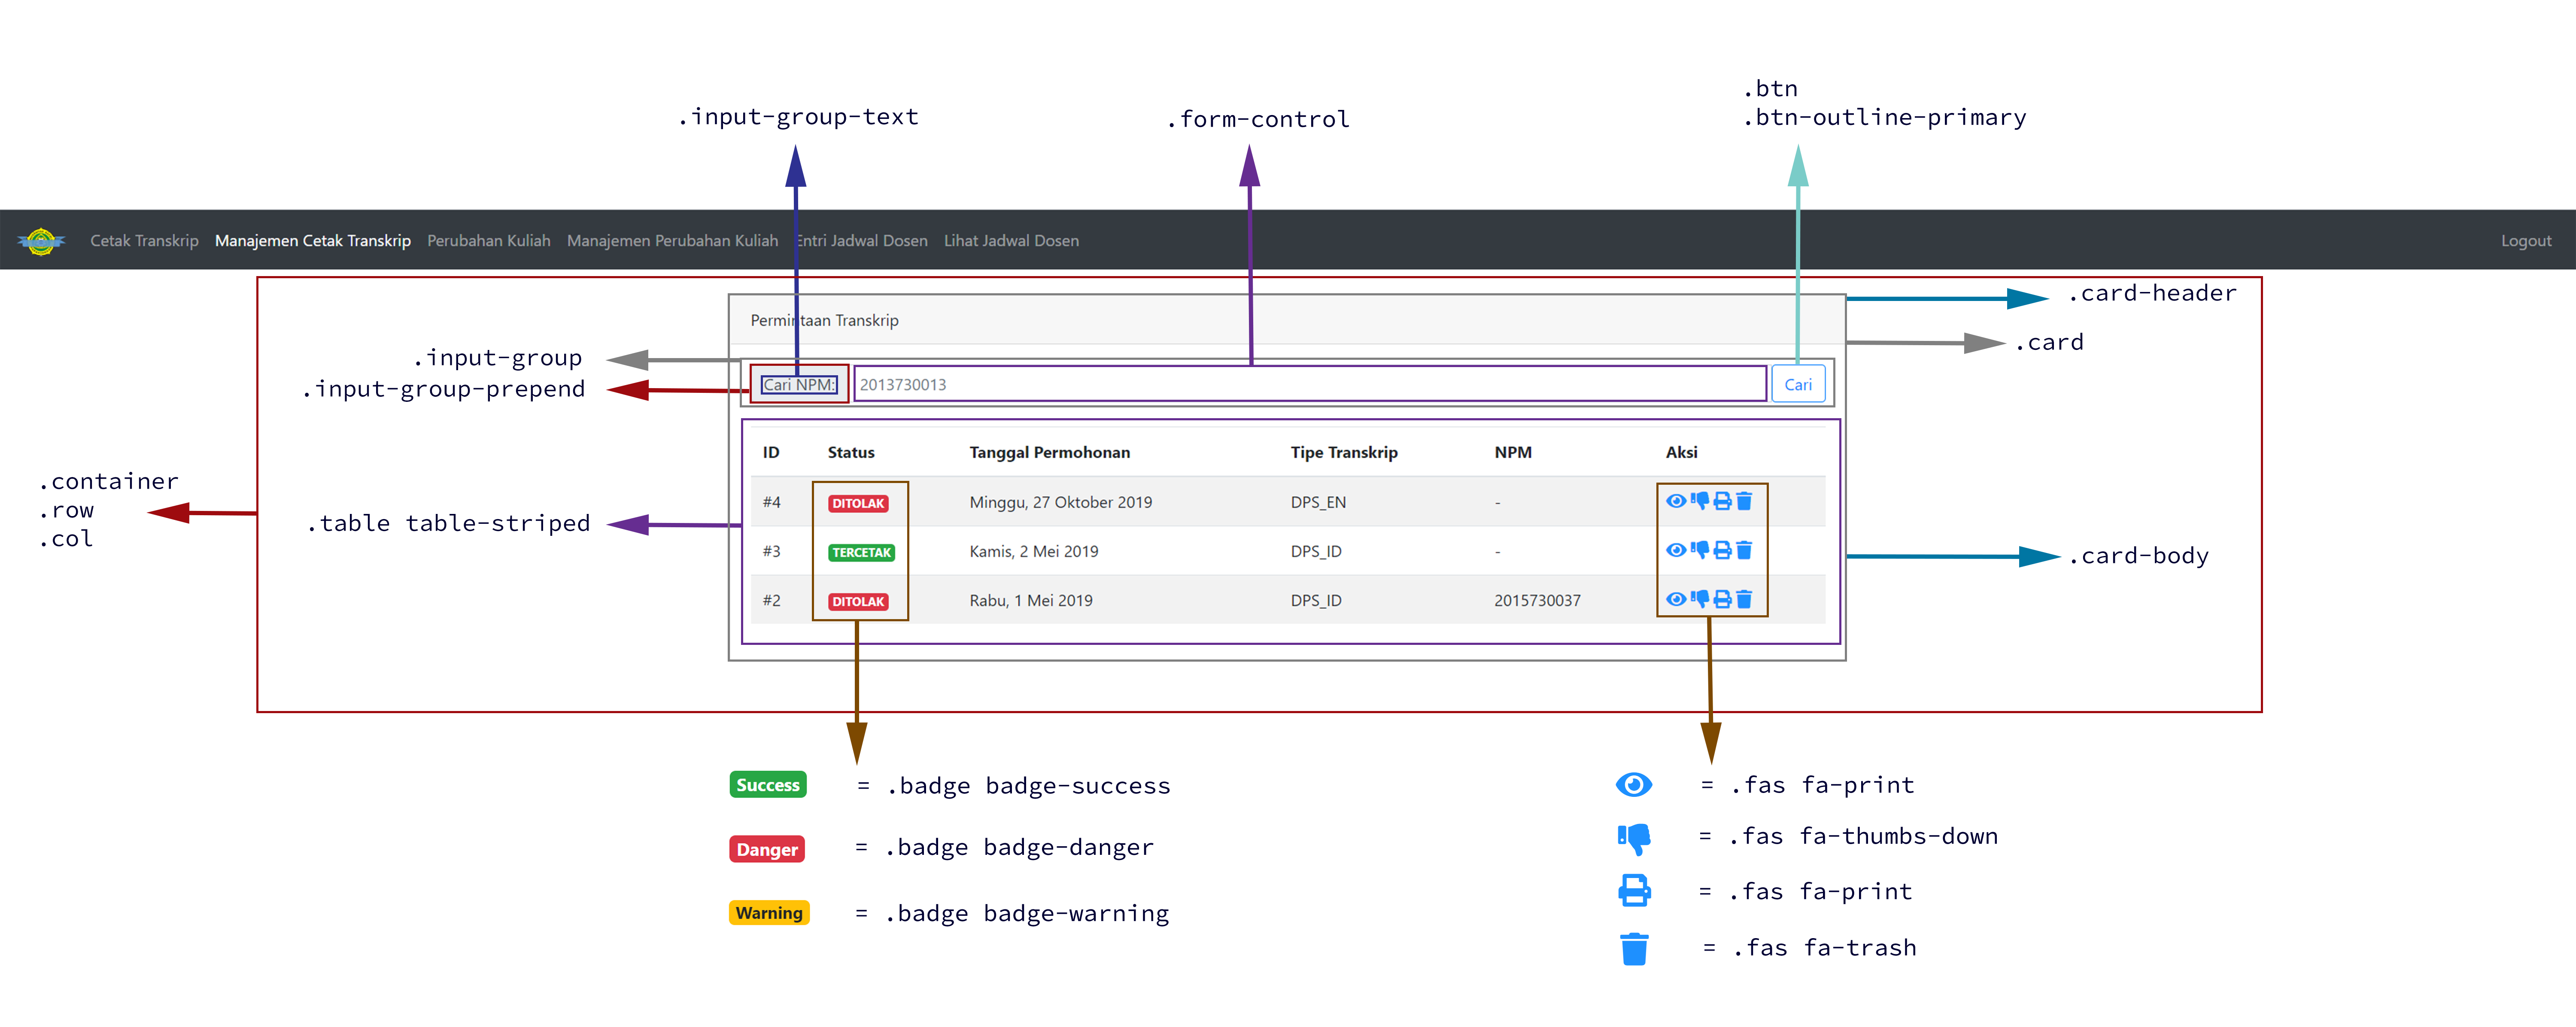
\includegraphics[width=\textwidth,height=\textheight,keepaspectratio]{bootstrap/konversi_tampilan_manajemen_cetak_transkrip.png}
	\caption{Konversi manajemen cetak transkrip.} 
	\label{fig:konversiManajemenCetakTranskrip}
\end{figure}

Pada kode ~\ref{lst:mainTranskripManage} menjelaskan perubahan kode pada halaman manajemen permintaan transkrip.

\begin{lstlisting}[language=diff, caption=Perubahan file \path{\views\TranskripManage\main.php},  basicstyle=\ttfamily, frame=single,
columns=fullflexible, keepspaces=true, breaklines=true, label={lst:mainTranskripManage}]
diff -r a\www\application\views\TranskripManage\main.php b\www\application\views\TranskripManage\main.php

15c18,20
< 	<span class="input-group-label">Cari NPM:</span>
---
> <div class="input-group-prepend">
>     <span class="input-group-text">Cari NPM:</span>
> </div>

16,18c22,24
< <input name="npm" class="input-group-field" type="text" placeholder="2013730013" maxlength="10" minlength="10"<?= $npmQuery === NULL ? '' : " value='$npmQuery'" ?>/>
< <div class="input-group-button">
<     <input class="button" type="submit" value="Cari"/>
---
> <input name="npm" class="form-control" type="text" placeholder="2013730013" maxlength="10" minlength="10"<?= $npmQuery === NULL ? '' : " value='$npmQuery'" ?>/>
> <div class="input-group-append">
>     <input class="btn btn-primary" type="submit" value="Cari"/>

22c29
<  <table class="stack">
---
> <table class="table table-striped">


87c87,88
> <a data-toggle="modal" data-target="#detail<?= $request->id ?>" id="detailIkon<?= $request->id ?>">
>     <i class="fas fa-eye"></i>
> </a>

88c88
<     <a data-open="detail<?= $request->id ?>"><i class="fi-eye"></i></a>


102c131,133
<     <input type="submit" class="alert button" value="Tolak"/>
---
>     <div class="form-group">
>         <input type="submit" class="btn btn-danger" value="Tolak"/>
>     </div>

\end{lstlisting}
Kode lengkap dari file ini dapat dilihat dalam lampiran ~\ref{lst:restranskripManage}.

\noindent Catatan untuk kode ~\ref{lst:mainTranskripManage} dijabarkan dalam tabel ~\ref{tabel:KodeManajemenCetakTranskrip}:
\begin{table}[H]
	\centering
	\caption{Penjelasan kode konversi manajemen cetak transkrip.}
	\begin{tabularx}{\textwidth}{llX}
		\toprule
		No & Implementasi     & Penjelasan \\
		\midrule
		4, 7 & \textbf{Input group label} & Foundation 6 menggunakan kelas \texttt{input-group-label} sedangkan Bootstrap 4 menggunakan  \texttt{input-group-text} untuk menandakaan elemen tersebut adalah label dari input group.\\
		11, 15 & \textbf{Input group field} & Foundation 6 menggunakan kelas \texttt{input-group-label} sedangkan Bootstrap 4 menggunakan  \texttt{.form-control} untuk menandakaan elemen tersebut adalah field dari input group.\\
		13, 17 & \textbf{Input group button} & Foundation 6 menggunakan kelas \texttt{input-group-button} sedangkan Bootstrap 4 menggunakan  \texttt{.btn} untuk menandakaan elemen tersebut adalah button dari input group.\\
		6 & \textbf{Prepend} & Pada Bootstrap 4 harus didefinisikan letak elemen, dengan  menggunakan  \texttt{input-group-prepend} maka elemen terletak didepan input.\\
		16 & \textbf{Append} & Pada Bootstrap 4 harus didefinisikan letak elemen, dengan  menggunakan  \texttt{input-group-prepend} maka elemen terletak dibelakang input.\\
		\bottomrule
	\end{tabularx}%
	\label{tabel:KodeManajemenCetakTranskrip}
\end{table}

\subsection{Halaman Permintaan Perubahan Kuliah}
Halaman permintaan perubahan kuliah terdiri dari dua konten: "Permohonan Baru" dan "Histori Permohonan" tertera pada gambar ~\ref{fig:analisisPermintaanPerubahanKuliah}. 

Setiap konten dipisahkan oleh border dalam Foundation disebut \texttt{callout}. Pada "Permohonan Baru" terdapat sebuah form yang berisi field-fiel dengan lebar yang berbeda - beda dan dikelompokan pada beberapa baris. Terdapat tiga tombol yaitu tombol biru "Kirim Permohonan" dan tombol abu-abu "Tambah pertemuan Ektra" .
Konten "Histori Permohonan" berisi tabel bergaris yang menampilkan data histori permohonan. 
\begin{figure} [H]
	\centering  
	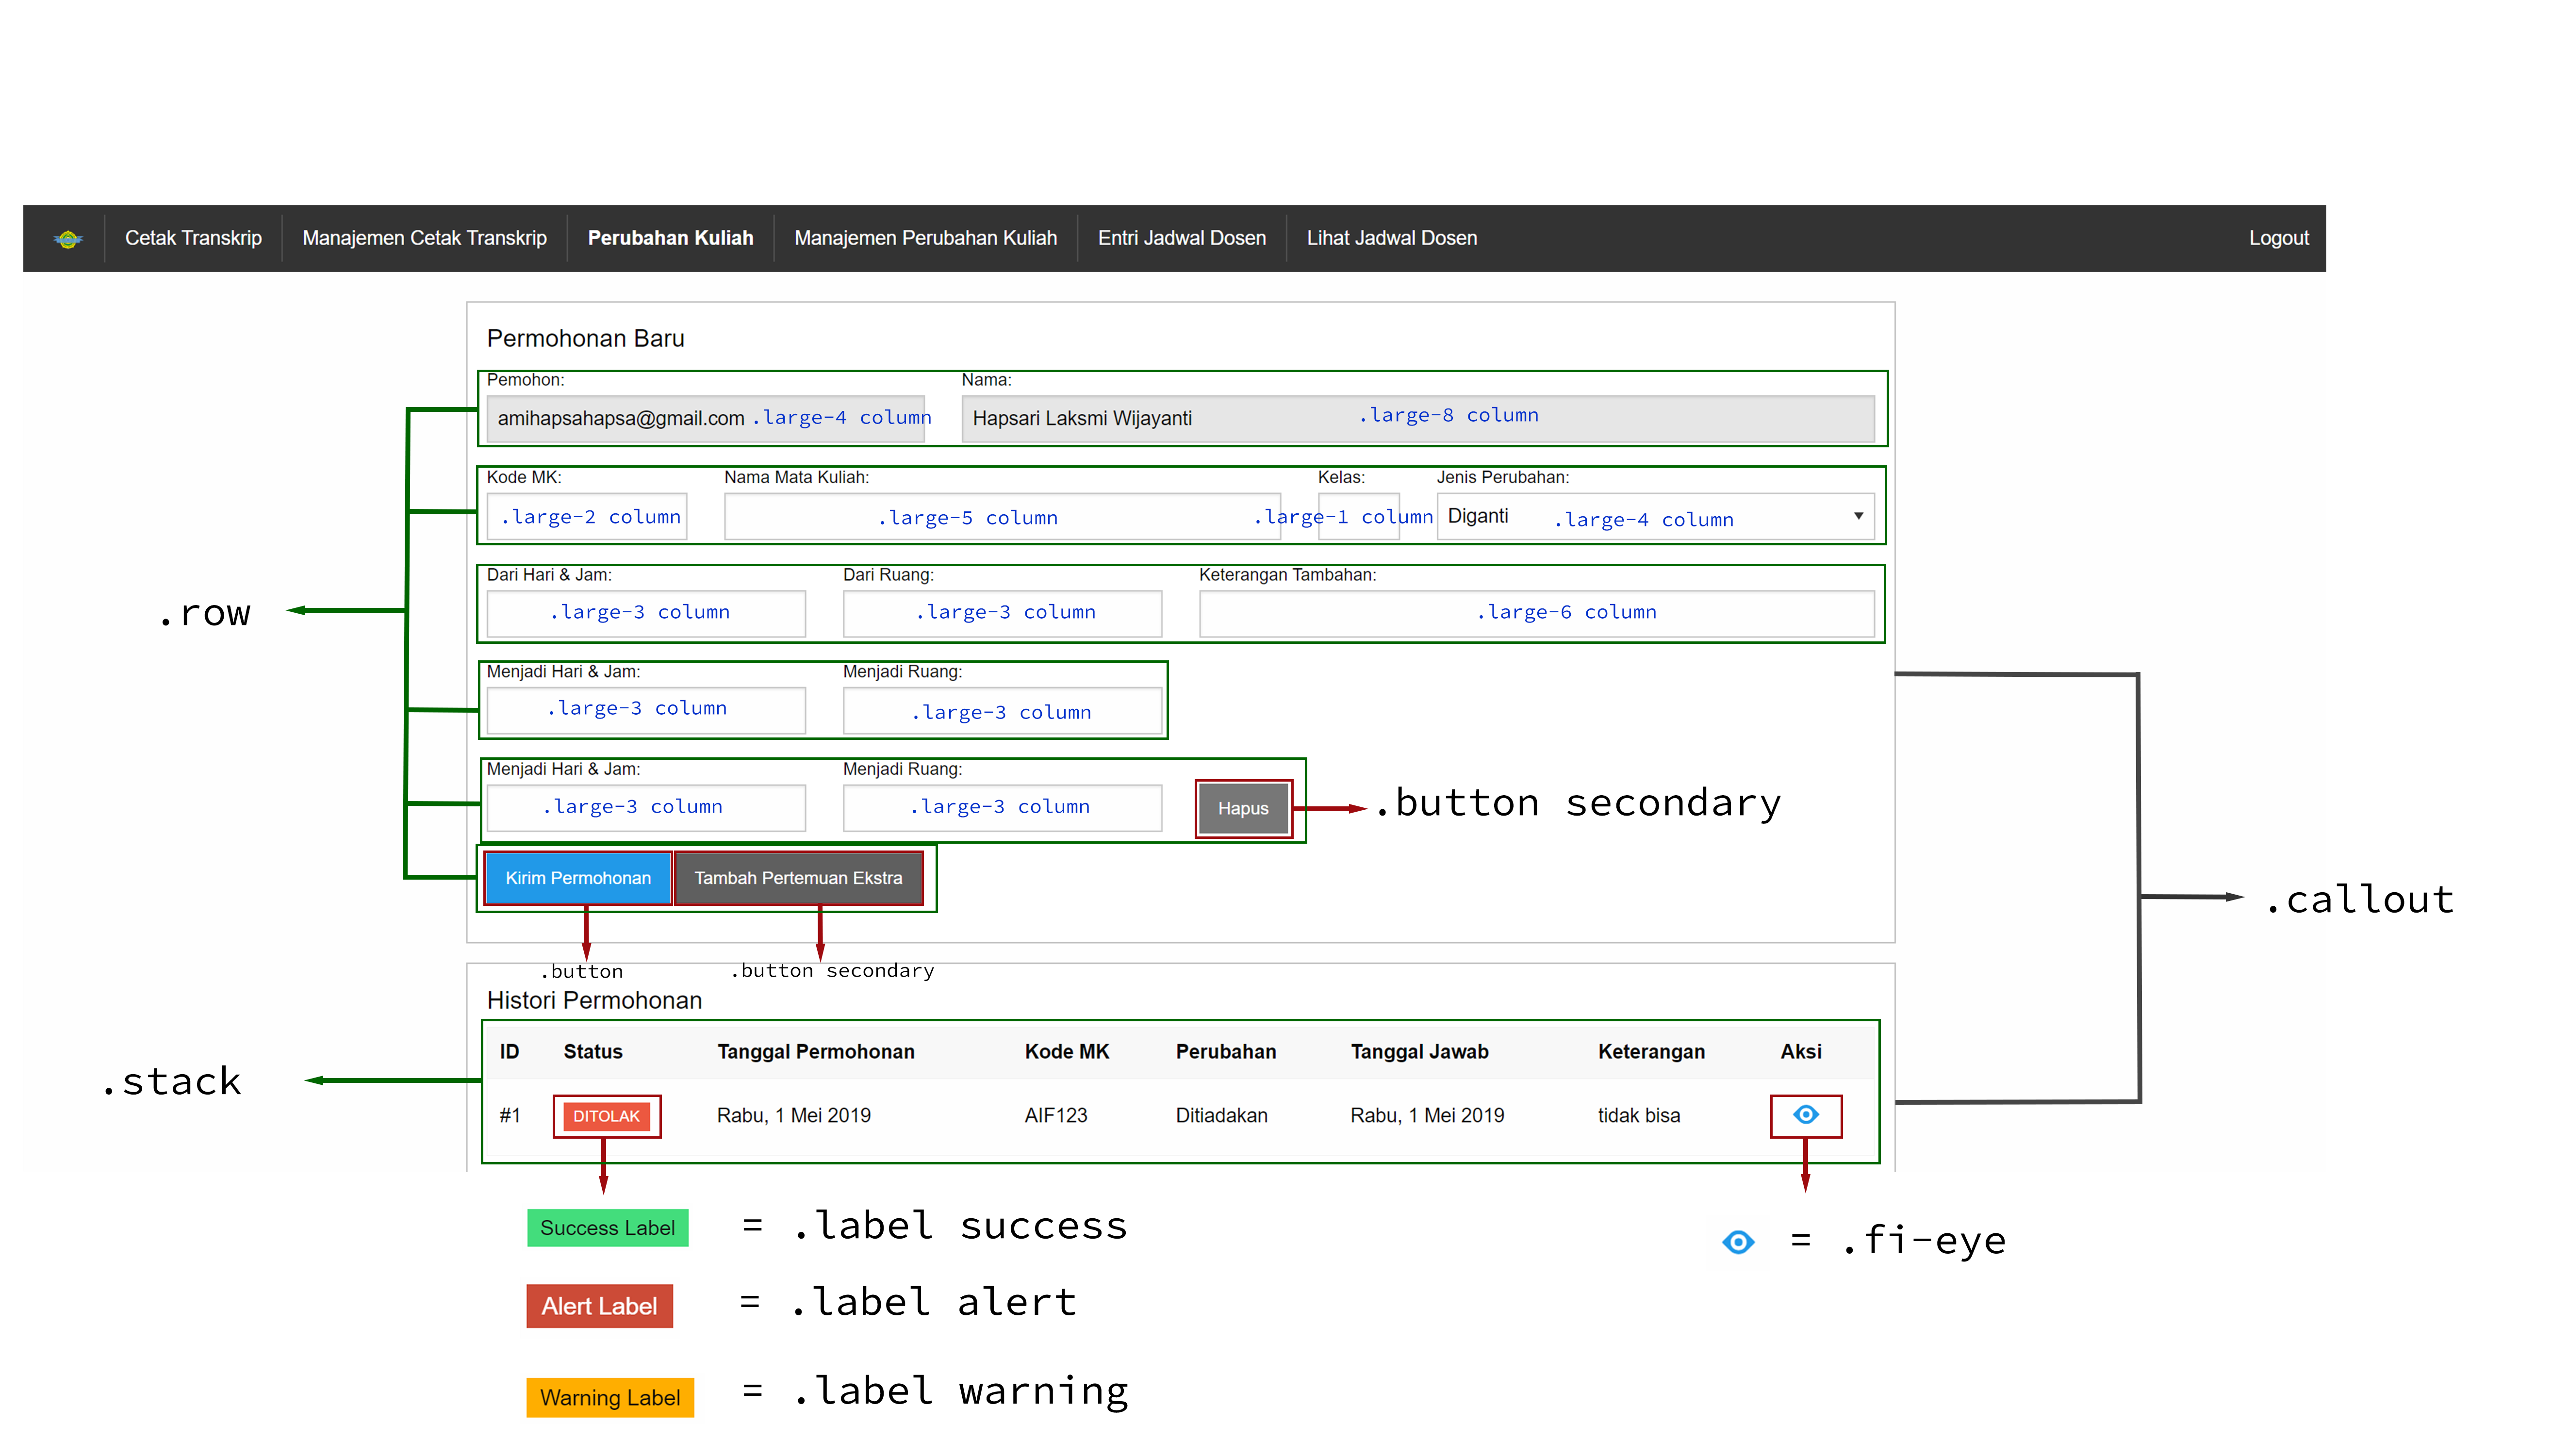
\includegraphics[width=\textwidth,height=\textheight,keepaspectratio]{foundation/analisis_perubahan_kuliah_request.png}
	\caption{Analisis halaman permintaan perubahan kuliah.}
	\label{fig:analisisPermintaanPerubahanKuliah}
\end{figure}

\noindent Gambar ~\ref{fig:konversiPermintaanPerubahanKuliah} menjelaskan komponen dalam website beserta penamaan kelas untuk Bootstrap 4 pada halaman permintaan perubahan kuliah.\\
\begin{figure} [H]
	\centering  
	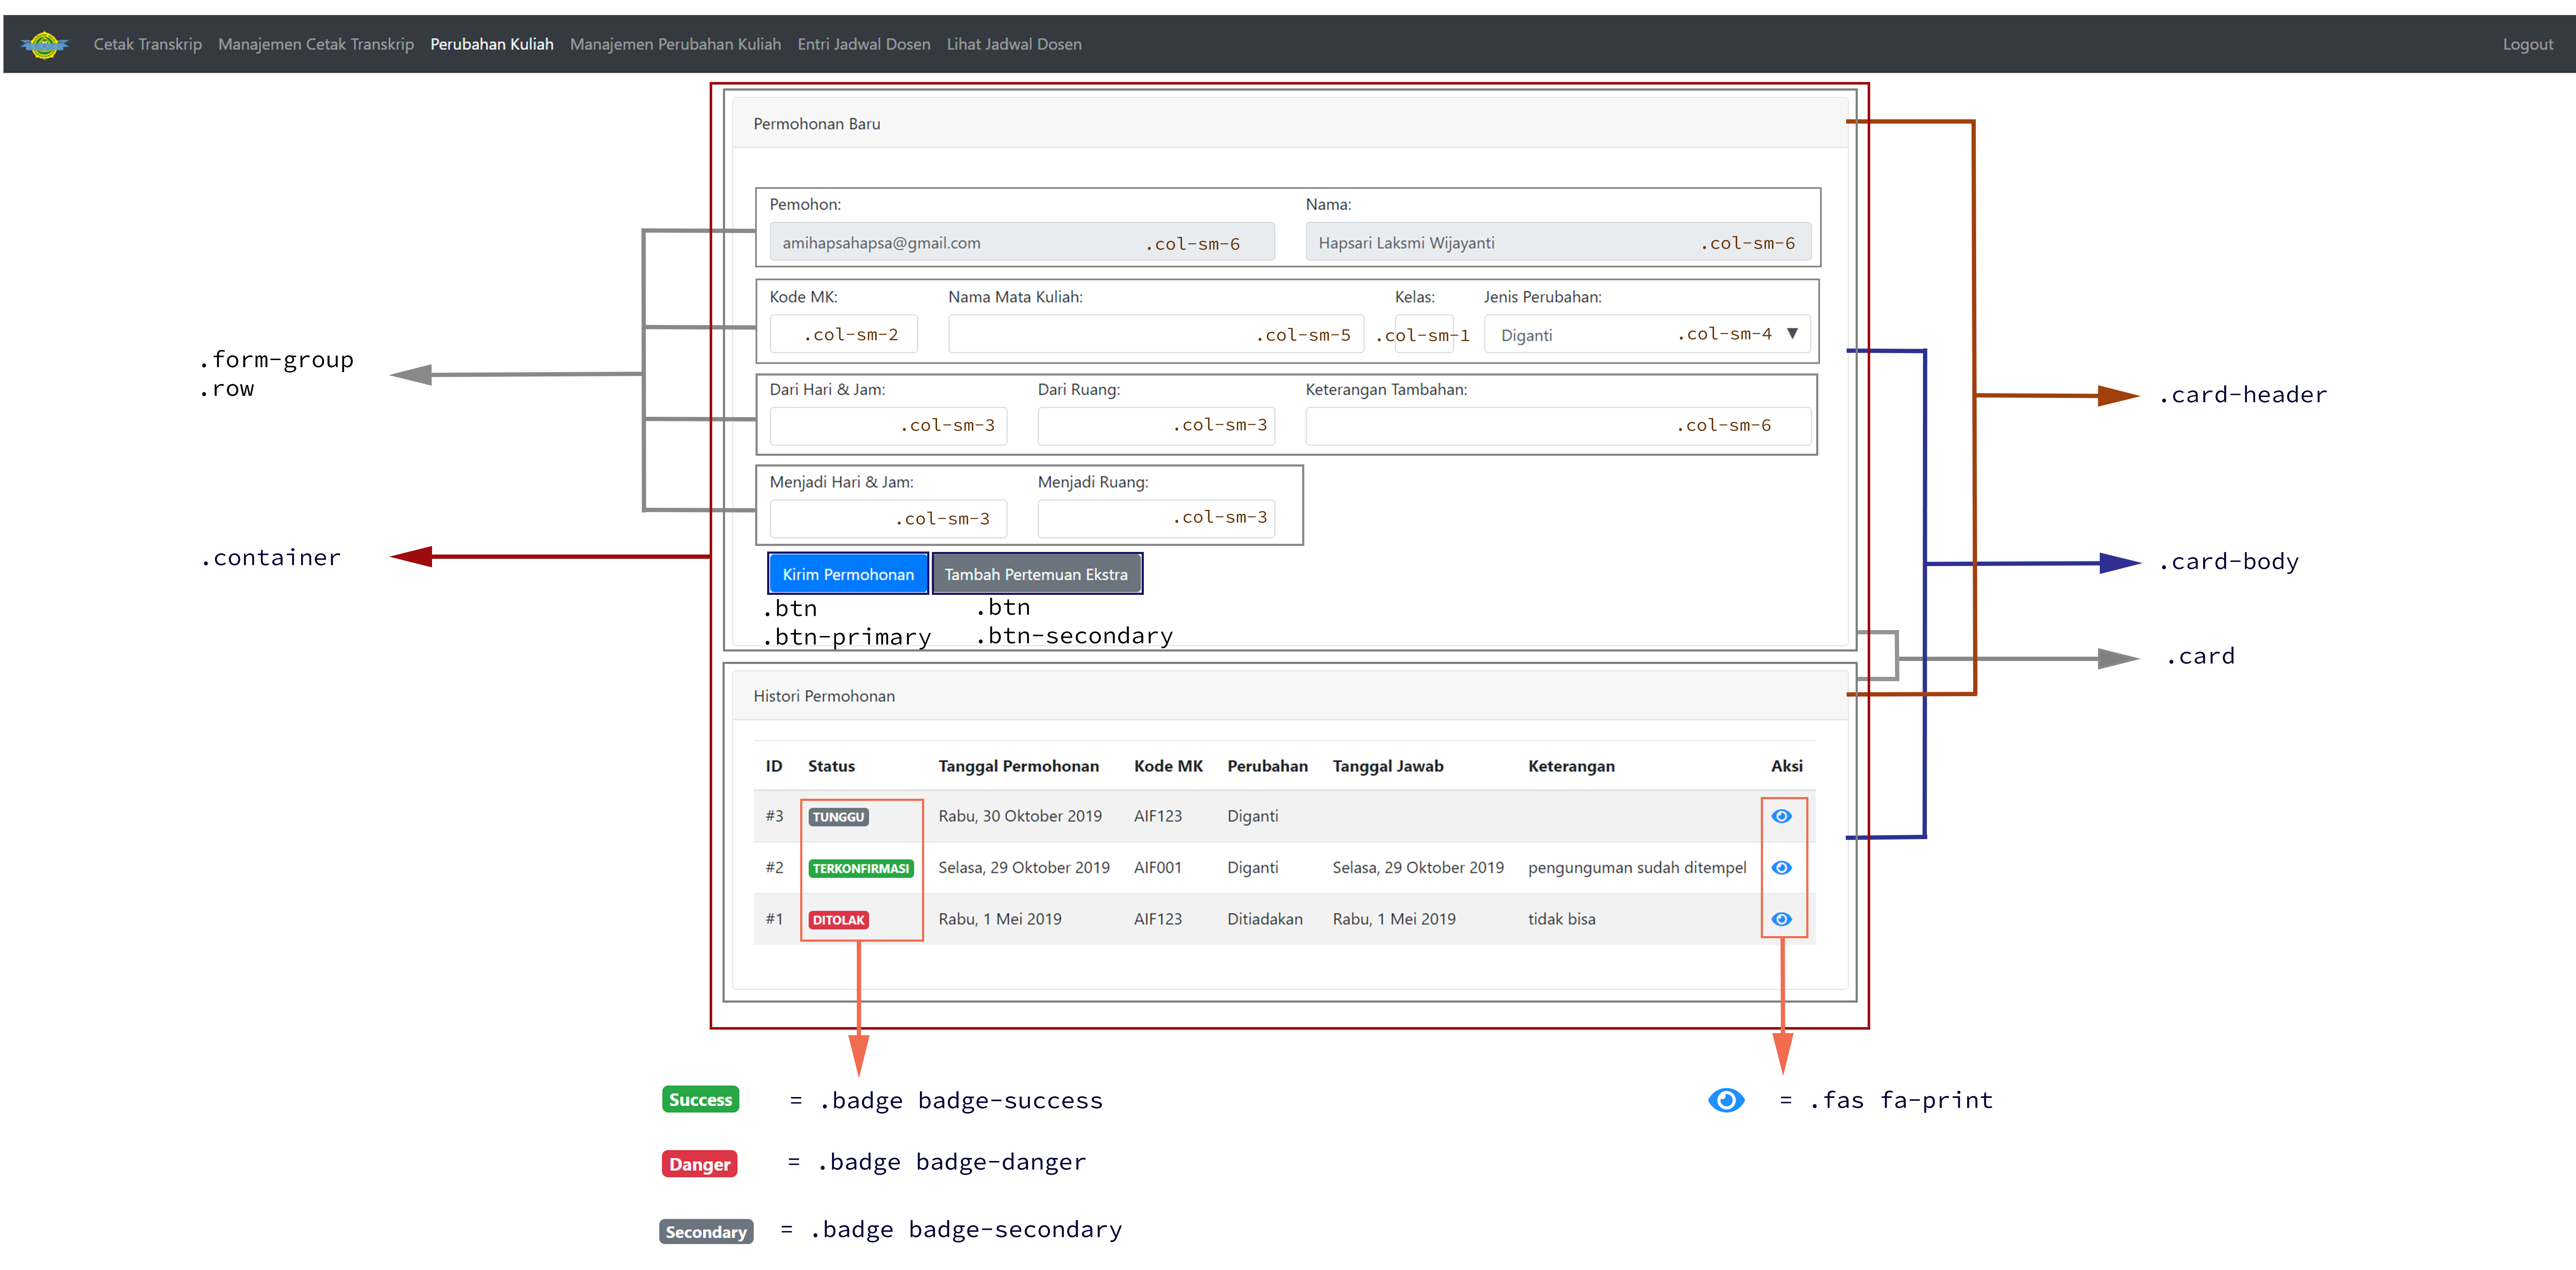
\includegraphics[width=\textwidth,height=\textheight,keepaspectratio]{bootstrap/konversi_tampilan_perubahan_kuliah.png}
	\caption{Konversi halaman permintaan perubahan kuliah.}
	\label{fig:konversiPermintaanPerubahanKuliah}
\end{figure}
\noindent Catatan untuk kode ~\ref{lst:mainPerubahanKuliahRequest} dijabarkan dalam tabel ~\ref{tabel:permintaanPerubahanKuliah}:

\begin{lstlisting}[language=diff, caption=Perubahan file \path{\views\PerubahanKuliahRequest\main.php} ,  basicstyle=\ttfamily, frame=single,
columns=fullflexible, keepspaces=true, breaklines=true, label={lst:mainPerubahanKuliahRequest}]
diff -r a\www\application\views\PerubahanKuliahRequest\main.php b\www\application\views\PerubahanKuliahRequest\main.php

96,98c88,95
< <div class="callout">
<     <h5>Histori Permohonan</h5>
<     <table class="stack">
---
> </div>
> <br>
> <div class="card">
>  <div class="card-header">
>     Histori Permohonan
>  </div>
>  <div class="card-body table-responsive">
>     <table class="table table-striped">
214a224
> jQuery('#datetimepicker').datetimepicker();
\end{lstlisting}
Kode lengkap dari file ini dapat dilihat dalam lampiran ~\ref{lst:resperubahanKuliahRequest}.

\begin{table}[H]
	\centering
	\caption{Penjelasan kode permintaan perubahan kuliah.}
	\begin{tabularx}{\textwidth}{llX}
		\toprule
		No & Implementasi     & Penjelasan \\
		\midrule	
		6, 14 &\textbf{Tabel} & Pada foundation 6 tabel menggunakan kelas \texttt{.stack} yang memungkinkan data tersusun secara vertikal. Pada bootstrap 4 fungsi tersebut tidak ada sehingga menggunakan alternatif kelas \texttt{table-responsive} yang memungkinkan tabel dapat bergerak secara horizontal pada \textit{device} atau \textit{tab}. \\
		17 &\textbf{Plugin} & Pada Bootstrap 4 perlu ditambahkan kode jQuery untuk menjalankan plugin \texttt{datetimepicker}. \\
		\bottomrule
	\end{tabularx}%
	\label{tabel:permintaanPerubahanKuliah}
\end{table}

\subsection{Halaman Manajemen Perubahan Kuliah}
Halaman pada gambar ~\ref{fig:analisisManajemenPerubahanKuliah} menampilkan data permohonan perubahan kuliah berisi sebuah tabel dimana pada kolom 'Status' menggunakan kelas \texttt{.callout} untuk \textit{highlight} status dan pada kolom 'Aksi' menampilkan lima jenis ikon dari \textit{Library} Font Awesome. Setiap ikon merupakan link menuju modal.
\begin{figure} [H]
	\centering  
	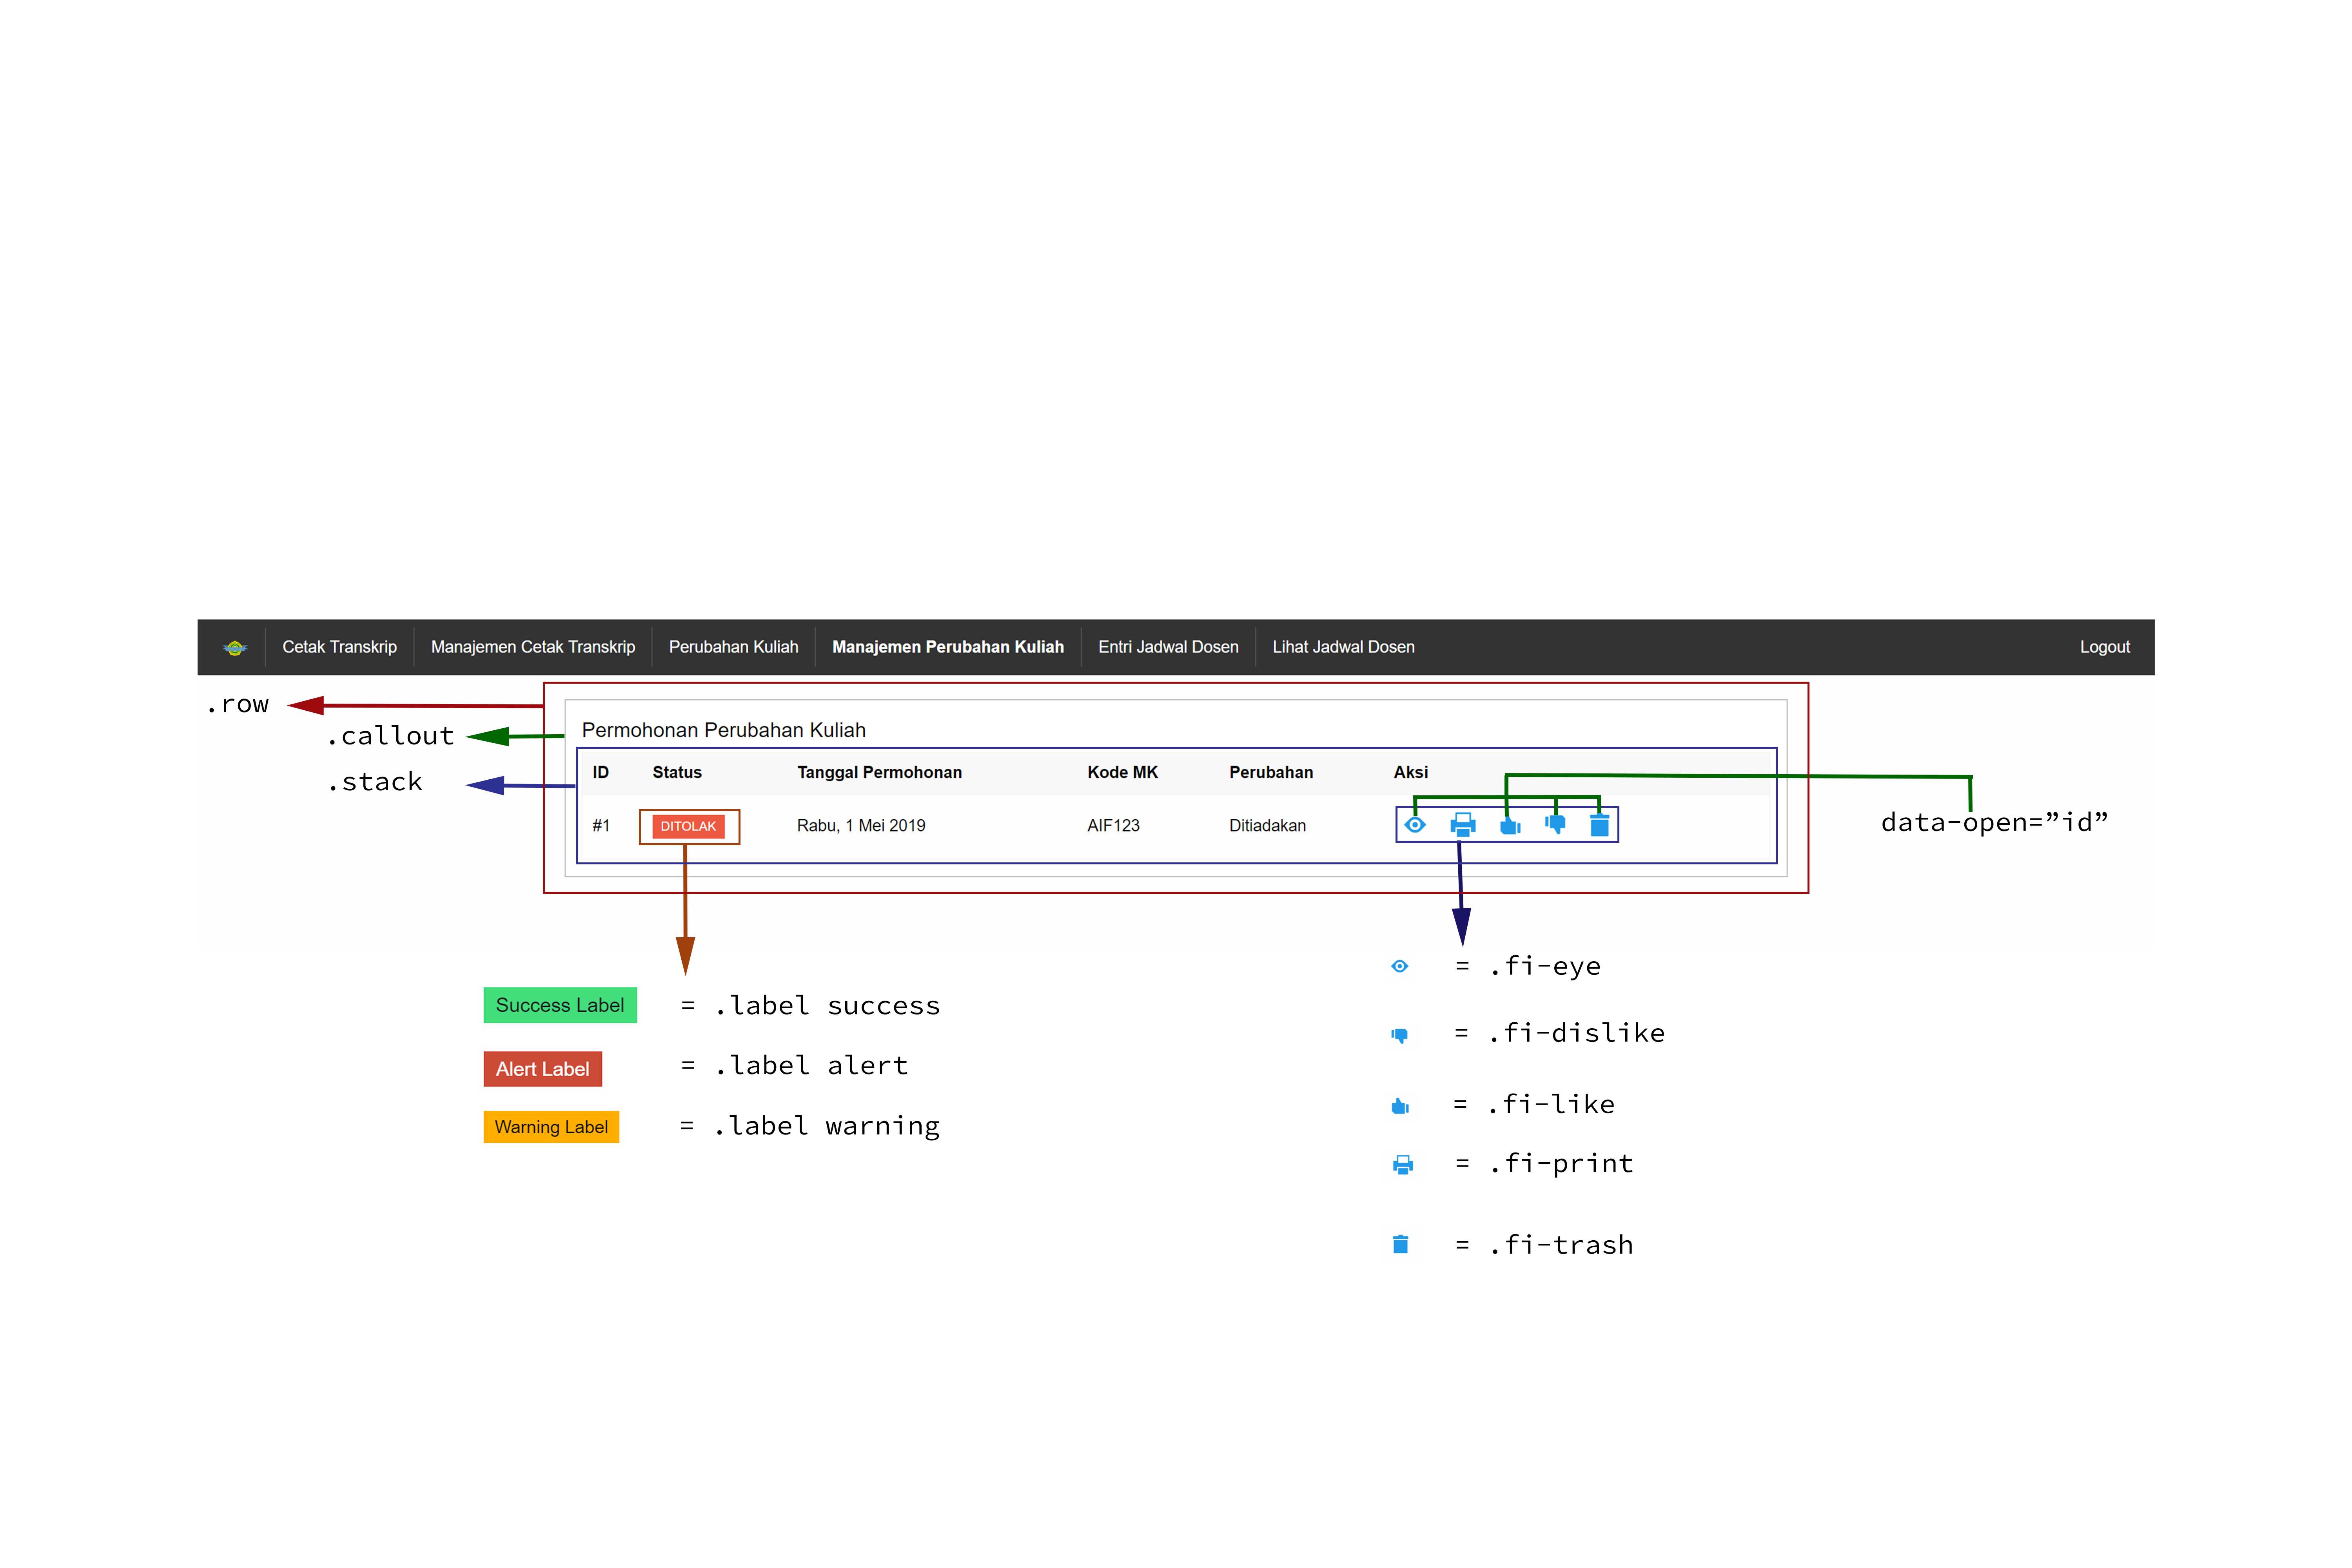
\includegraphics[width=\textwidth,height=\textheight,keepaspectratio]{foundation/analisis_manajemen_perubahan_kuliah.png}
	\caption{Analisis halaman manajemen perubahan kuliah.}
	\label{fig:analisisManajemenPerubahanKuliah}
\end{figure}
\noindent Gambar ~\ref{fig:konversiManajemenPerubahanKuliah} menjelaskan komponen dalam website beserta penamaan kelas untuk Bootstrap 4 pada halaman manajemen perubahan kuliah.\\
\begin{figure} [H]
	\centering  
	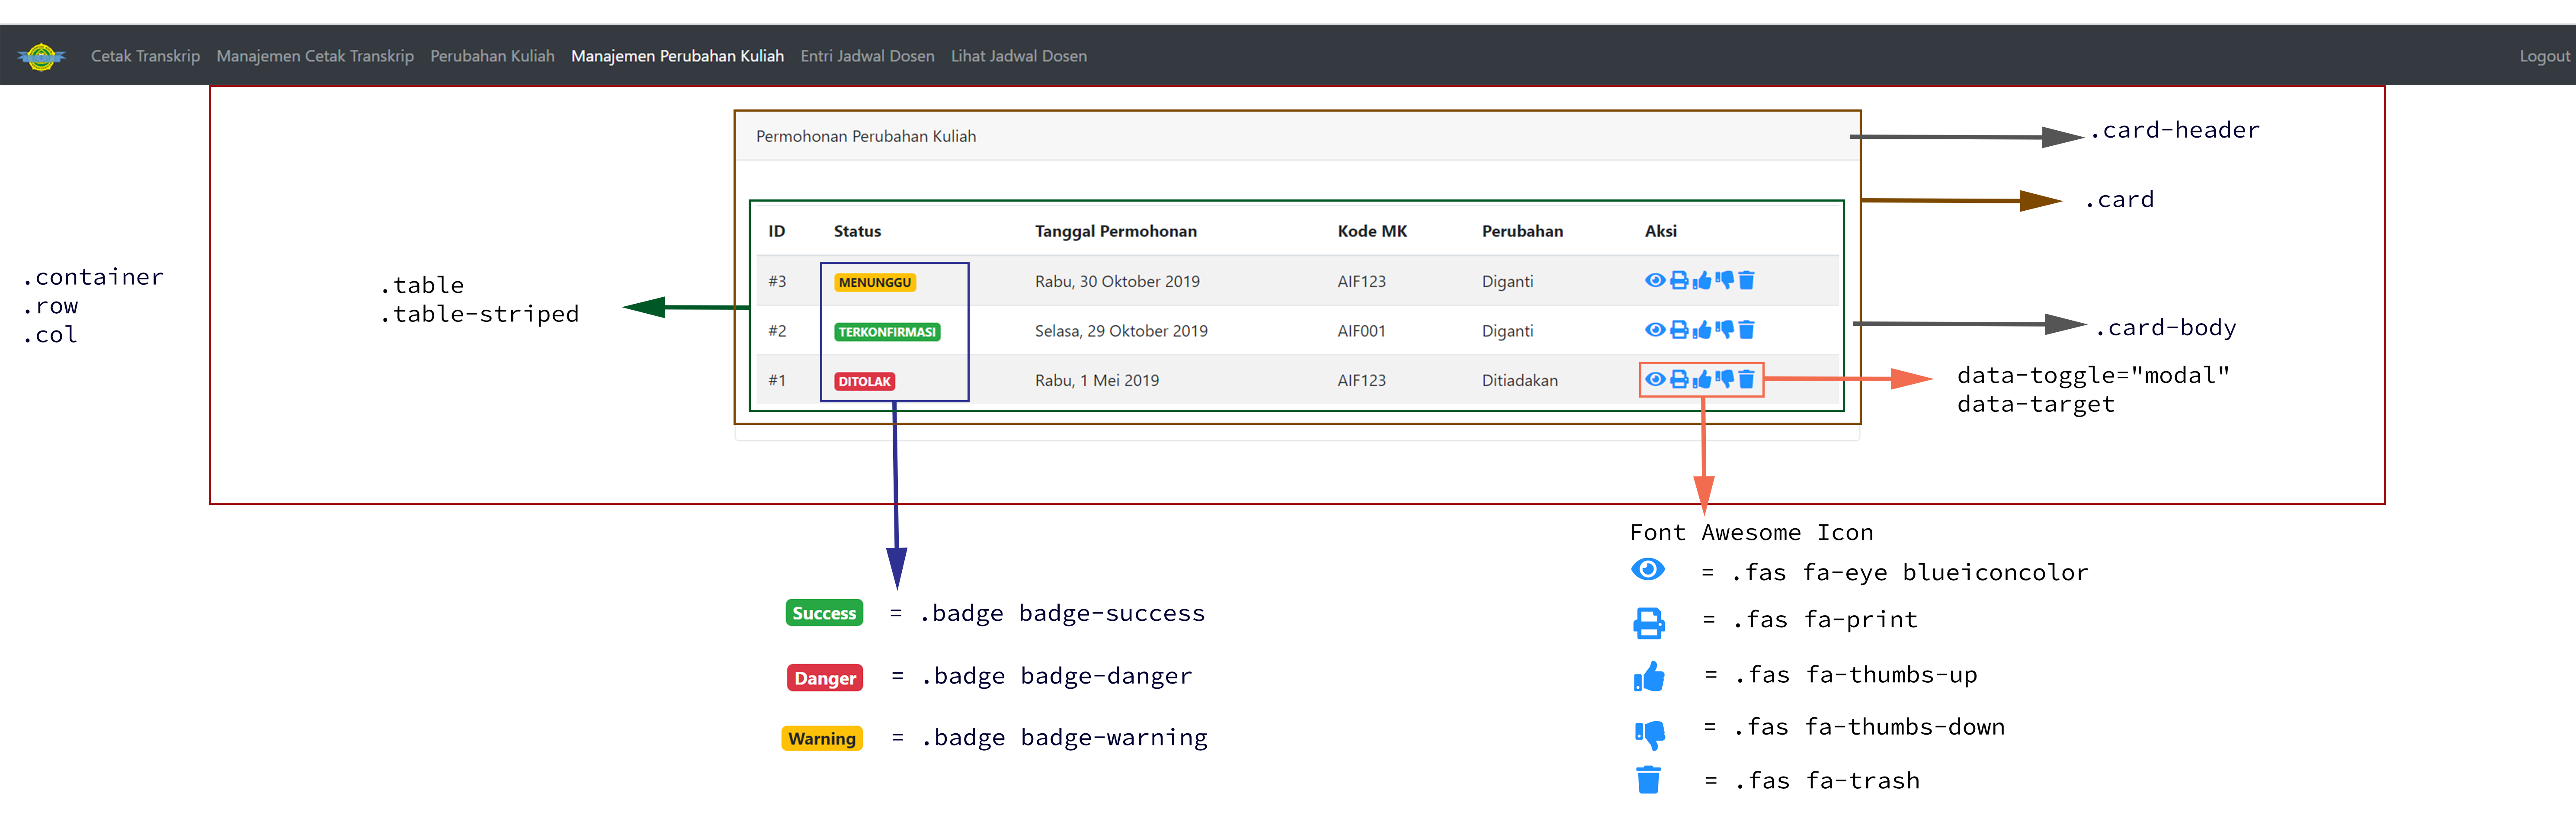
\includegraphics[width=\textwidth,height=\textheight,keepaspectratio]{bootstrap/konversi_tampilan_manajemen_perubahan_kuliah.png}
	\caption{Konversi halaman manajemen perubahan kuliah.}
	\label{fig:konversiManajemenPerubahanKuliah}
\end{figure}
Kode ~\ref{lst:mainPerubahanKuliahManage} menjabarkan perubahan halaman manajemen perubahan kuliah:

\begin{lstlisting}[language=diff, caption=Perubahan file \path{\views\PerubahanKuliahManage\main.php},  basicstyle=\ttfamily, frame=single,
columns=fullflexible, keepspaces=true, breaklines=true, label={lst:mainPerubahanKuliahManage}]
diff -r a\www\application\views\PerubahanKuliahManage\main.php b\www\application\views\PerubahanKuliahManage\main.php

27,28c31,32
< <td>#<?= $request->id ?></td>
< <td><span class="<?= $request->labelClass ?> label"><?= $request->status ?></span></td>
---
> <th>#<?= $request->id ?></th>
> <td><span class="badge badge-<?= $request->labelClass ?>"><?= $request->status ?></span></td>

37c41
< <a data-open="hapus<?= $request->id ?>"><i class="fi-trash"></i></a>
---
> <a data-toggle="modal" data-target="#hapus<?= $request->id ?>"><i class="fas fa-trash"></i></a>

\end{lstlisting}
Kode lengkap dari file ini dapat dilihat dalam lampiran ~\ref{lst:resperubahanKuliahManage}.

Keterangan dari kode diatas tertera pada tabel ~\ref{tabel:manajemenPerubahanKuliah}
\begin{table}[H]
	\centering
	\caption{Penjelasan kode manajemen perubahan kuliah.}
	\begin{tabularx}{\textwidth}{llX}
		\toprule
		No & Implementasi     & Penjelasan \\
		\midrule
		3, 5 & \textbf{Border tabel} & \textit{Styling} manual untuk border pada Bootstrap 4 dihapus.\\
		8, 10 & \textbf{Kolom} & Terdapat perbaikan pada penggunaan tag tabel.\\		
		11, 13 & \textbf{Link modal} & Foundation 6 menggunakan atribut \texttt{data-open} dan menggunakan tag \texttt{<i>} untuk memanggil sebuah ikon \texttt{fi-trash}. Pada Bootstrap 4 menggunakan dua atribut yaitu \texttt{data-toggle} dan \texttt{data-target} lalu memanggil ikon Font Awesoe menggunakan tag \texttt{<i>}.\\
		\bottomrule
	\end{tabularx}%
	\label{tabel:manajemenPerubahanKuliah}
\end{table}  

\subsection{Halaman Entri Jadwal Dosen}
Entri Jadwal Dosen berisi dua konten: "Tambah Jadwal" dan "Daftar Jadwal". Konten "Tambah Jadwal" tertera pada gambar ~\ref{fig:analisisEntriJadwalDosen}. \textit{Form} yang terdiri dari label, \textit{field} dari form tersebut dan tombol biru "Tambah". Konten "Daftar Jadwal" terdiri dari sebuah tabel dimana untuk \textit{cell} yang terisi mereferensikan ke modal edit jadwal dosen. Selain itu terdapat dua tombol pada bawah tabel: tombol merah "Delete" dan tombol biru "Ekspor ke XLS".
\begin{figure} [H]
	\centering  
	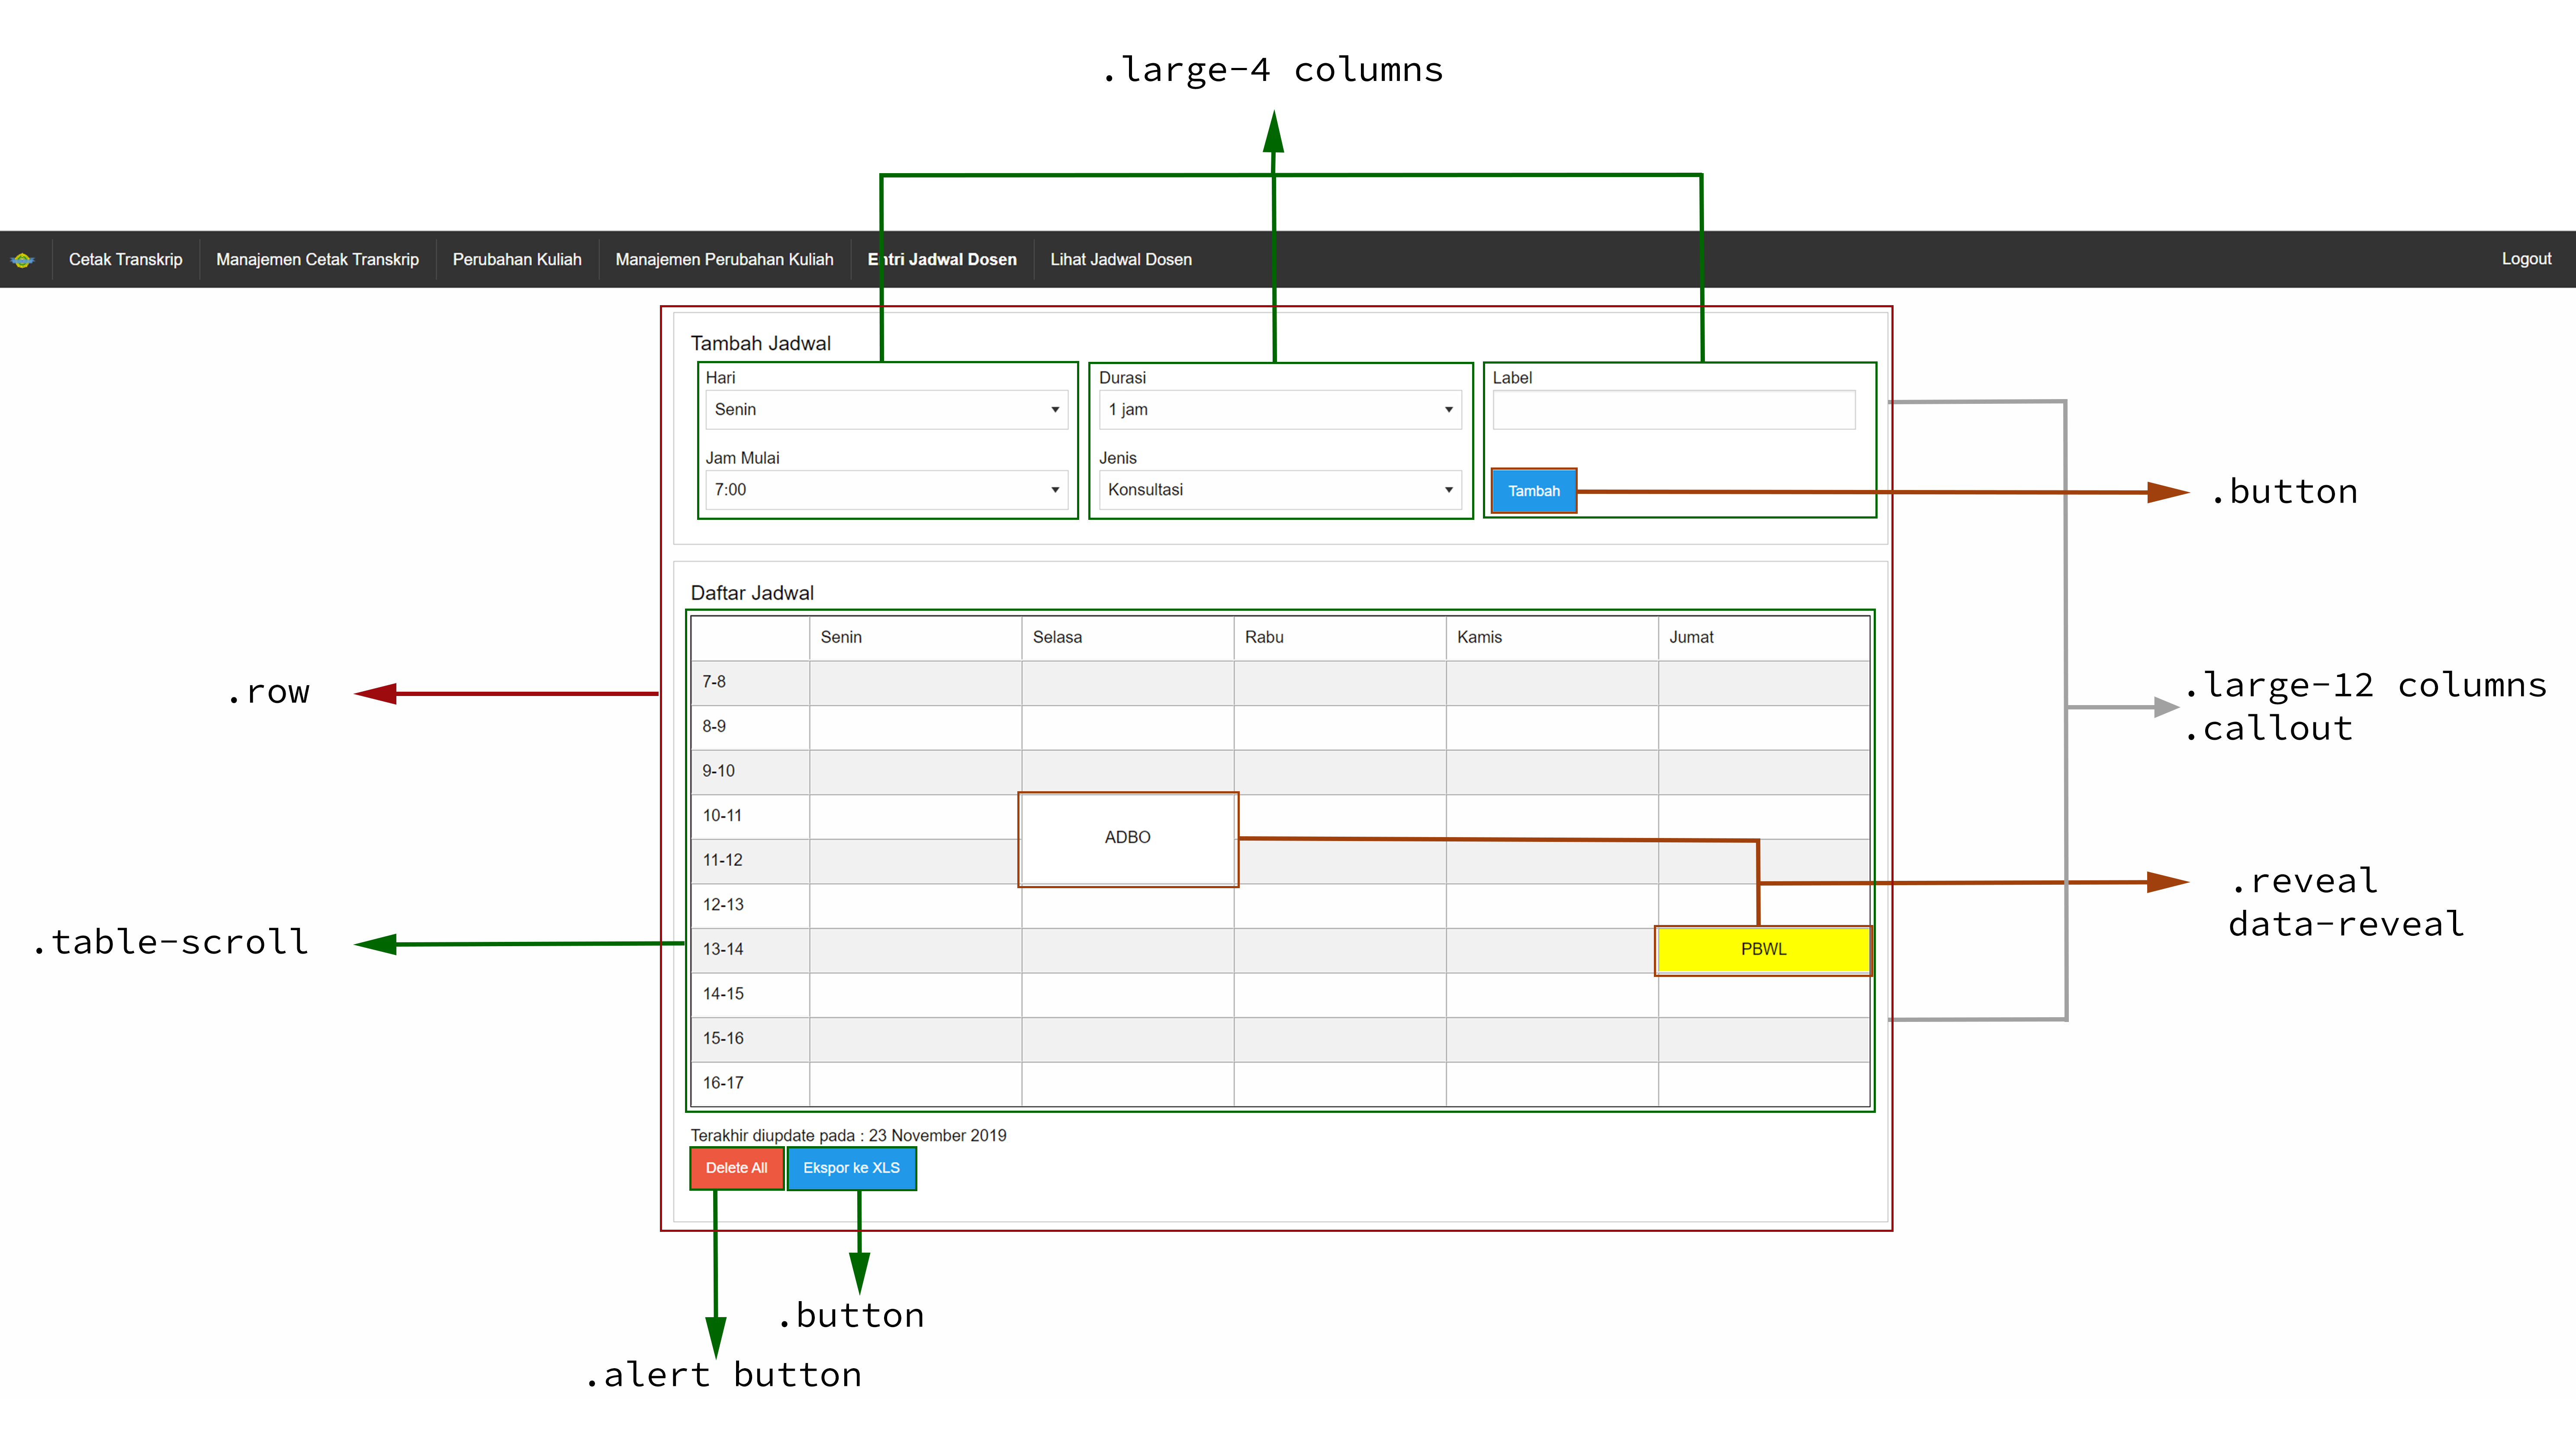
\includegraphics[width=\textwidth,height=\textheight,keepaspectratio]{foundation/analisis_tampilan_entri_jadwal_dosen.png}
	\caption{Analisis halaman entri jadwal dosen.}
	\label{fig:analisisEntriJadwalDosen}
\end{figure}

\noindent Gambar ~\ref{fig:konversiEntriJadwalDosen} menjelaskan komponen dalam website beserta penamaan kelas untuk Bootstrap 4 pada halaman entri jadwal dosen.\\
\begin{figure} [H]
	\centering  
	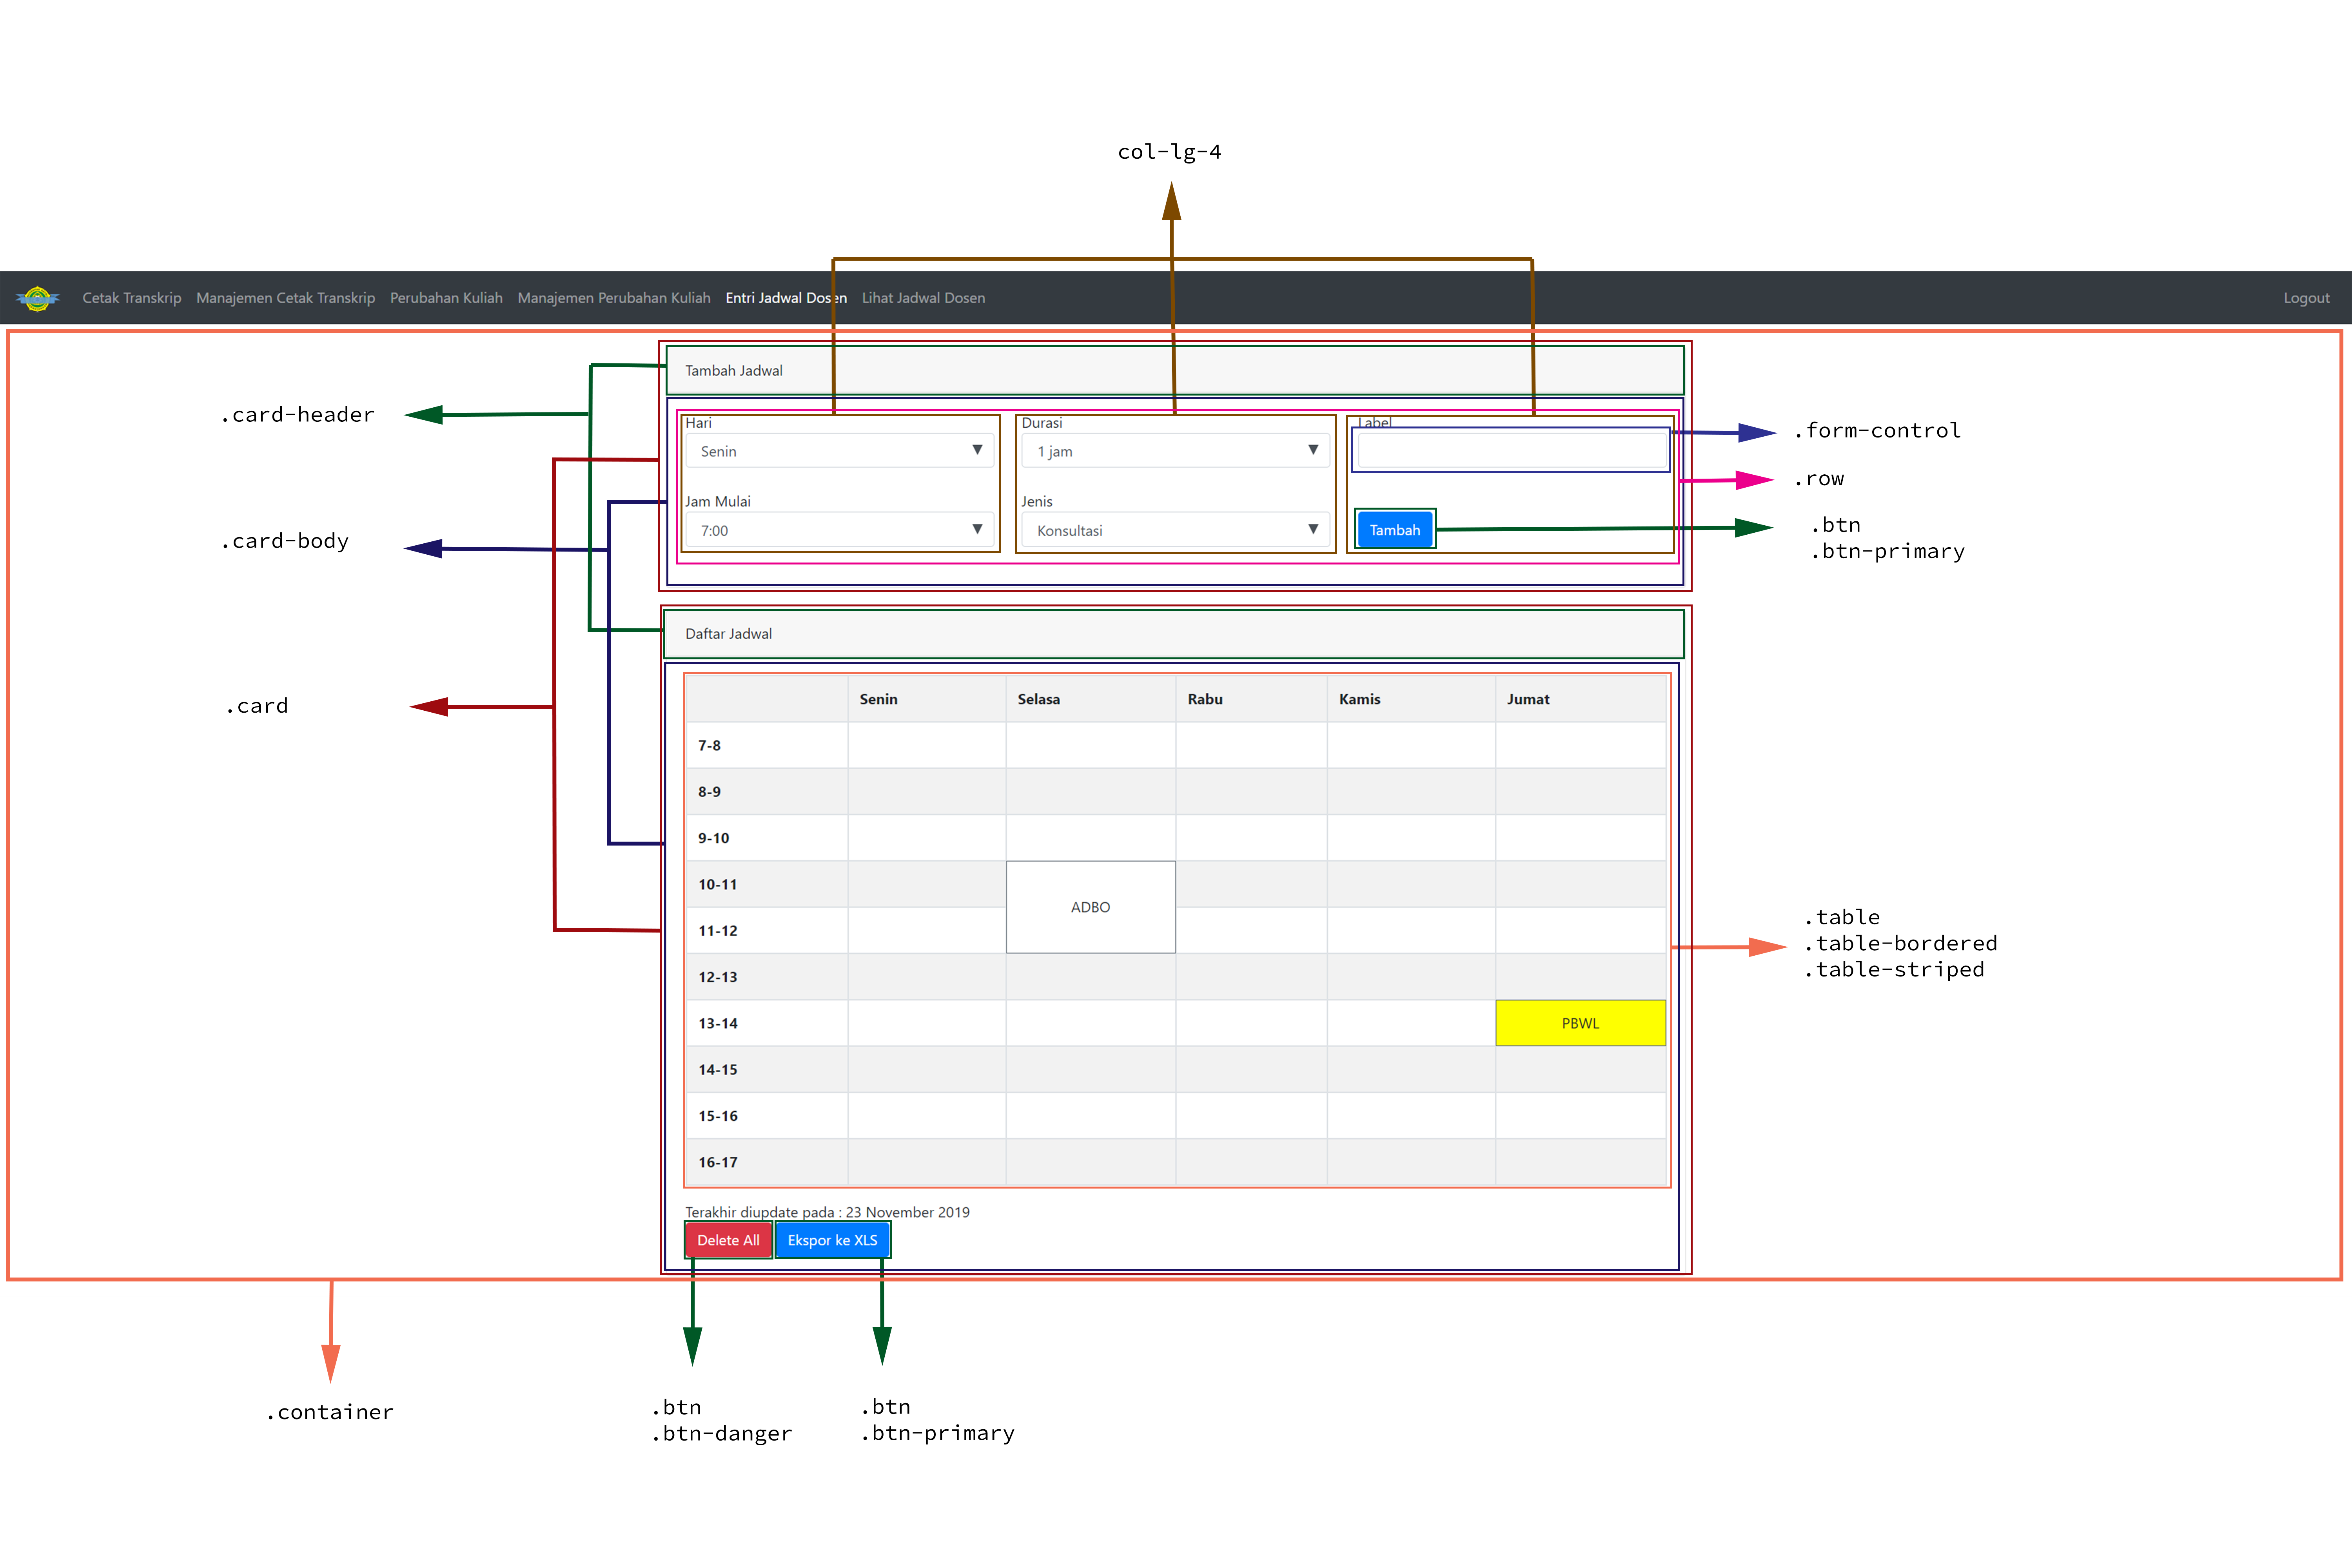
\includegraphics[width=\textwidth,height=\textheight,keepaspectratio]{bootstrap/konversi_tampilan_entri_jadwal_dosen.png}
	\caption{Konversi halaman entri jadwal dosen.}
	\label{fig:konversiEntriJadwalDosen}
\end{figure}

Kode ~\ref{lst:mainEntriJadwalDosen} menjabarkan perubahan halaman entri jadwal dosen:
\begin{lstlisting}[language=diff, caption=Kode untuk Halaman Entri Jadwal Dosen,  basicstyle=\ttfamily, frame=single,
columns=fullflexible, keepspaces=true, breaklines=true, label={lst:mainEntriJadwalDosen}]
diff -r a\www\application\views\EntriJadwalDosen\main.php b\www\application\views\EntriJadwalDosen\main.php
66c72
< <td style='width:10%'></td>
---
> <th></th>

69c75
< echo "<td style='width:18%'> $namaHari[$i] </td>"; //Membuat Header Tabel yang berisi daftar hari
---
> echo "<th> $namaHari[$i] </th>"; //Membuat Header Tabel yang berisi daftar hari

91a98
> $border = "border border-secondary align-middle";

106a114
> $($cellLocation).addClass('<?php echo $border; ?>');
\end{lstlisting}
Kode lengkap dari file ini dapat dilihat dalam lampiran ~\ref{lst:resentriJadwalDosen}.

Beberapa catatan dari kode diatas tertera pada tabel ~\ref{tabel:entriJadwalDosen}:
\begin{table}[H]
	\centering
	\caption{Penjelasan kode entri jadwal dosen.}
	\begin{tabularx}{\textwidth}{llX}
		\toprule
		No & Implementasi     & Penjelasan \\
		\midrule
		8, 10 & Perbaikan tabel & Tag \texttt{<td>} diubah menjadi \texttt{<th>} agar \textit{cell} yang terisi dapat memiliki border.\\
		13 & Kelas border & Pada Bootstrap 4 border terbentuk dengan memanfaatkan kelas \texttt{border border-secondary align-middle}.\\
		16 & Pemanggilan kelas border & Kelas border disimpan dalam variabel dan dipanggil ketika \textit{cell} terisi.\\
		\bottomrule
	\end{tabularx}%
	\label{tabel:entriJadwalDosen}
\end{table}

\subsection{Halaman	Lihat Jadwal Dosen}
\noindent Gambar ~\ref{fig:analisisLihatJadwalDosen} merupakan halaman lihat jadwal dosen berisi sebuah tabs, dimana setiap judul tabs yang berada diatas tabel mereferensikan ke \texttt{tabs-content} atau halaman jadwal setiap dosen. Kemudian pada bagian bawah tabel terdapat tombol biru "Ekspor ke XLS".
\begin{figure} [H]
	\centering  
	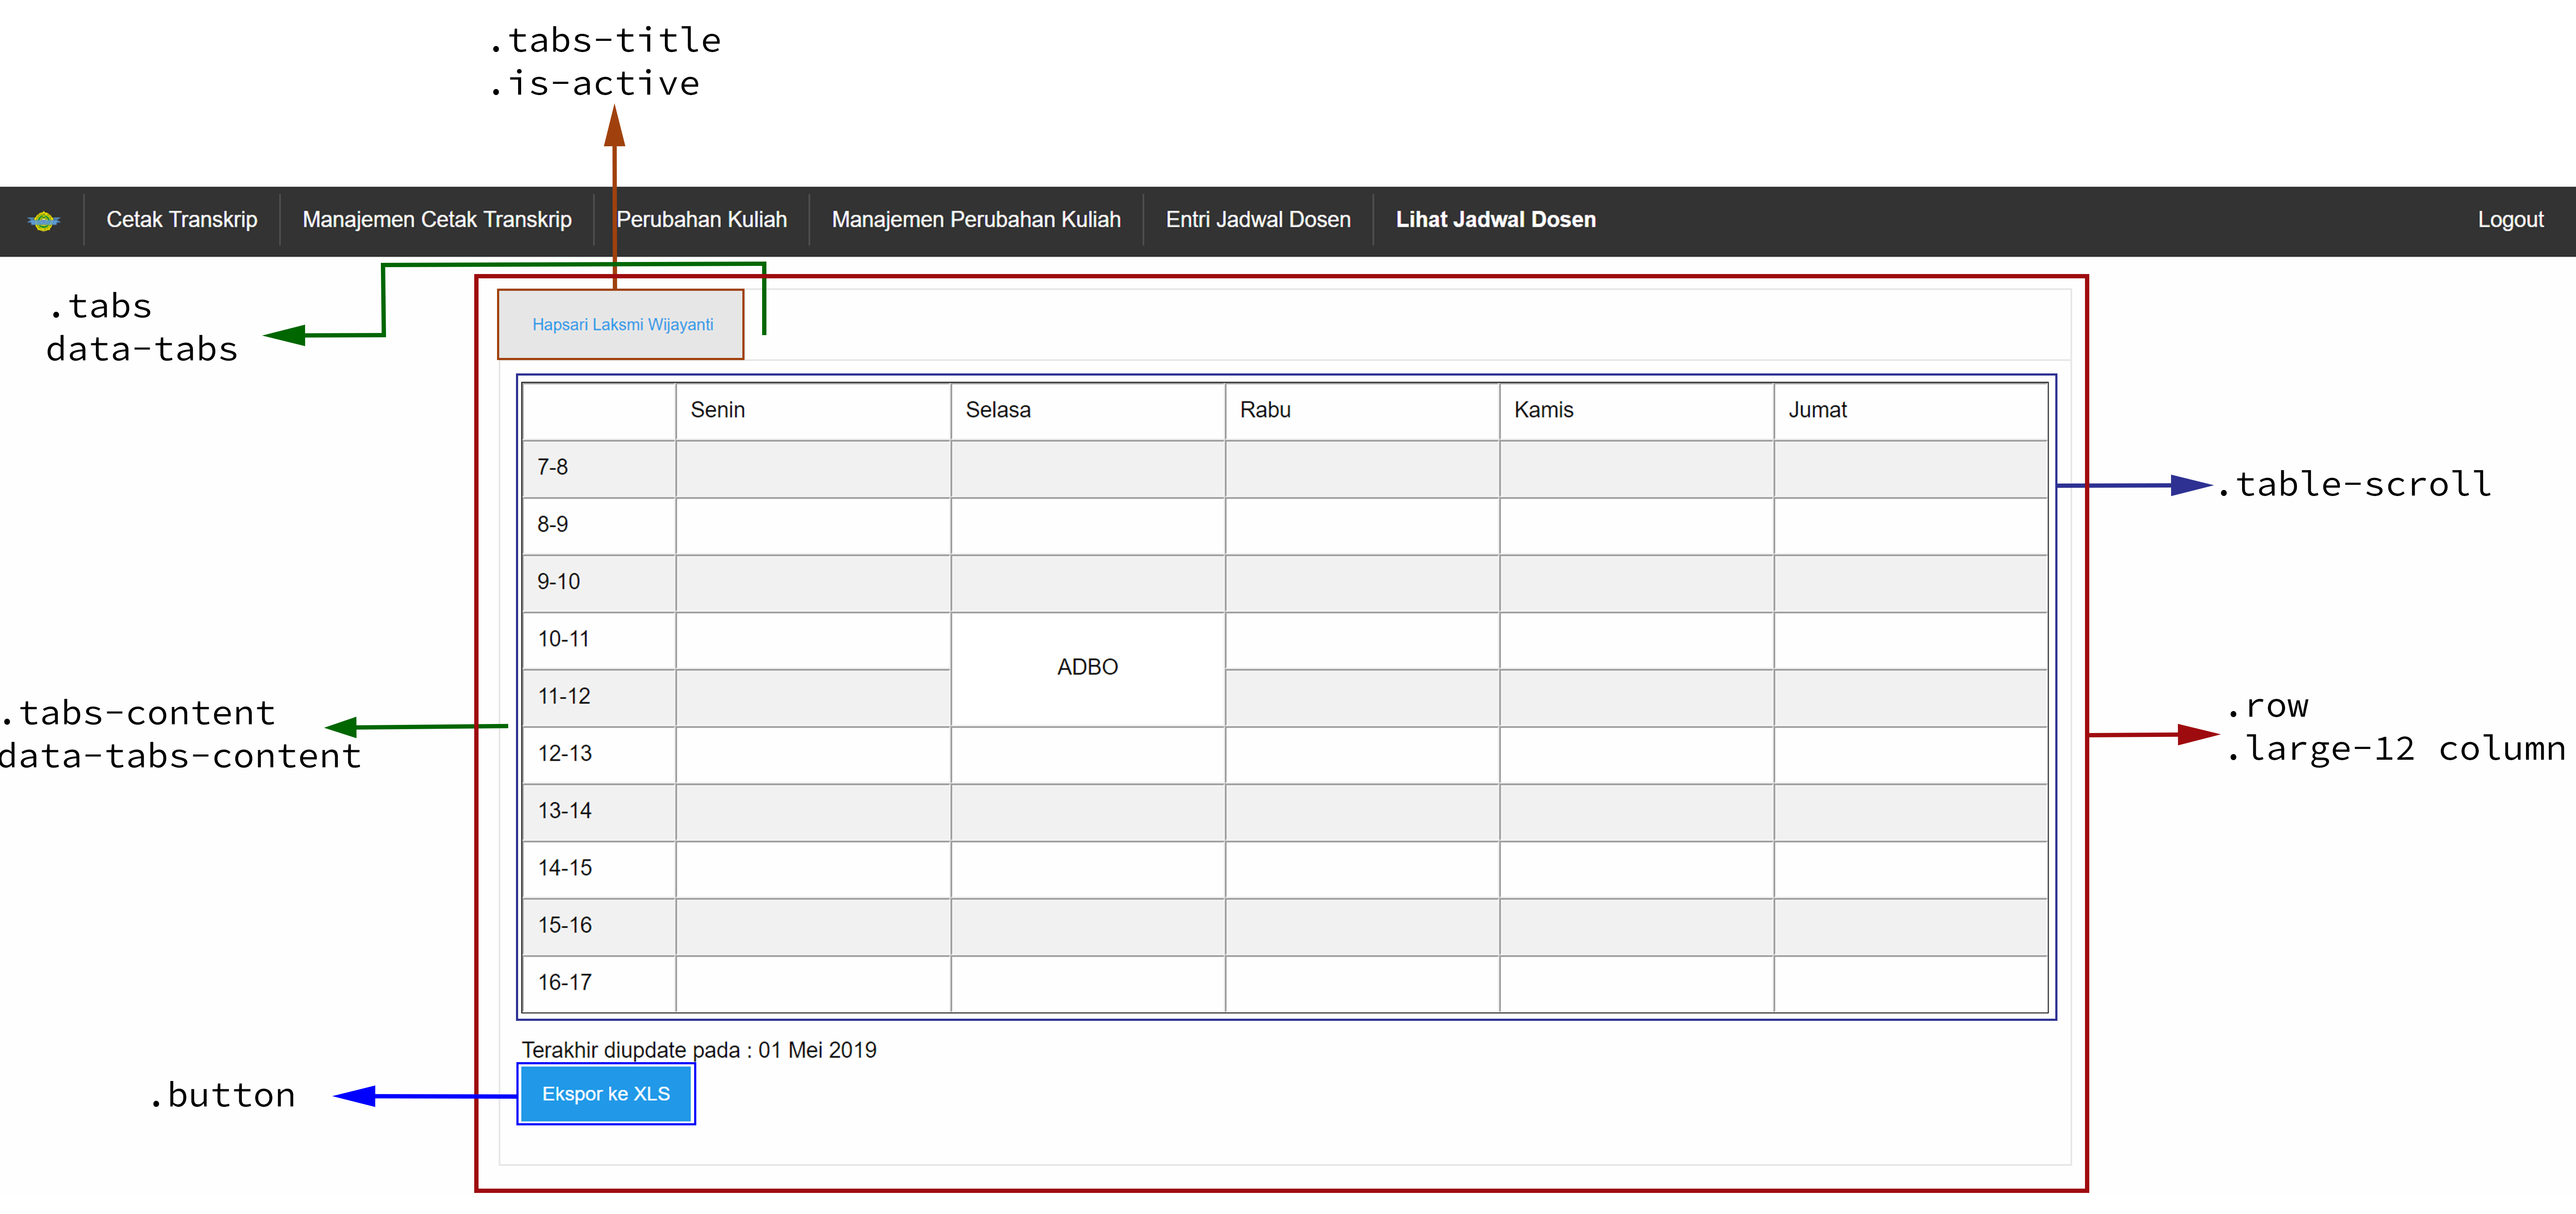
\includegraphics[width=\textwidth,height=\textheight,keepaspectratio]{foundation/analisis_tampilan_lihat_jadwal_dosen.png}
	\caption{Analisis halaman lihat jadwal dosen.}
	\label{fig:analisisLihatJadwalDosen}
\end{figure}

\noindent Gambar ~\ref{fig:konversiLihatJadwalDosen} menjelaskan komponen dalam website beserta penamaan kelas untuk Bootstrap 4 pada halaman lihat jadwal dosen.\\

\begin{figure} [H]
	\centering  
	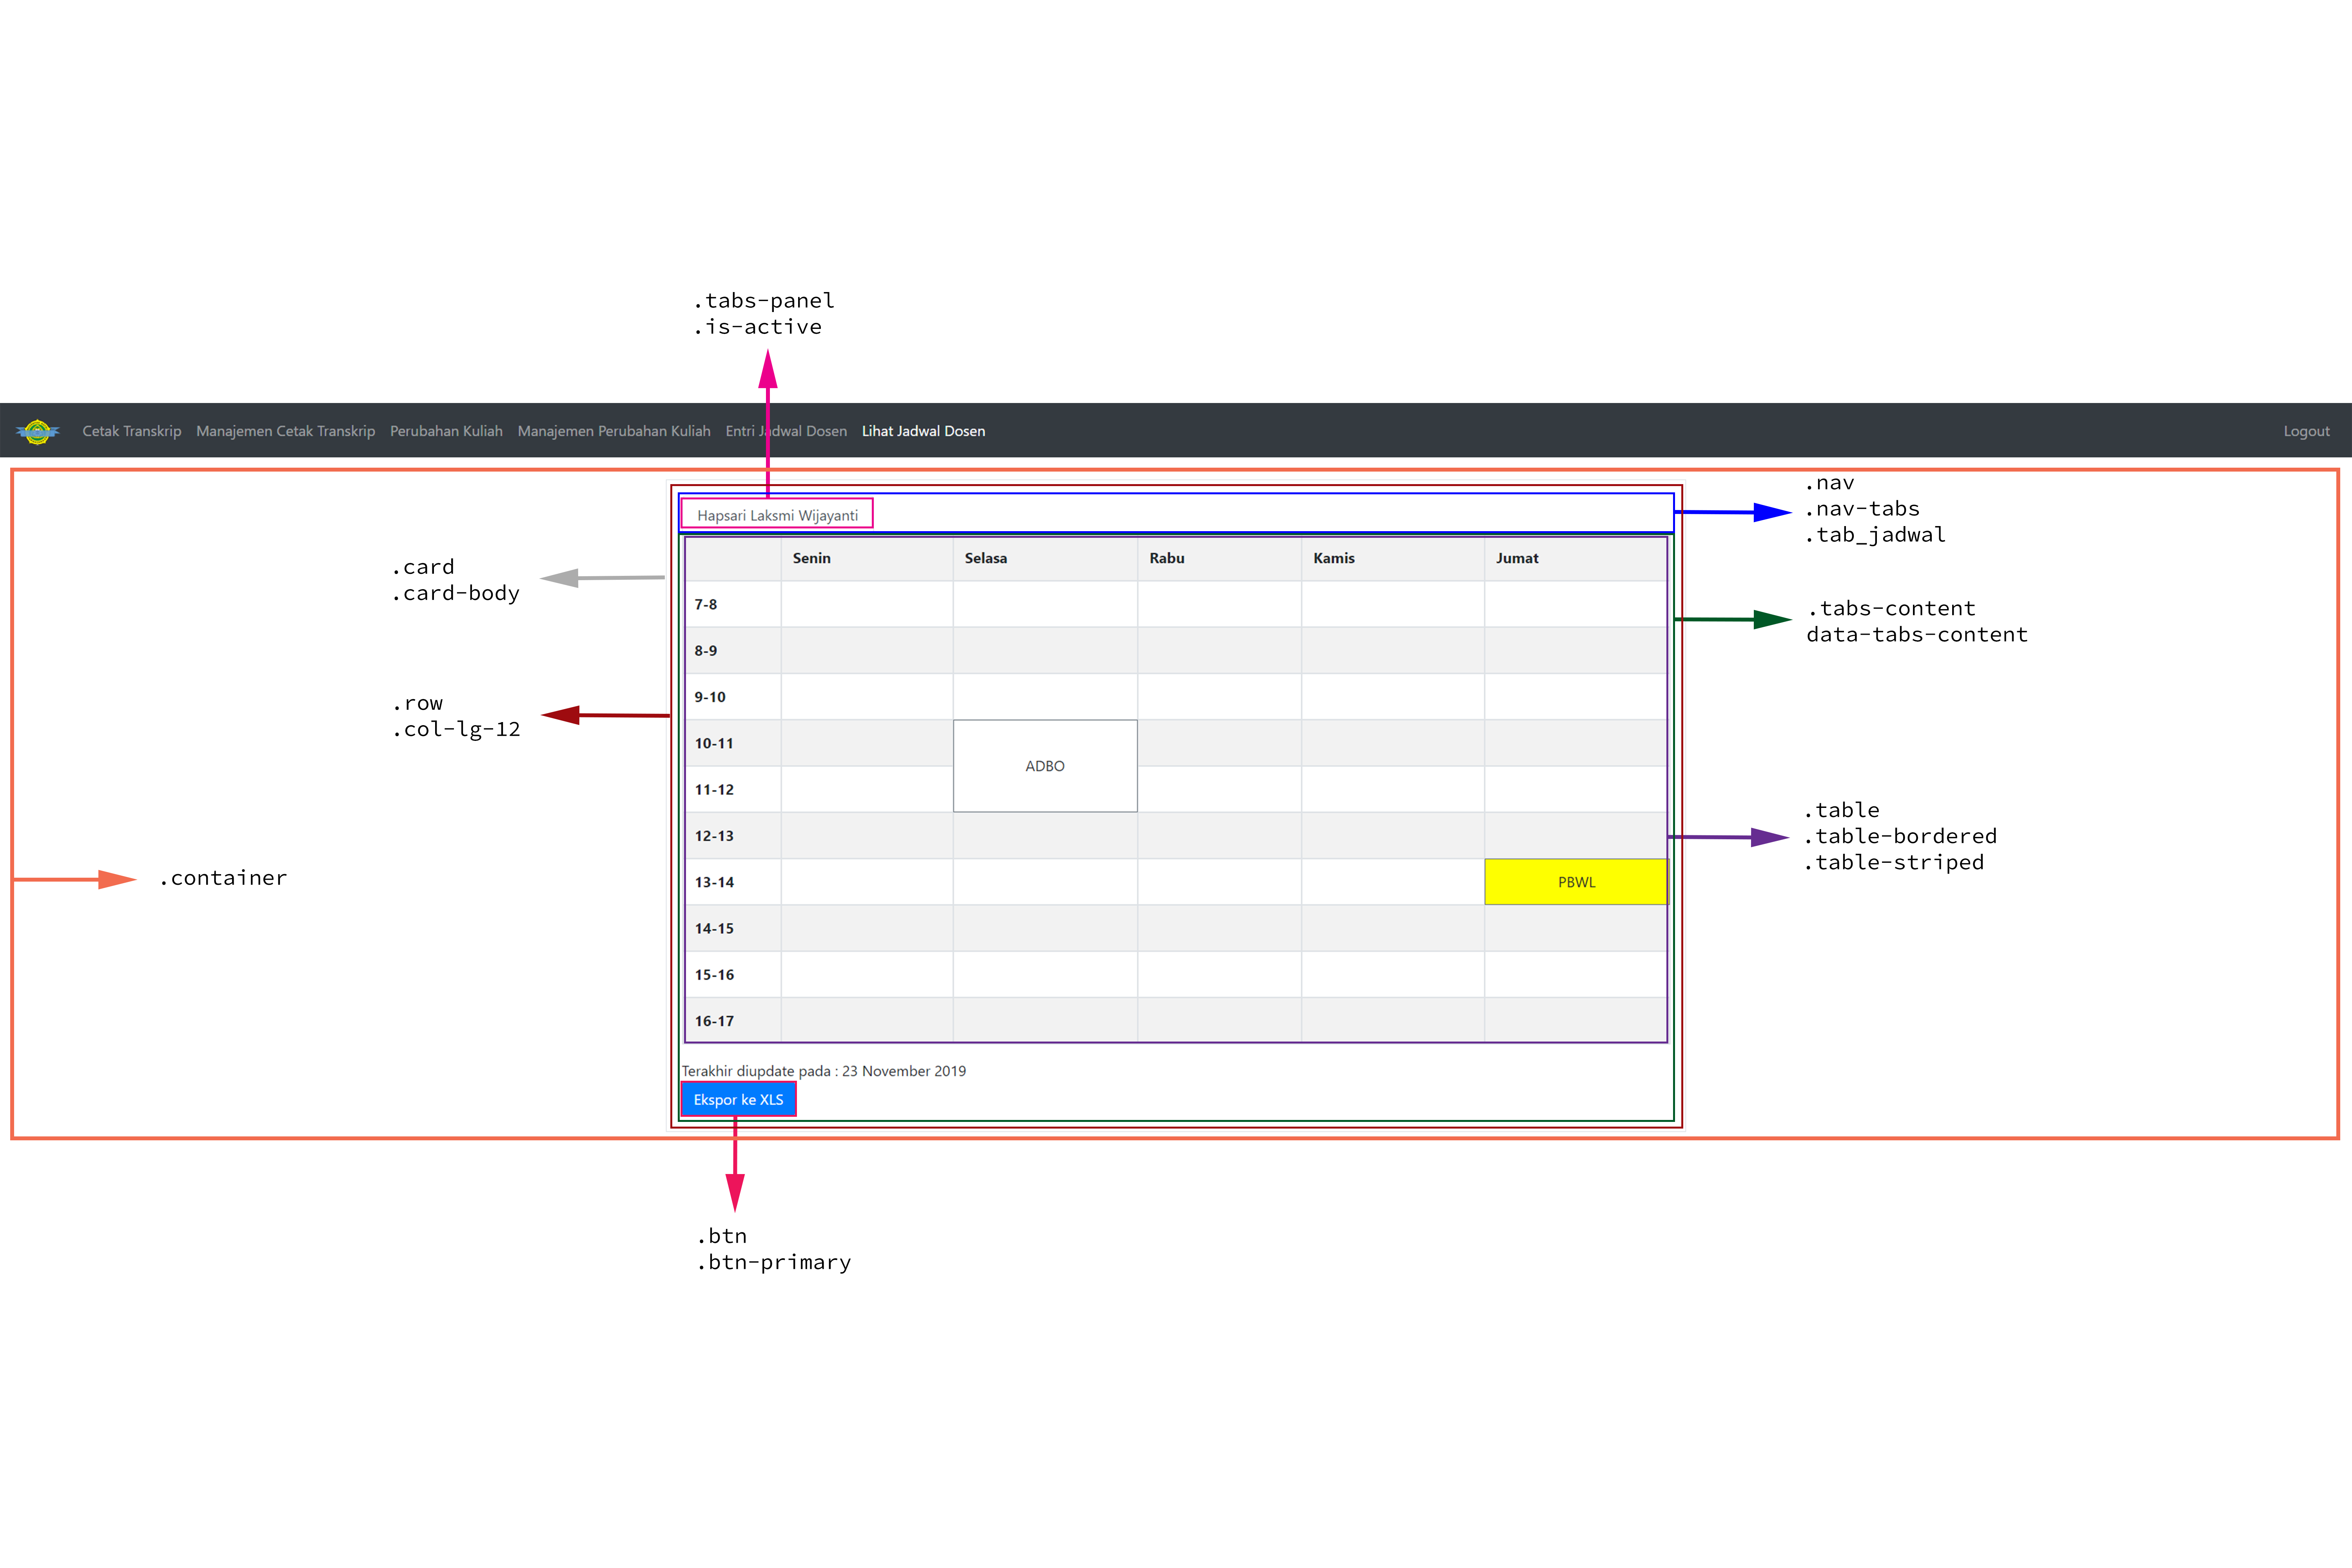
\includegraphics[width=\textwidth,height=\textheight,keepaspectratio]{bootstrap/konversi_lihat_jadwal_dosen.png}
	\caption{Konversi modal lihat jadwal dosen.}
	\label{fig:konversiLihatJadwalDosen}
\end{figure}
Kode ~\ref{lst:mainLihatJadwalDosen} menjabarkan perubahan halaman lihat jadwal dosen:
\begin{lstlisting}[language=diff, caption=Kode untuk Halaman Lihat Jadwal Dosen,  basicstyle=\ttfamily, frame=single,
columns=fullflexible, keepspaces=true, breaklines=true, label={lst:mainLihatJadwalDosen}]
diff -r a\www\application\views\LihatJadwalDosen\main.php b\www\application\views\LihatJadwalDosen\main.php

22c22
< <li class="tabs-title is-active"><a href="#hal<?php echo $idx; ?>" aria-selected="true"><?php foreach ($currRow as $data) {
---
> <li class="nav-item"><a class="nav-link active" href="#hal<?php echo $idx; ?>" aria-selected="true"><?php foreach ($currRow as $data) {

29c29
< <li class="tabs-title"><a a href="#hal<?php echo $idx; ?>"><?php foreach ($currRow as $data) {
---
> <li class="nav-item"><a class="nav-link" href="#hal<?php echo $idx; ?>"><?php foreach ($currRow as $data) {
\end{lstlisting}
Kode lengkap dari file ini dapat dilihat dalam lampiran ~\ref{lst:reslihatJadwalDosen}.

Keterangan dari kode diatas tertera pada tabel ~\ref{tabel:lihatJadwalDosen}:
\begin{table}[H]
	\centering
	\caption{Penjelasan kode lihat jadwal dosen}
	\begin{tabularx}{\textwidth}{llX}
		\toprule
		No & Implementasi     & Penjelasan \\
		\midrule
		3-11 & \textbf{Tabs}  & Tabs pada Foundation 6 dan Bootstrap 4 hanya berbeda penamaan nya saja.\\
		\bottomrule
	\end{tabularx}%
	\label{tabel:lihatJadwalDosen}
\end{table}

\subsection{Kotak Dialog/Modal}
\subsubsection{Modal}
Apabila user memilih salah satu ikon dari kolom 'Aksi' maka modal akan muncul. Terdapat lima macam modal yaitu: modal lihat, modal setuju, modal tolak, modal print dan modal hapus perubahan kuliah. 
Berikut ini gambar ~\ref{fig:analisisModalManajemenPerubahanKuliah} modal yang ada pada halaman manajemen perubahan kuliah dengan menggunakan Foundation 6.
\begin{figure} [H]	
	\centering
	\begin{subfigure}[b]{0.45\linewidth} 
		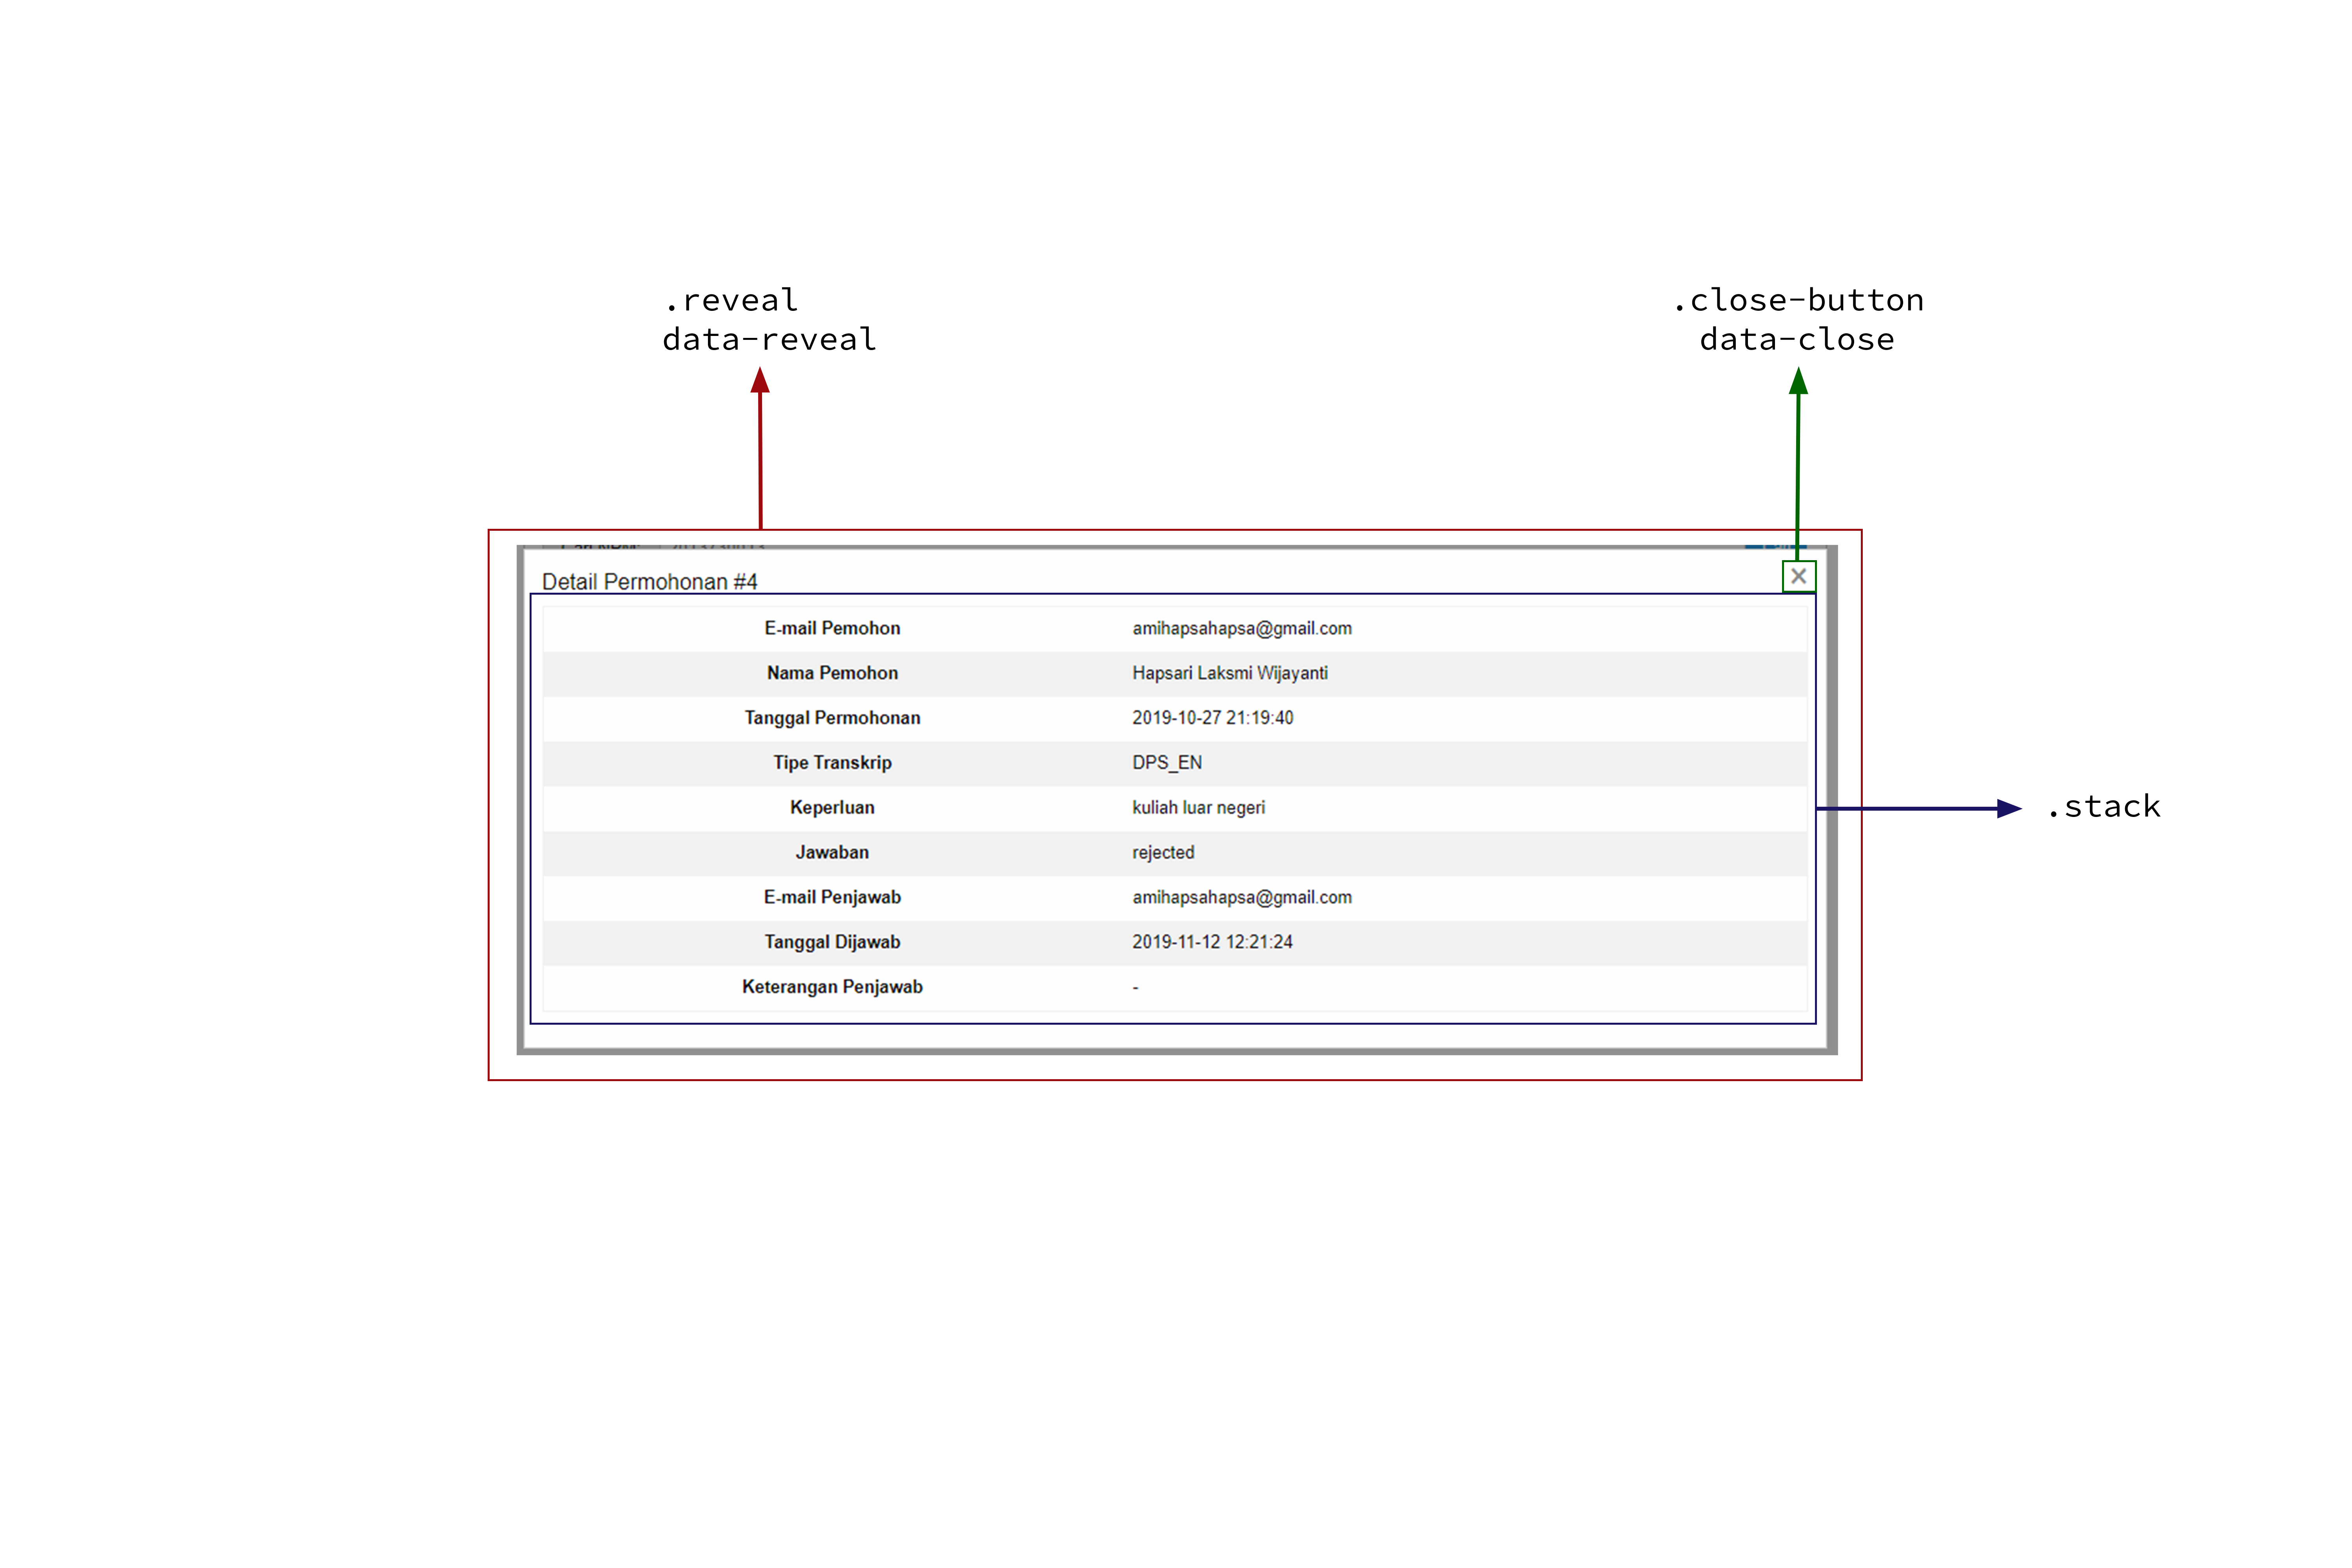
\includegraphics[width=\textwidth,height=\textheight,keepaspectratio]{foundation/analisis_modal_eye_manajemen_perubahan_kuliah.png}
		\caption{Modal lihat.}  
	\end{subfigure}	
	\begin{subfigure}[b]{0.3\linewidth}   
		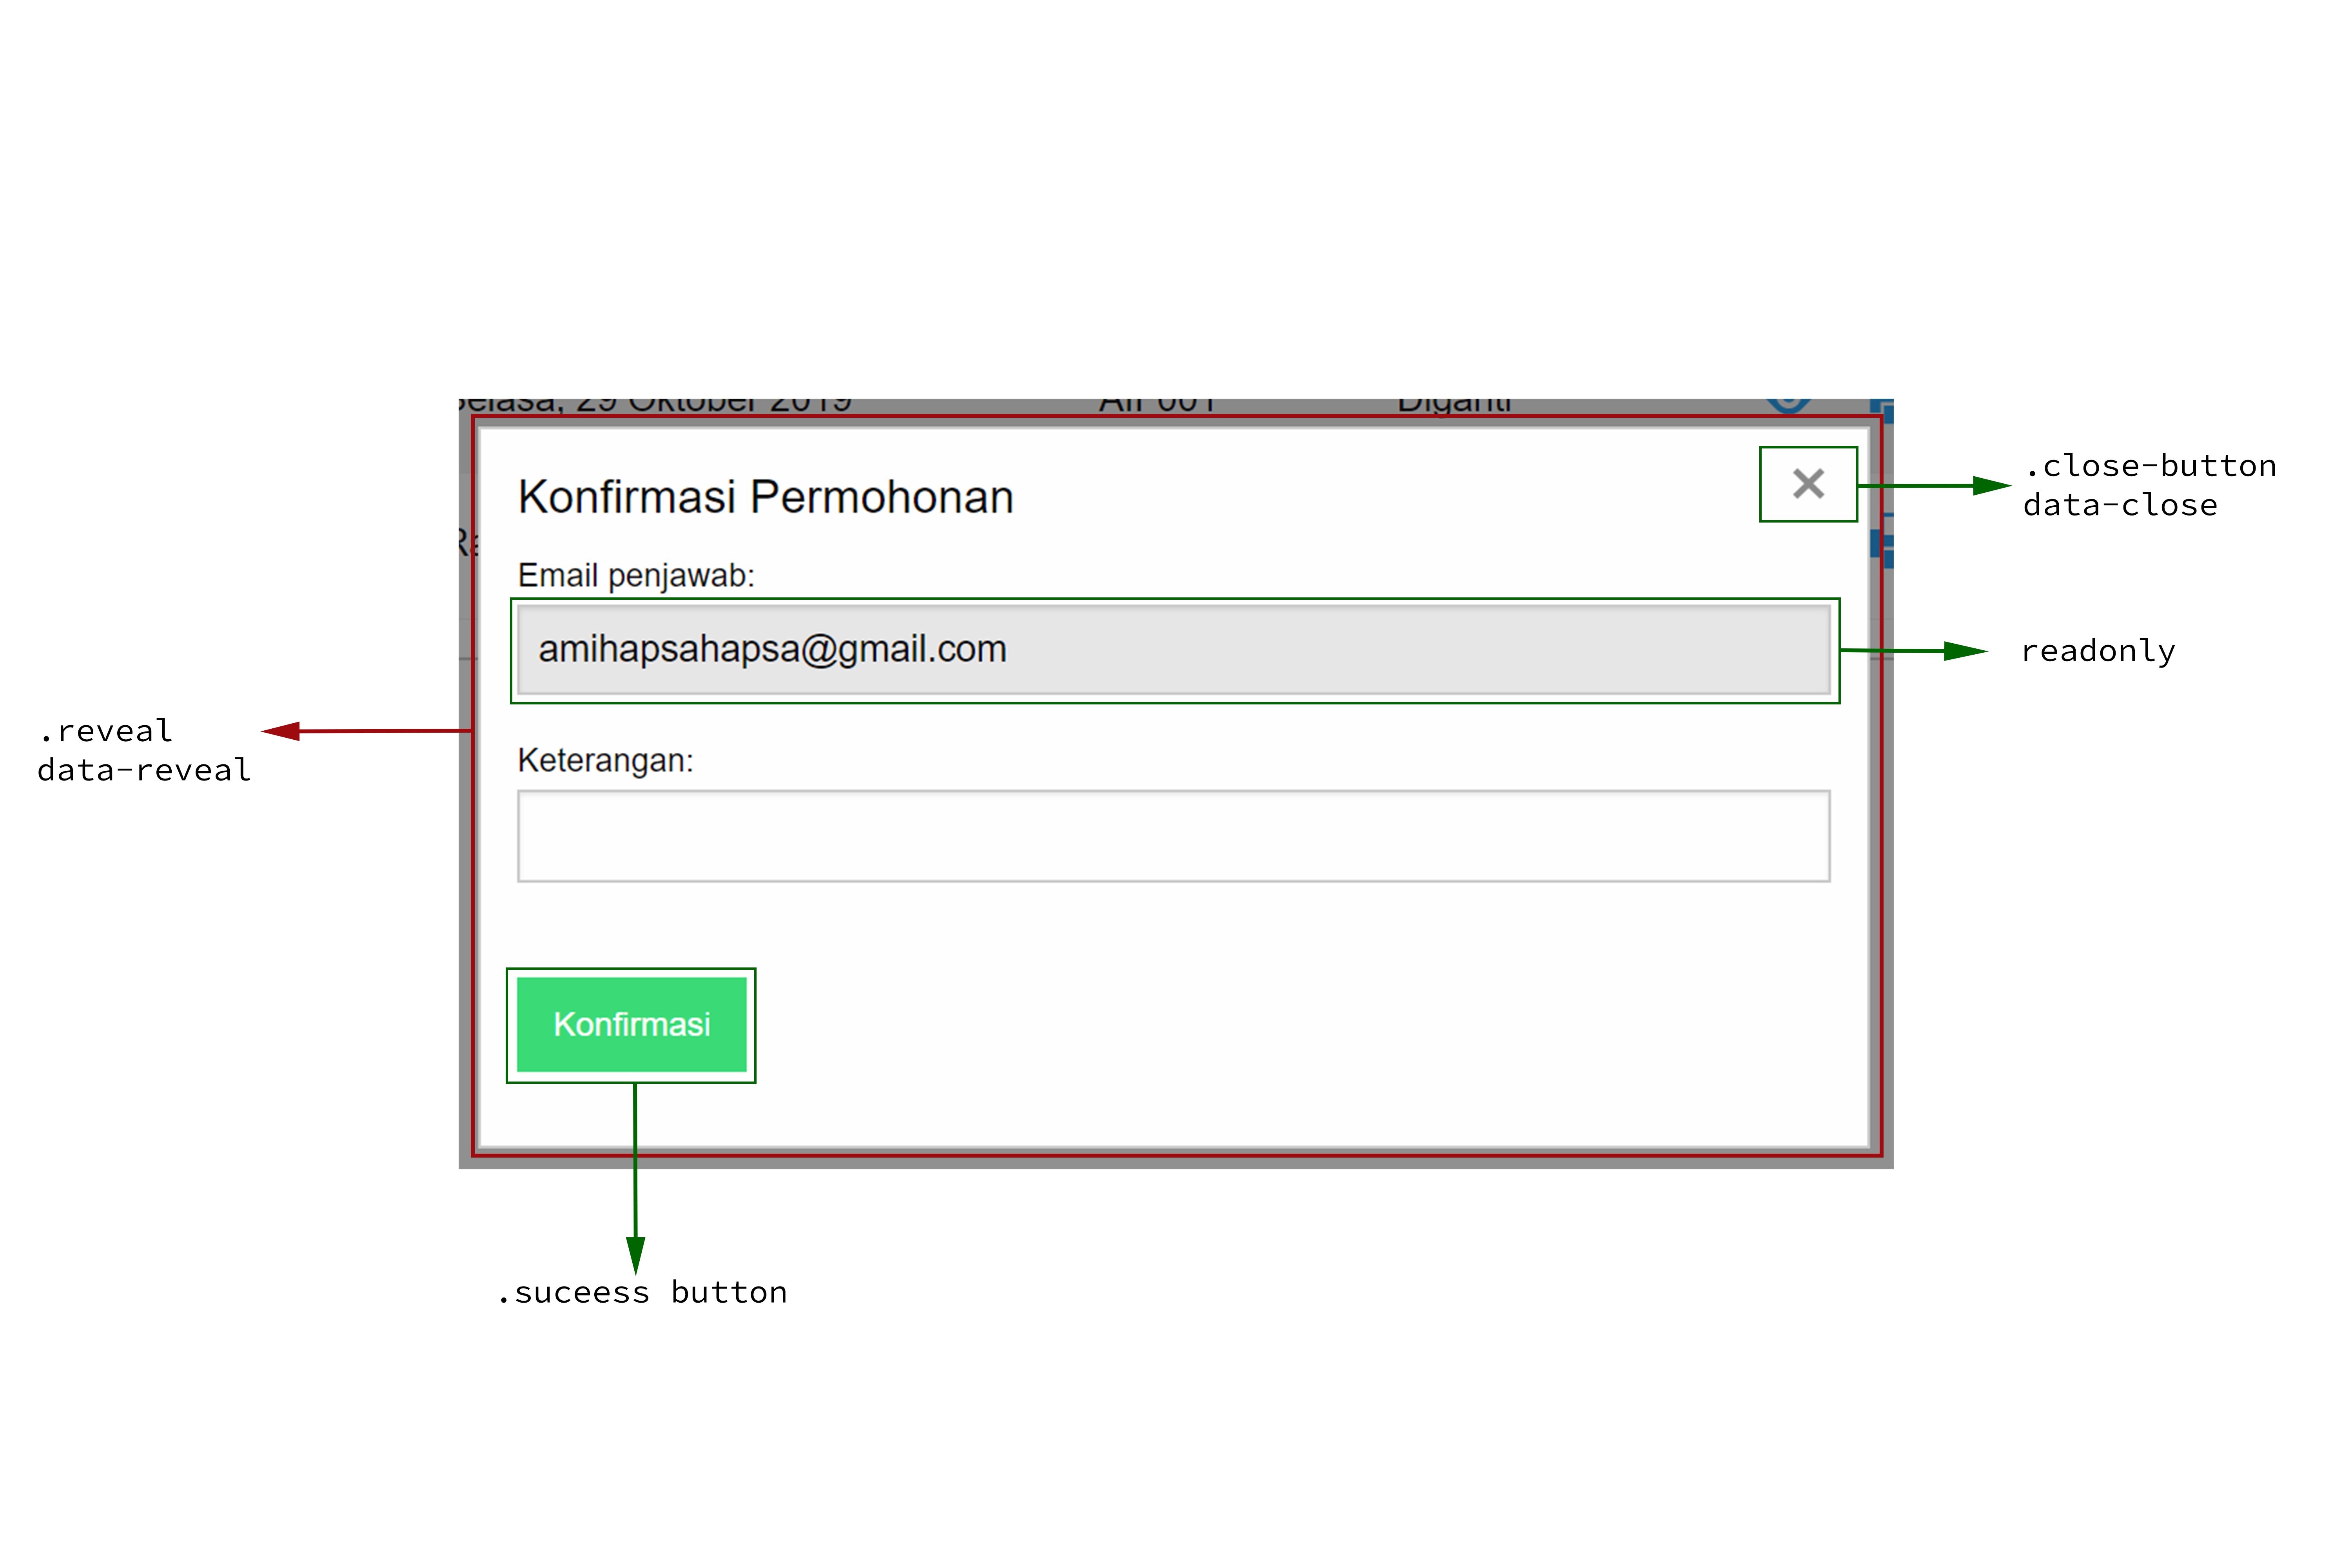
\includegraphics[width=\textwidth,height=\textheight,keepaspectratio]{foundation/analisis_modal_like_manajemen_perubahan_kuliah.png}
		\caption{Modal setuju.}
	\end{subfigure}
\end{figure}

\begin{figure} [H] 
	\centering
	\ContinuedFloat
	\begin{subfigure}[b]{0.6\linewidth}
		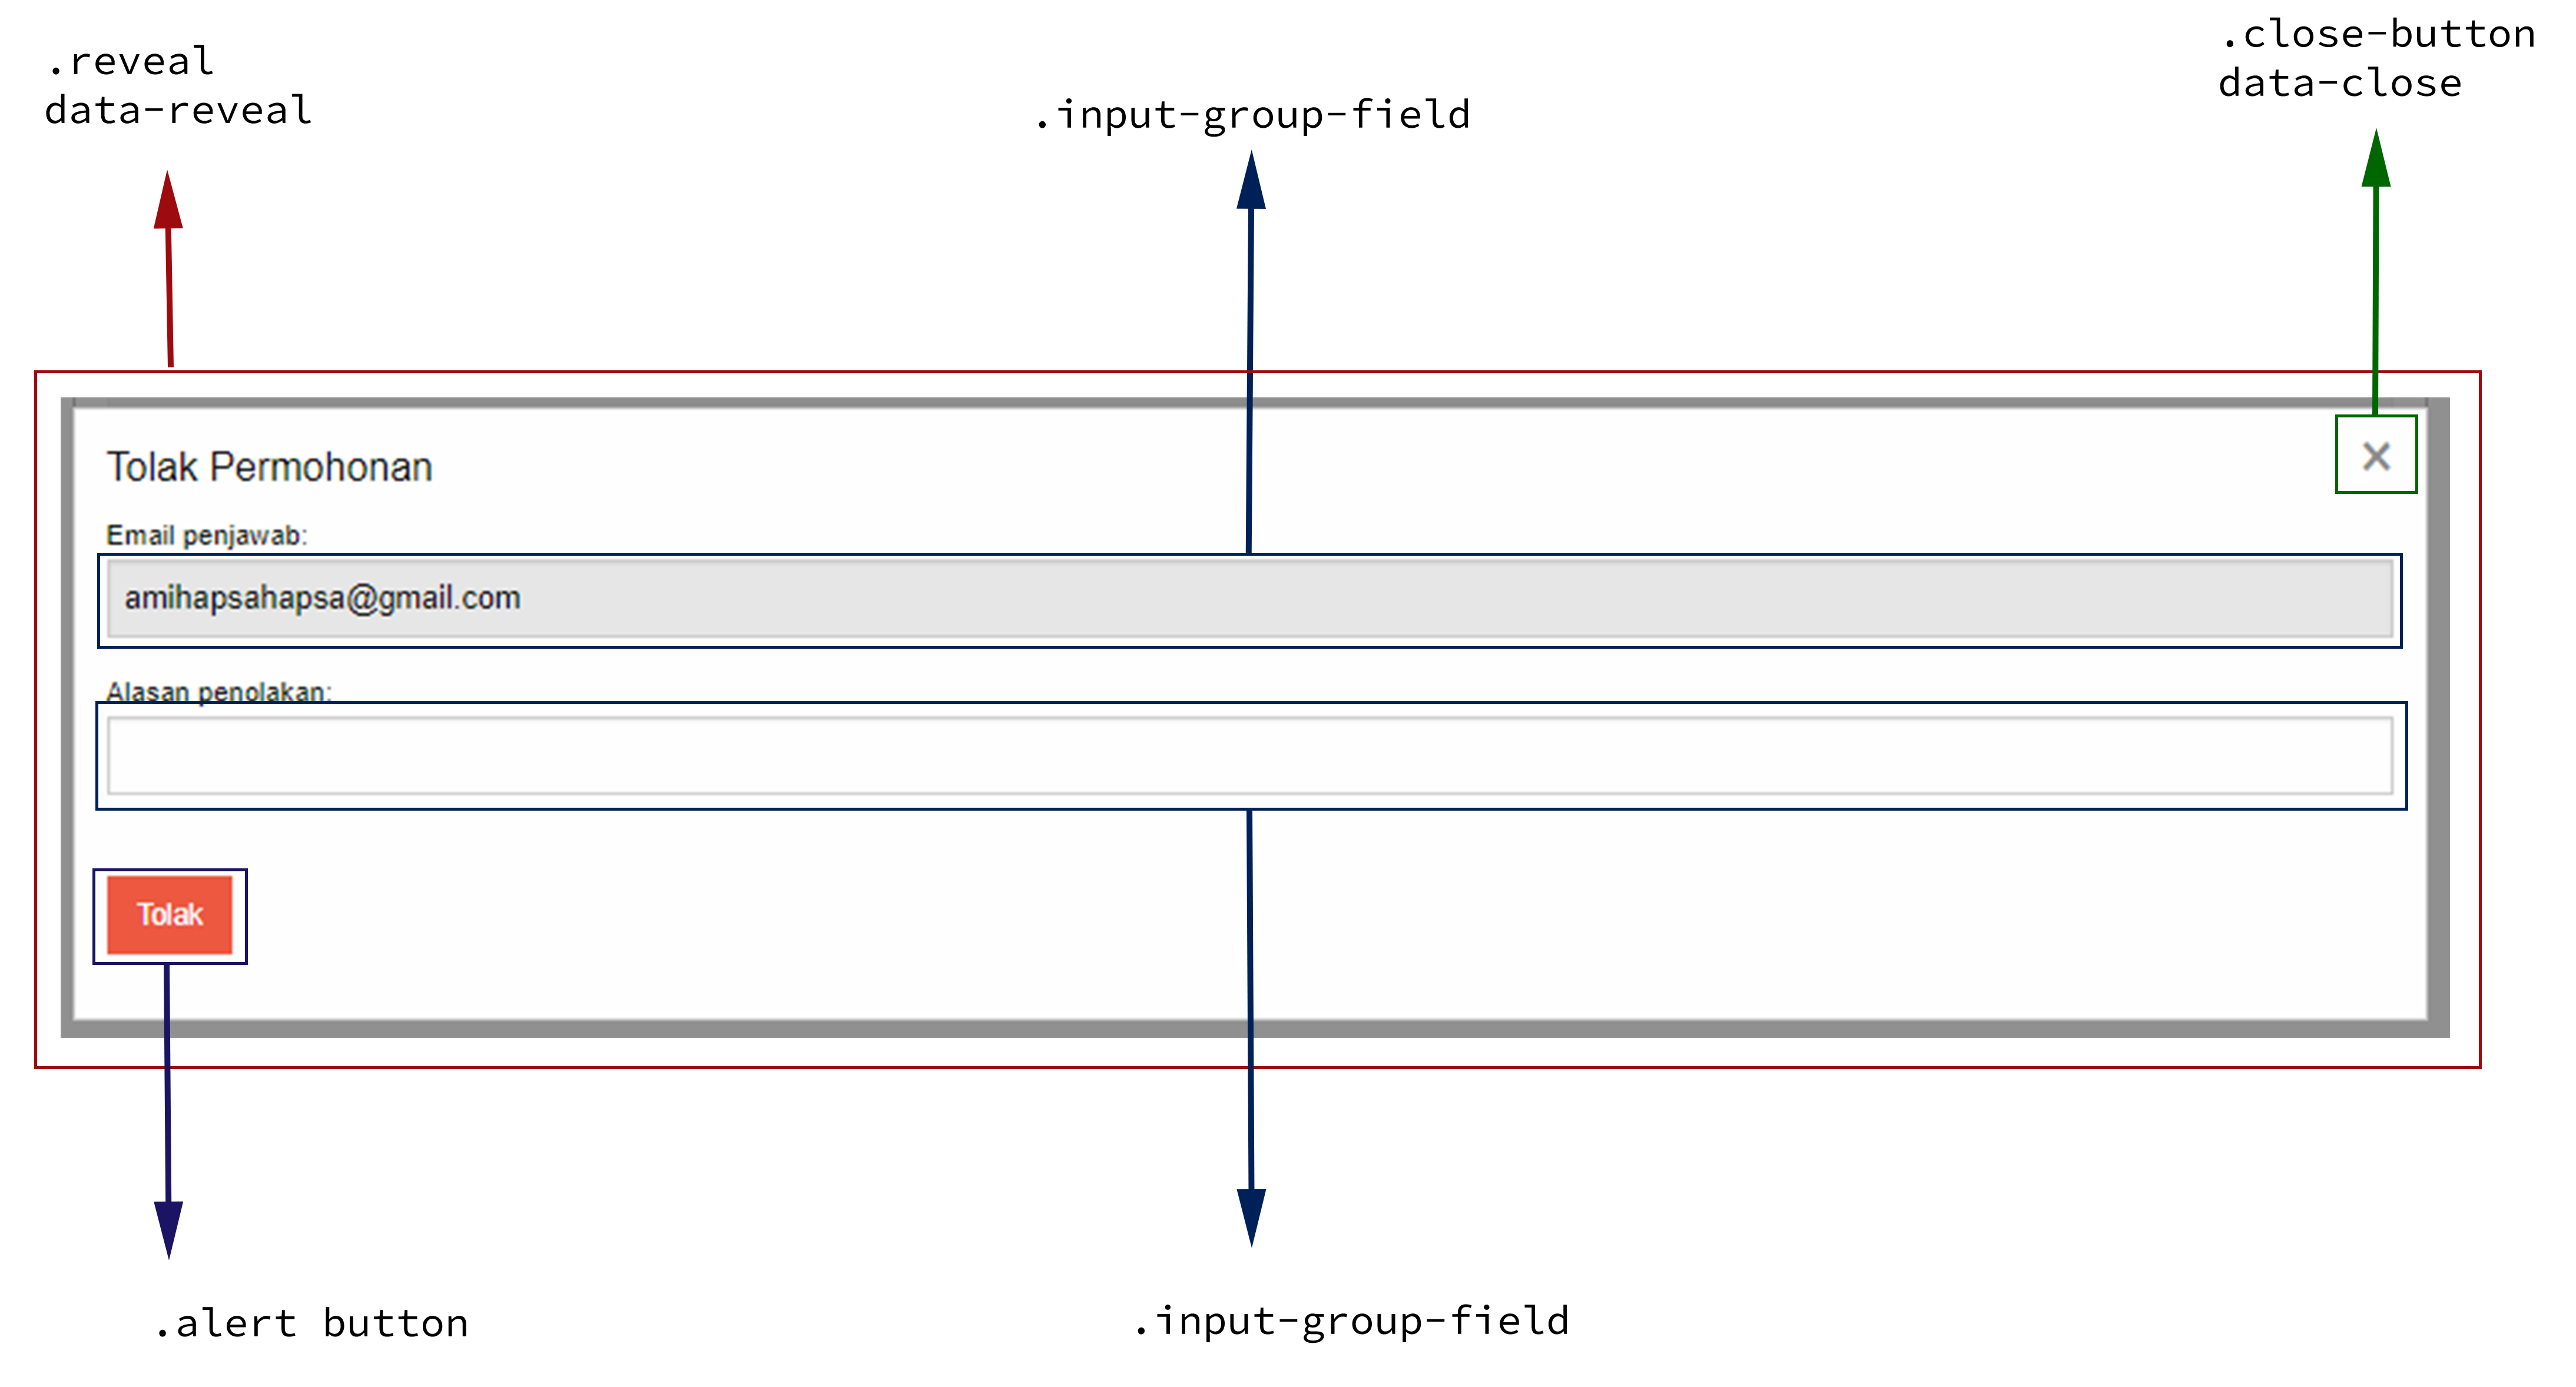
\includegraphics[width=\textwidth,height=\textheight,keepaspectratio]{foundation/analisis_modal_dislike_manajemen_perubahan_kuliah.png}
		\caption{Modal tolak.}  
	\end{subfigure}
\end{figure}

\begin{figure} [H] 
	\centering
	\ContinuedFloat
	\begin{subfigure}[b]{0.35\linewidth} 
		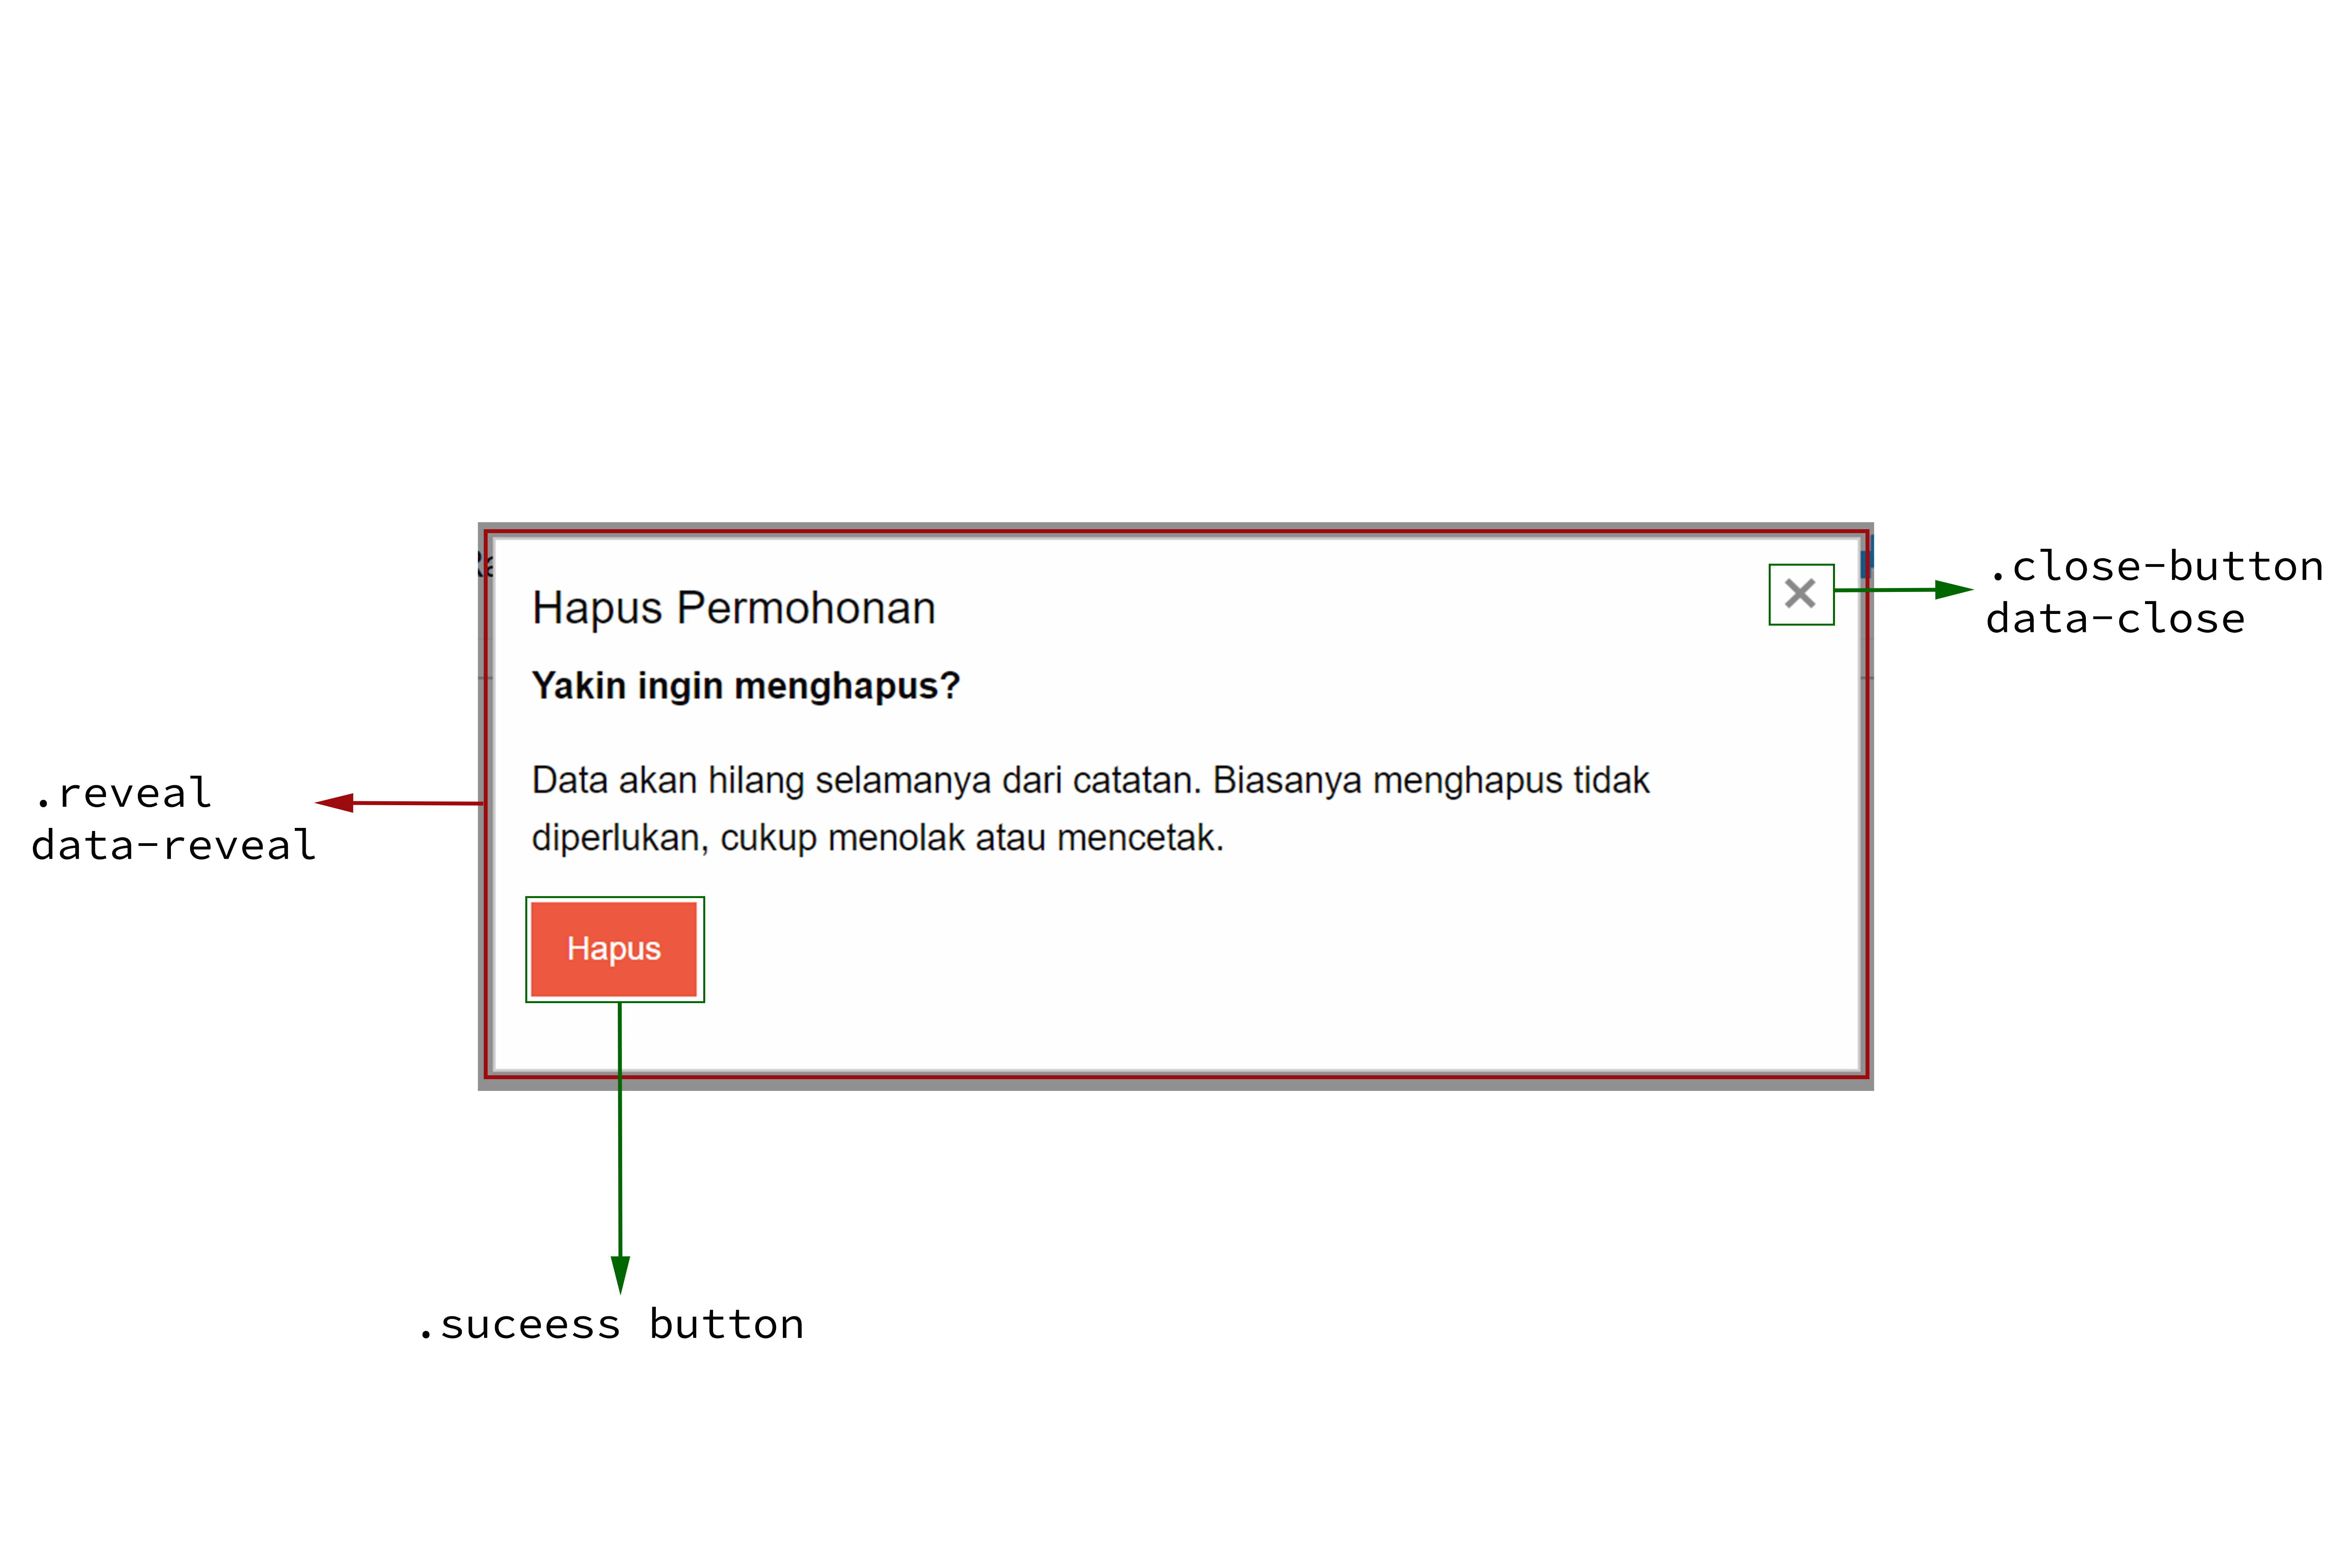
\includegraphics[width=\textwidth,height=\textheight,keepaspectratio]{foundation/analisis_modal_trash_manajemen_perubahan_kuliah.png}
		\caption{Modal hapus.}
	\end{subfigure}
	\begin{subfigure}[b]{0.55\linewidth}
		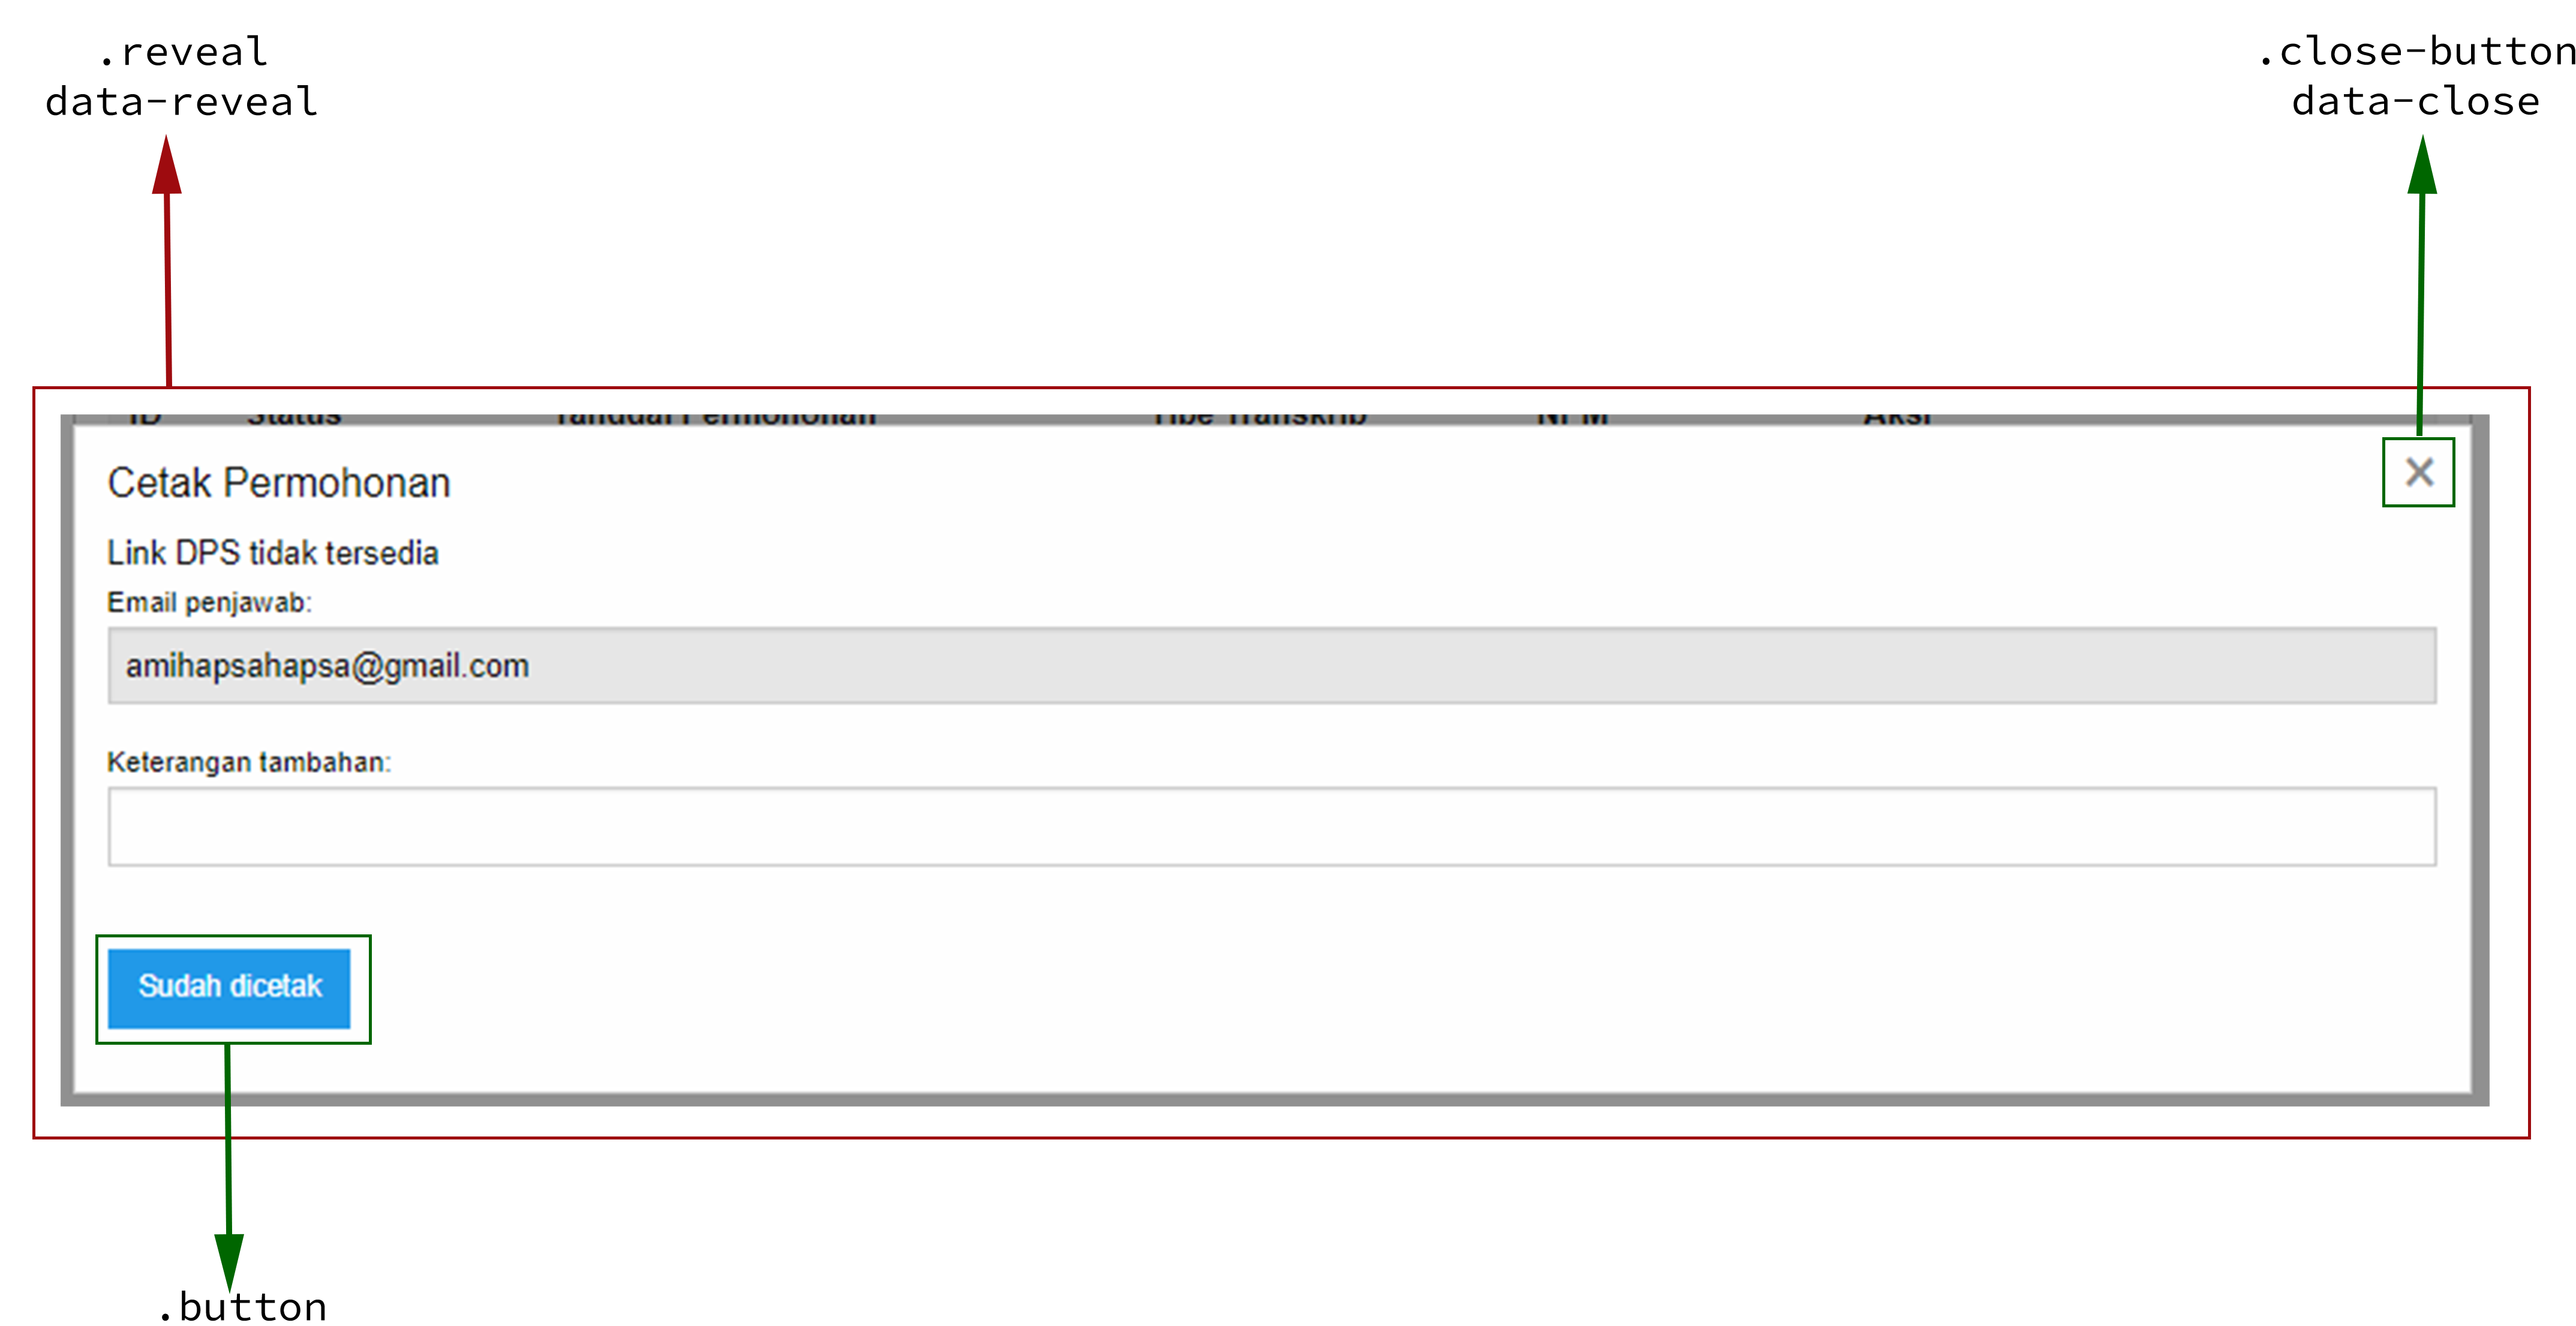
\includegraphics[width=\textwidth,height=\textheight,keepaspectratio]{foundation/analisis_modal_print_manajemen_cetak_transkrip.png}
		\caption{Modal print.}  
	\end{subfigure}	 
	\caption{Analisis modal pada halaman manajemen perubahan kuliah.}
	\label{fig:analisisModalManajemenPerubahanKuliah}
\end{figure}

\noindent Gambar ~\ref{fig:konversiModalManajemenPerubahanKuliah} menjelaskan komponen dalam website beserta penamaan kelas untuk Bootstrap 4 pada halaman modal manajemen perubahan kuliah.\\
\begin{figure}[H]
	\centering
	\begin{subfigure}[b]{0.45\linewidth} 
		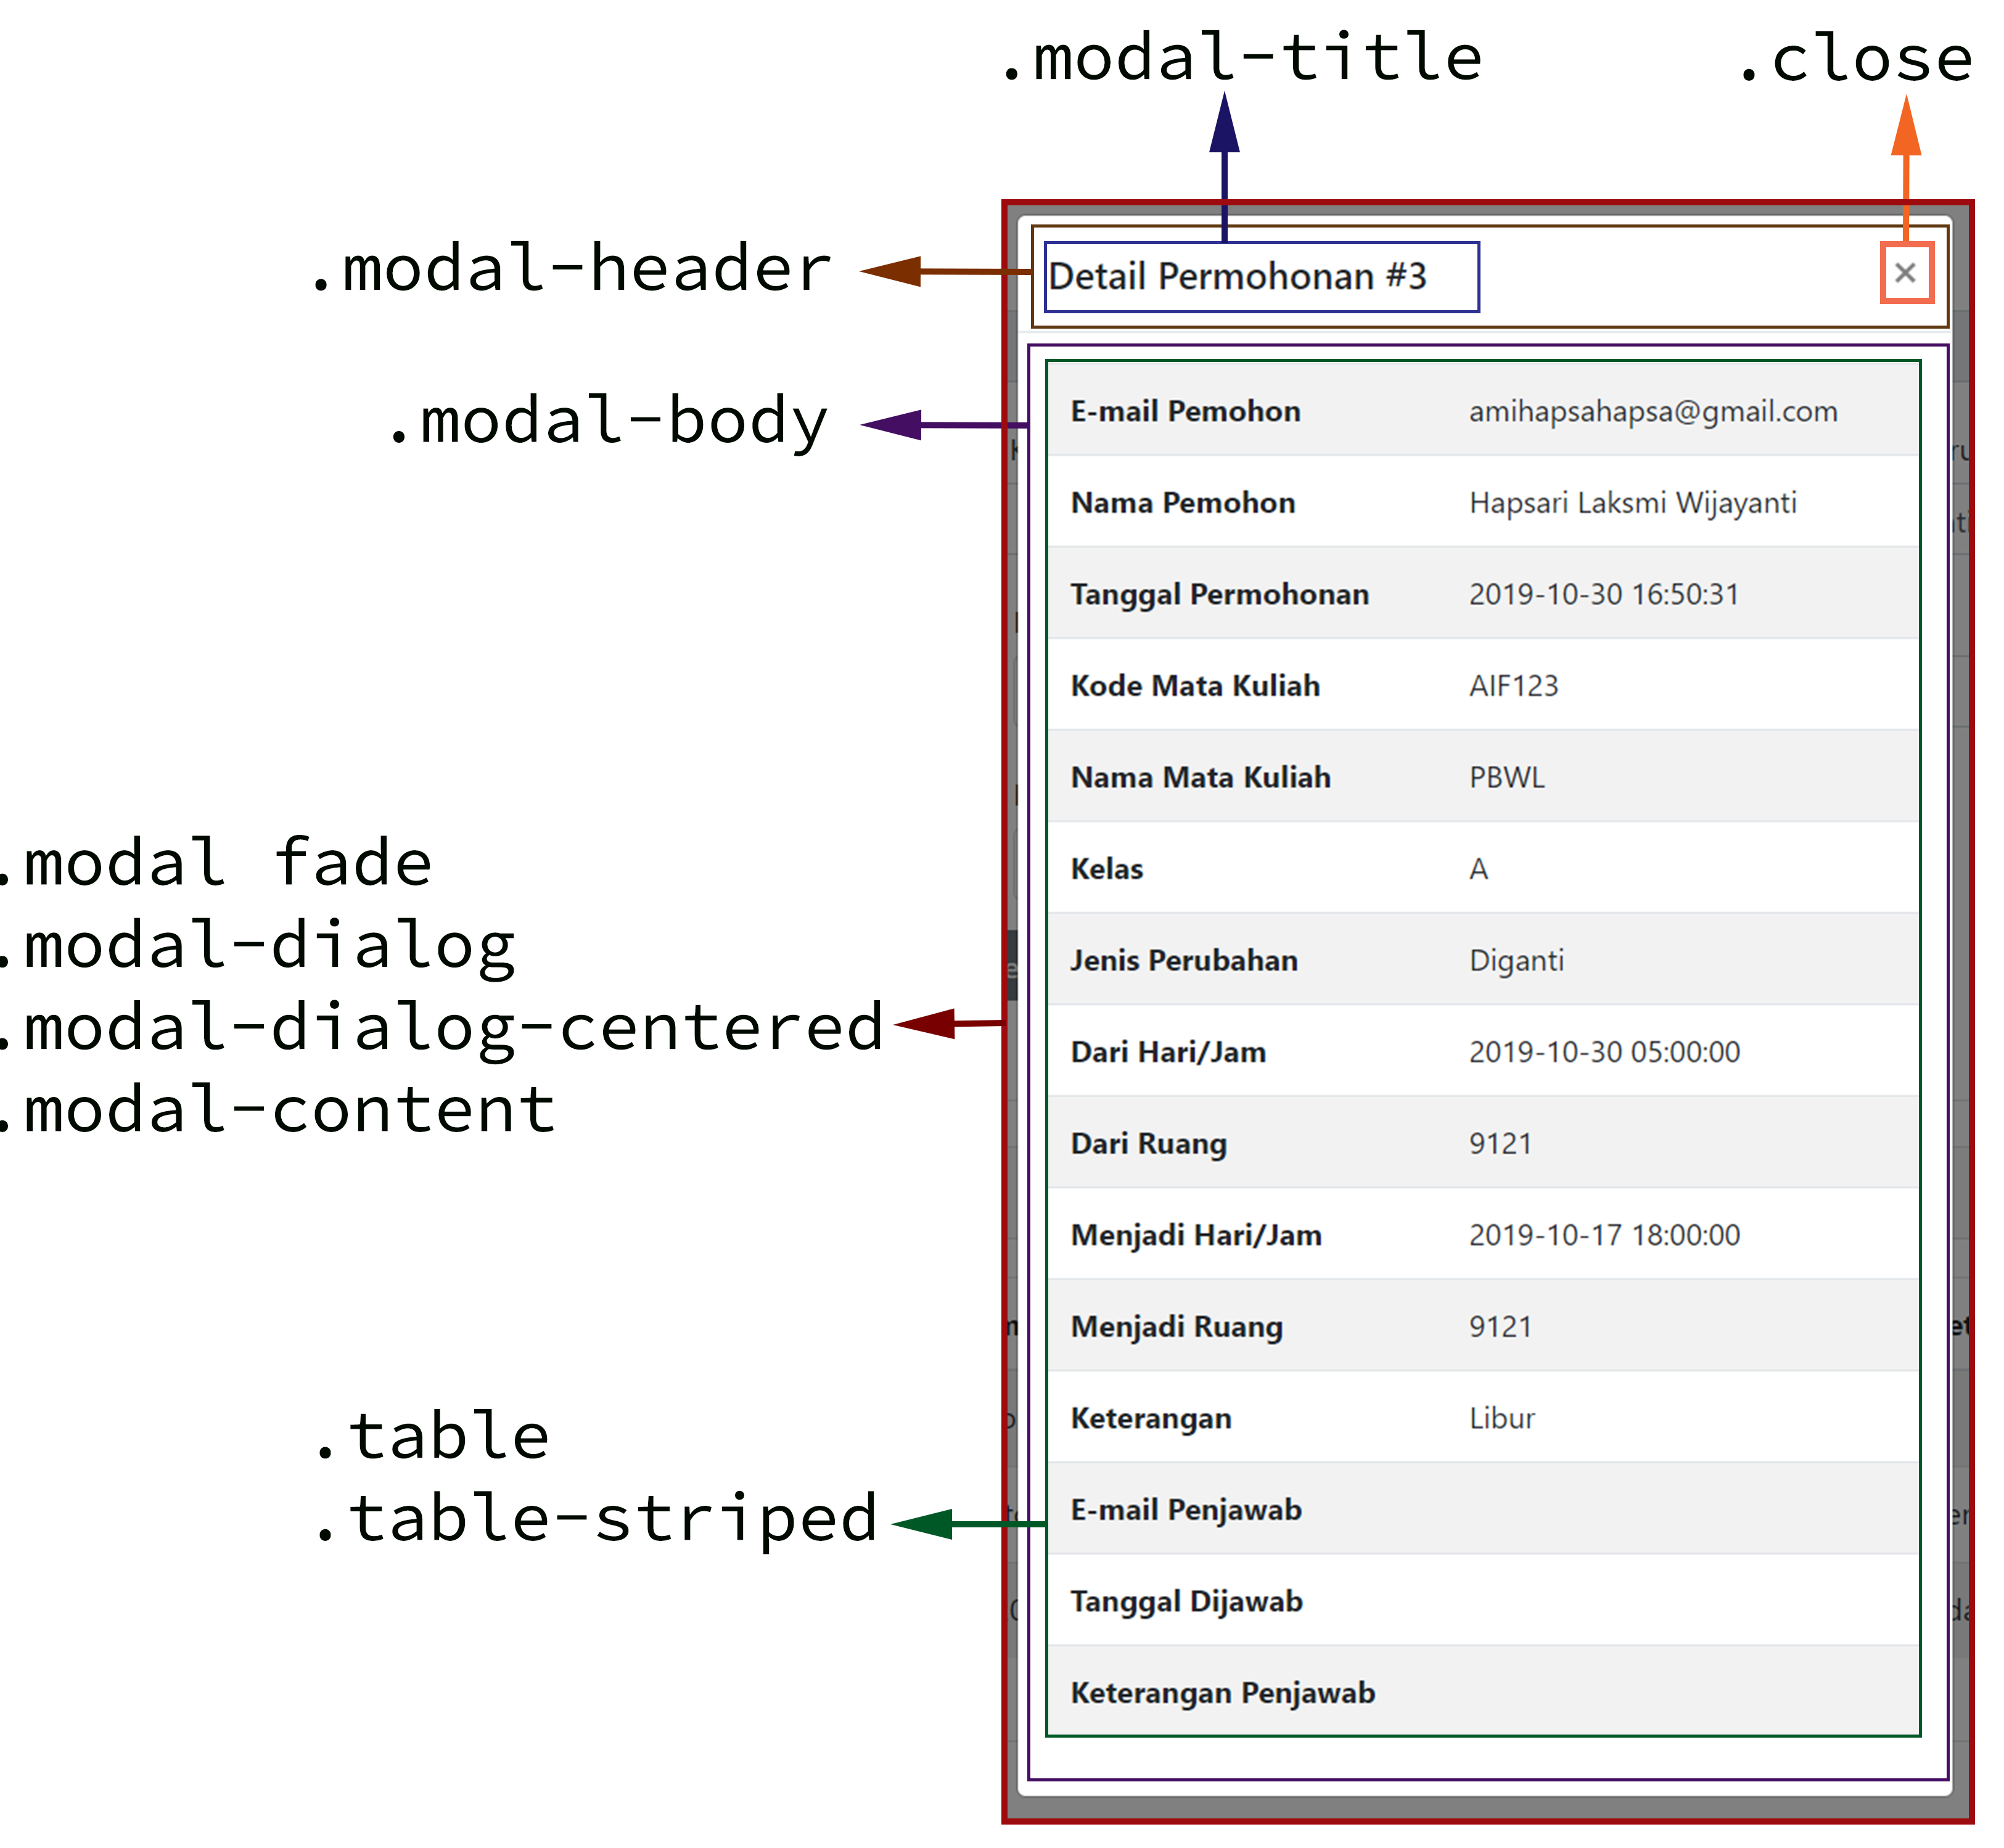
\includegraphics[width=\textwidth,height=\textheight,keepaspectratio]{bootstrap/konversi_modal_lihat_manajemen_perubahan_kuliah.png}
		\caption{Modal lihat.}
	\end{subfigure}	
	\begin{subfigure}[b]{0.45\linewidth} 
		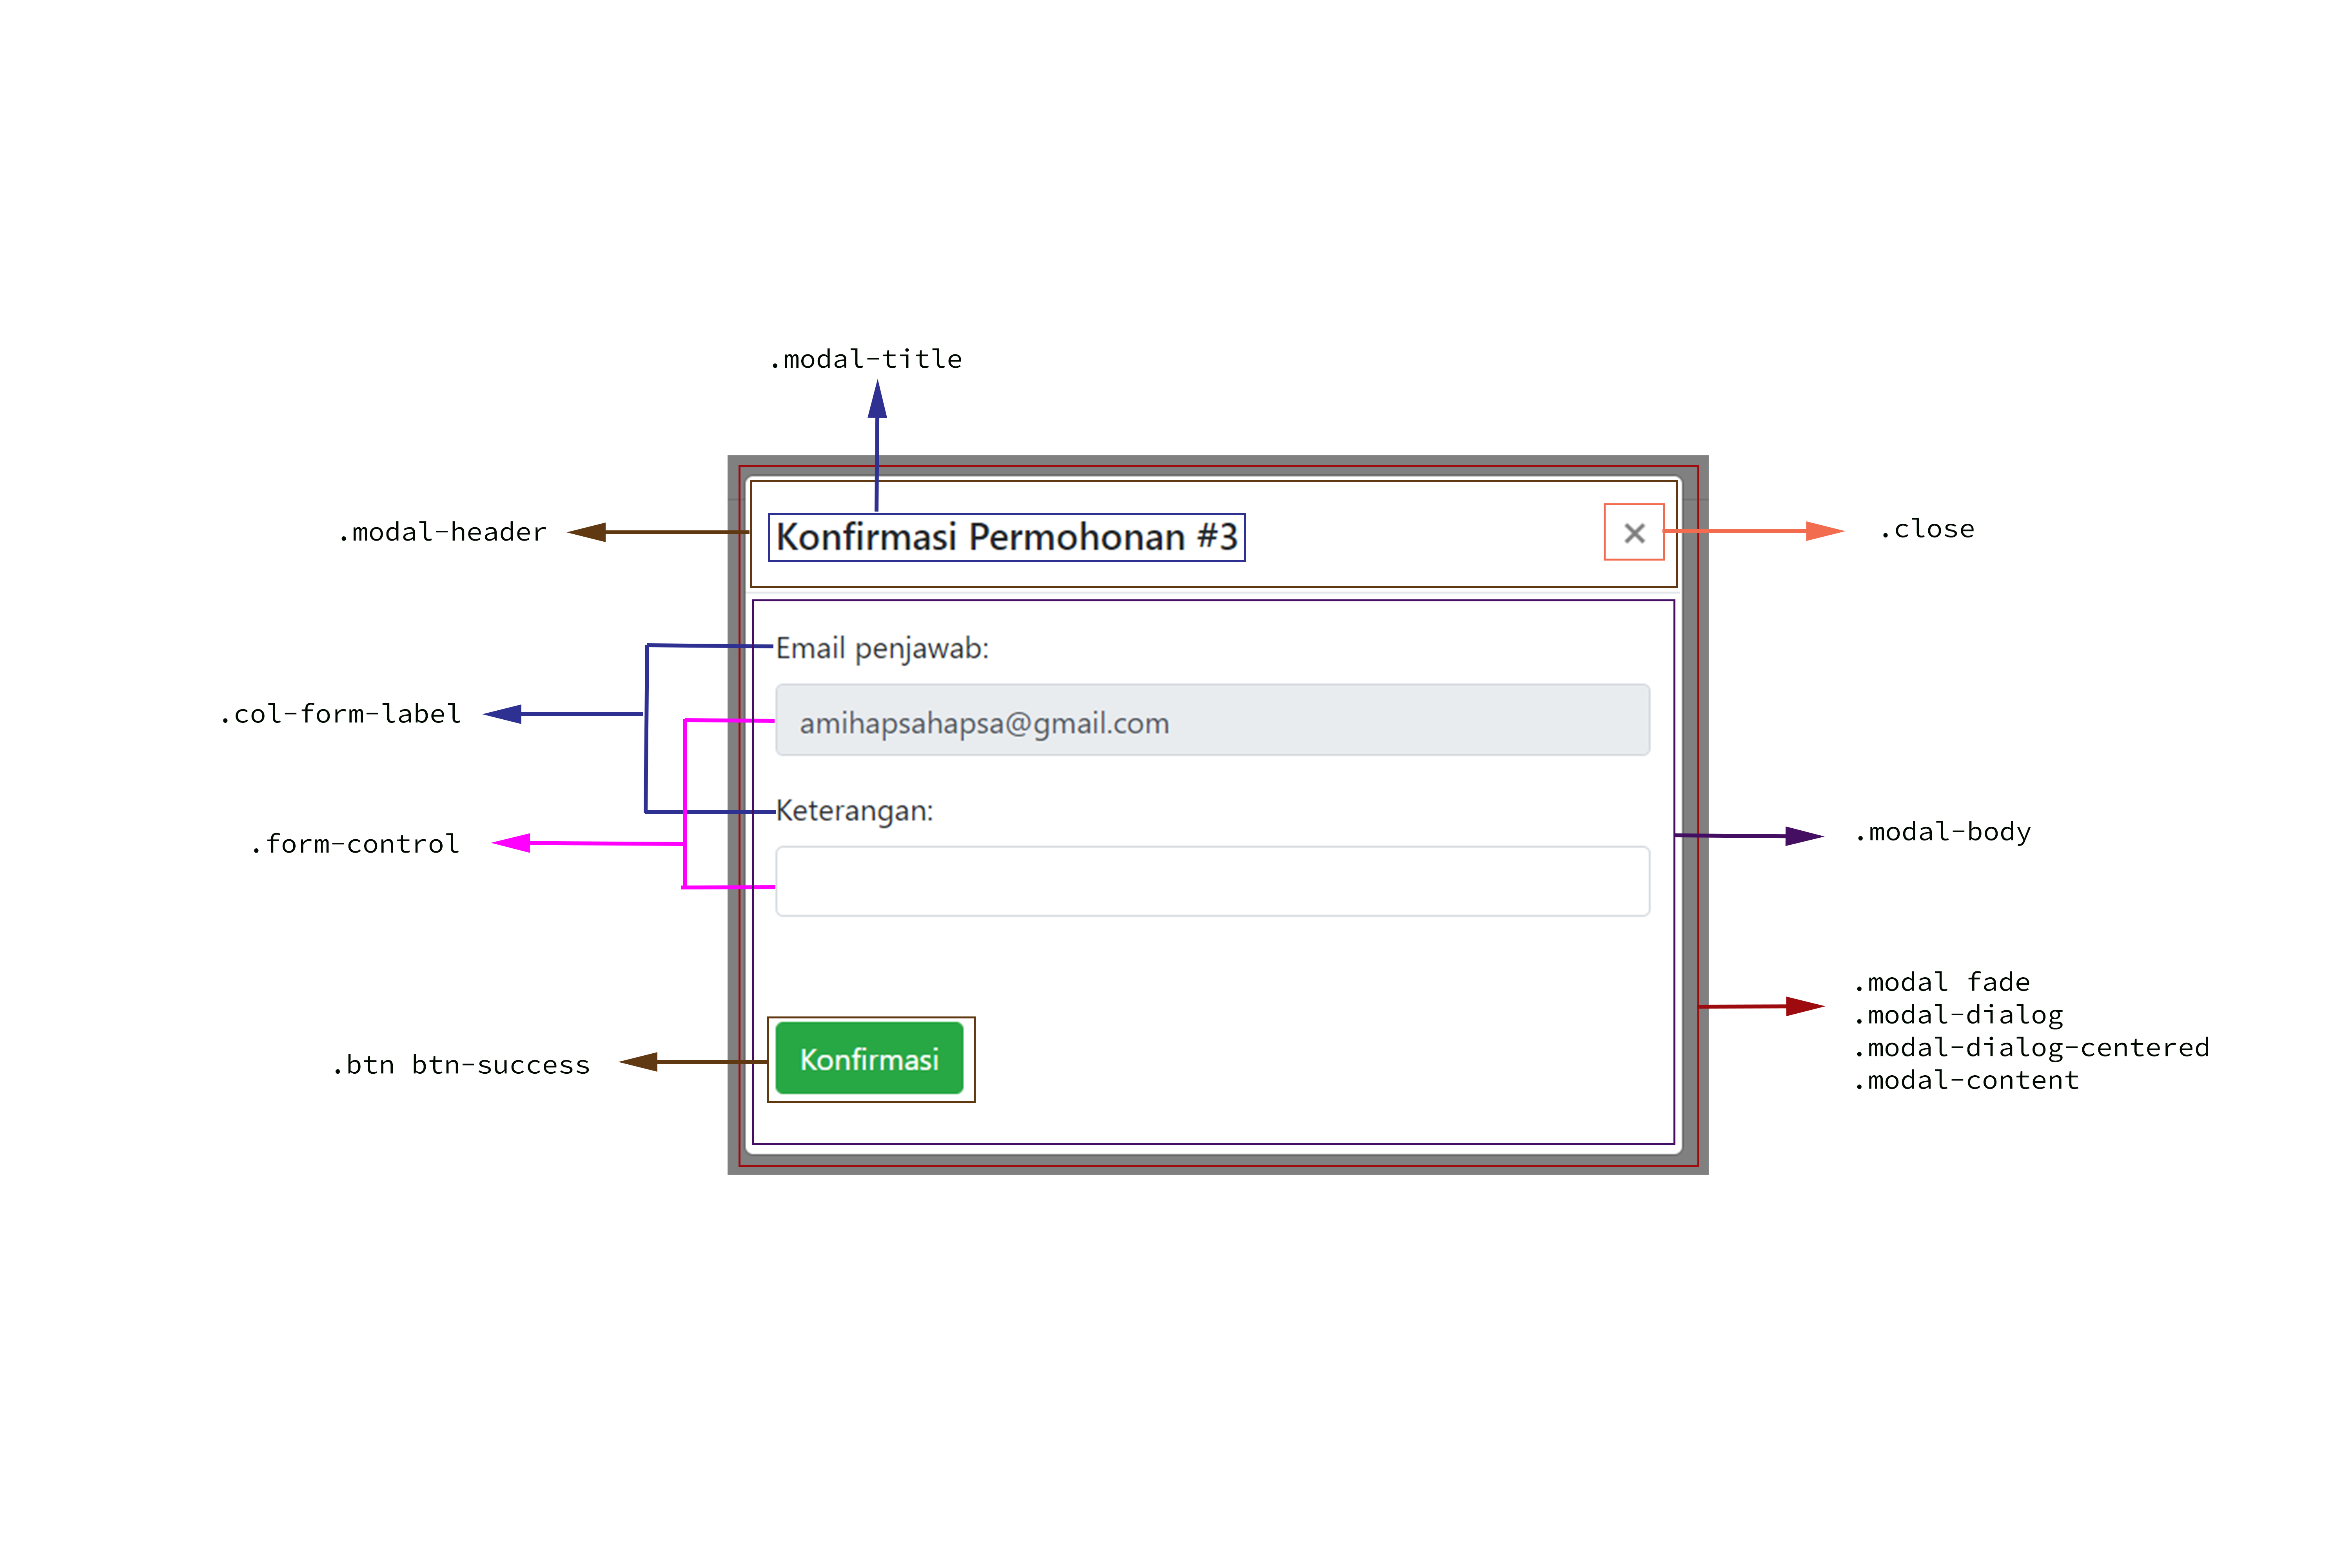
\includegraphics[width=\textwidth,height=\textheight,keepaspectratio]{bootstrap/konversi_modal_like_manajemen_perubahan_kuliah.png}
		\caption{Modal setuju.}
	\end{subfigure}
\end{figure}
\begin{figure}[H]	
	\centering
	\ContinuedFloat
	\begin{subfigure}[b]{0.45\linewidth}  
		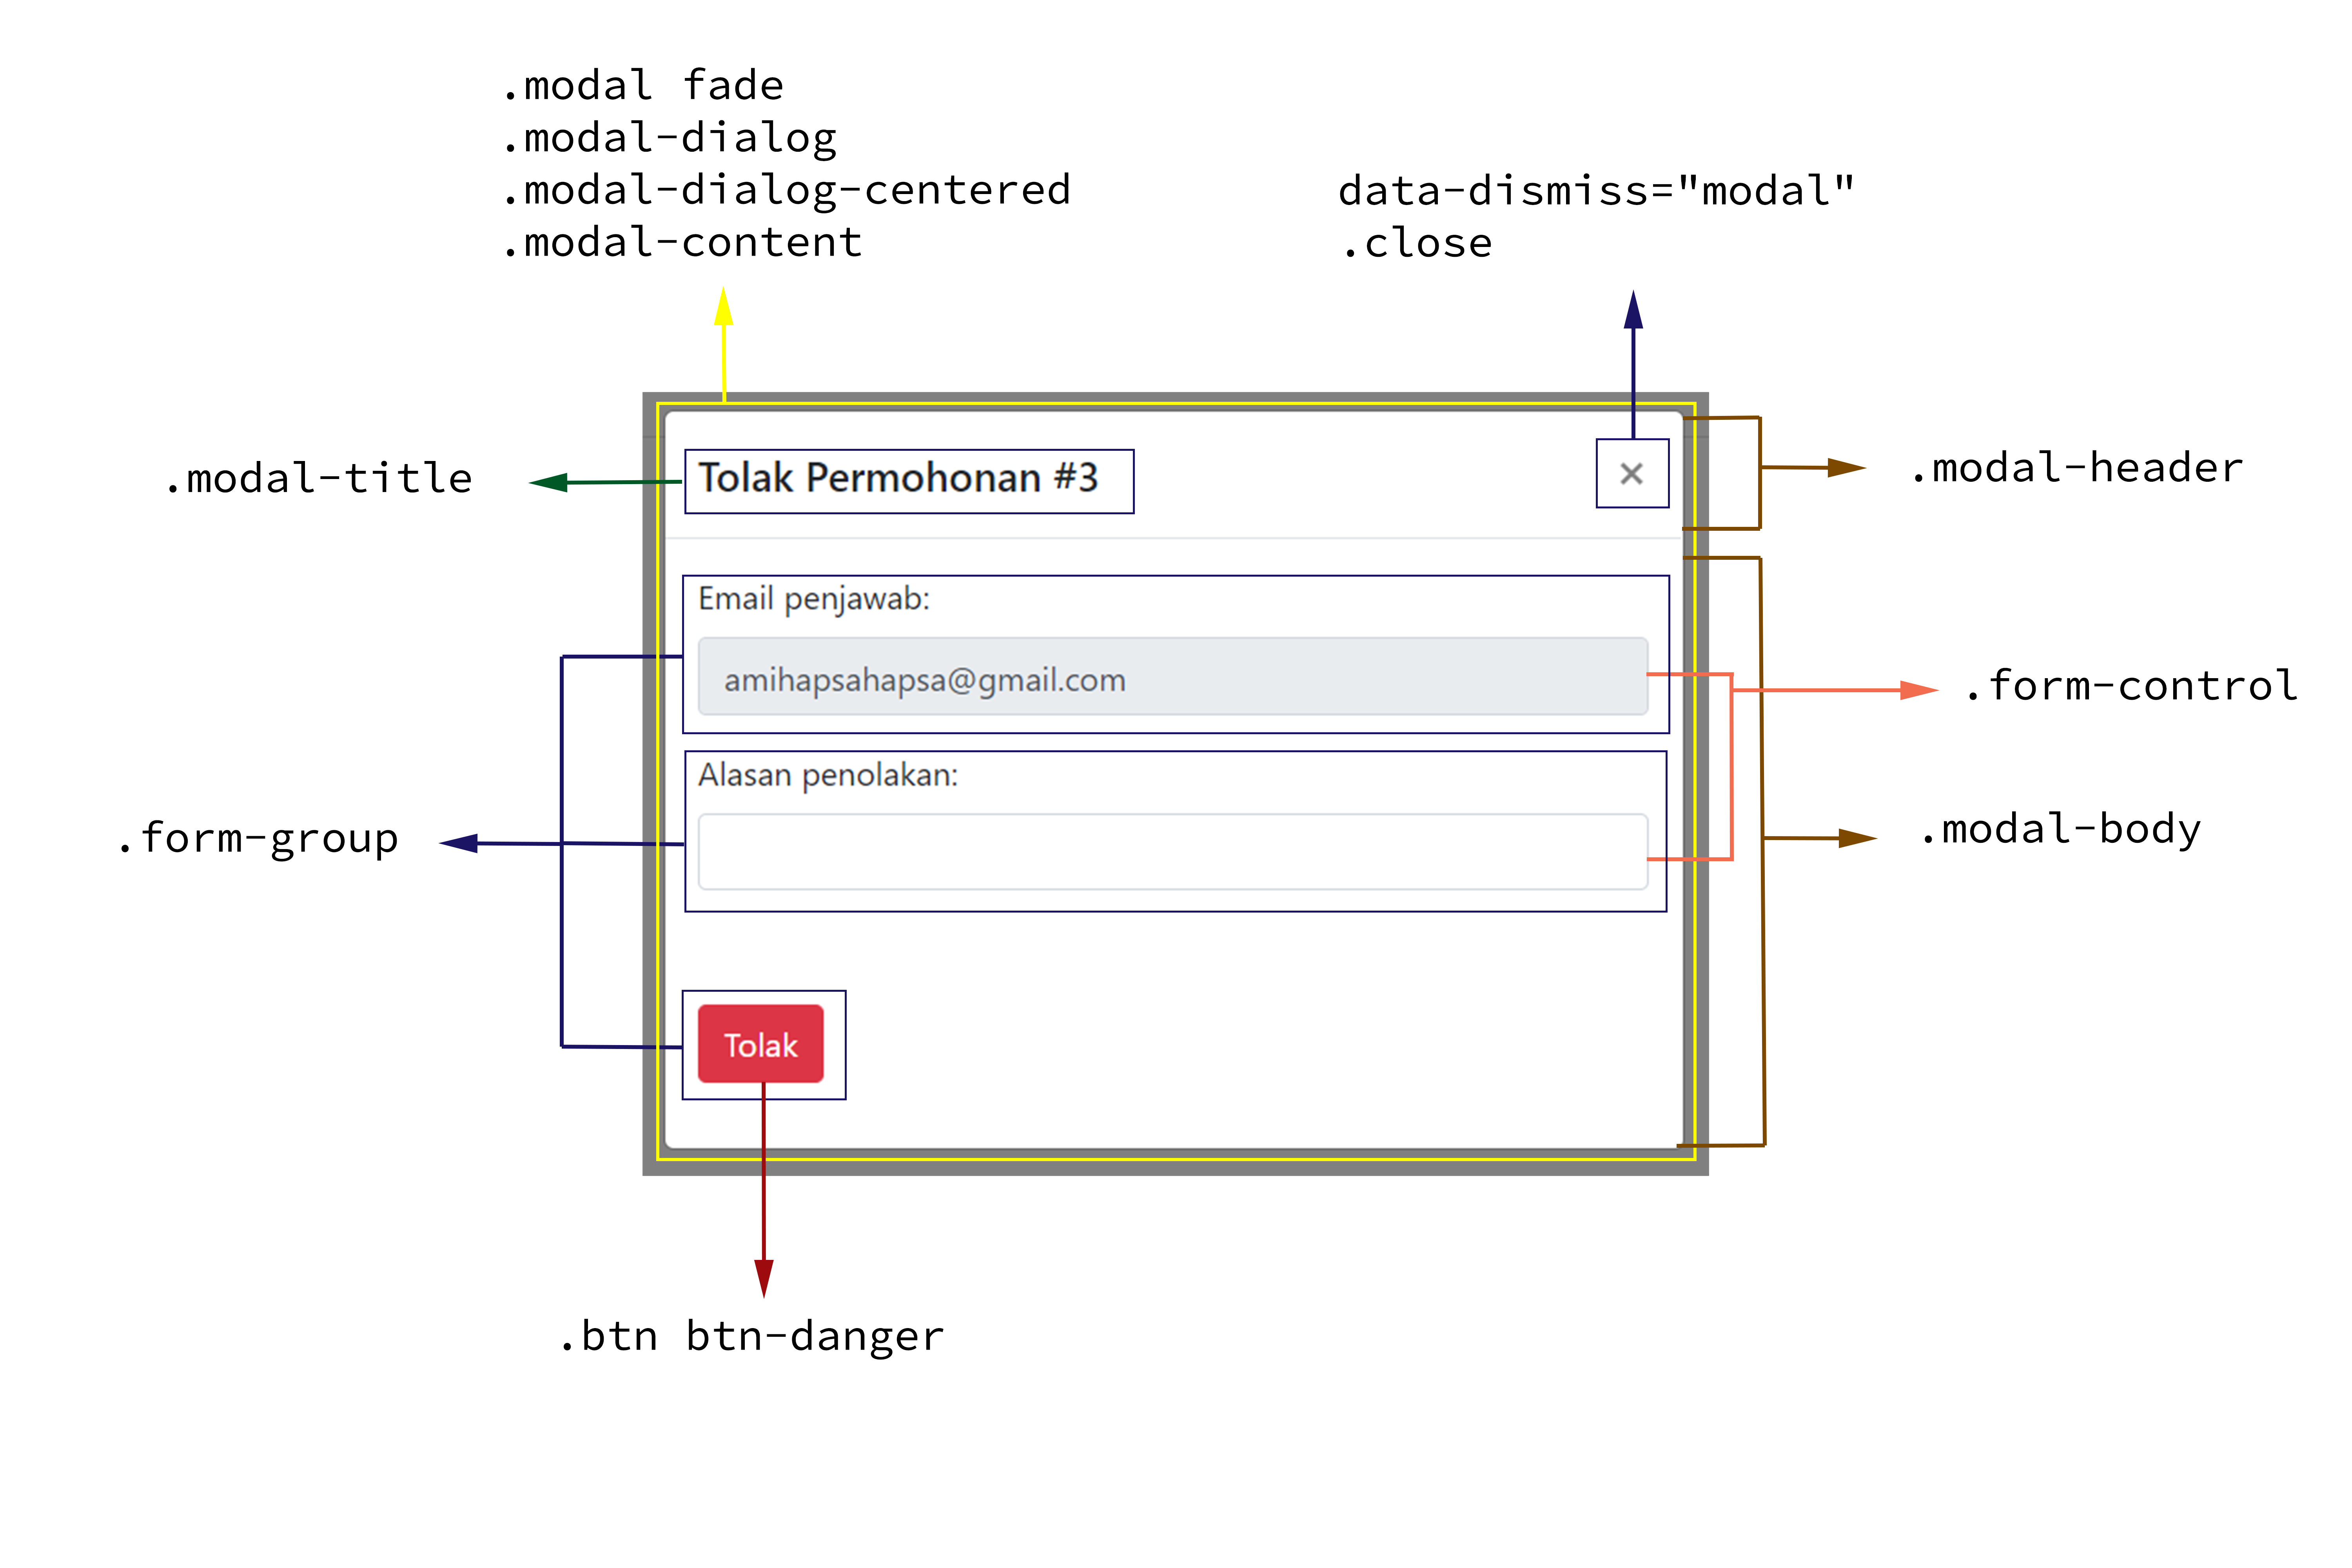
\includegraphics[width=\textwidth,height=\textheight,keepaspectratio]{bootstrap/konversi_modal_dislike_manajemen_perubahan_kuliah.png}
		\caption{Modal tolak.}
	\end{subfigure}
\end{figure}

\begin{figure}[H] 
	\centering
	\ContinuedFloat
	\begin{subfigure}[b]{0.45\linewidth}  
		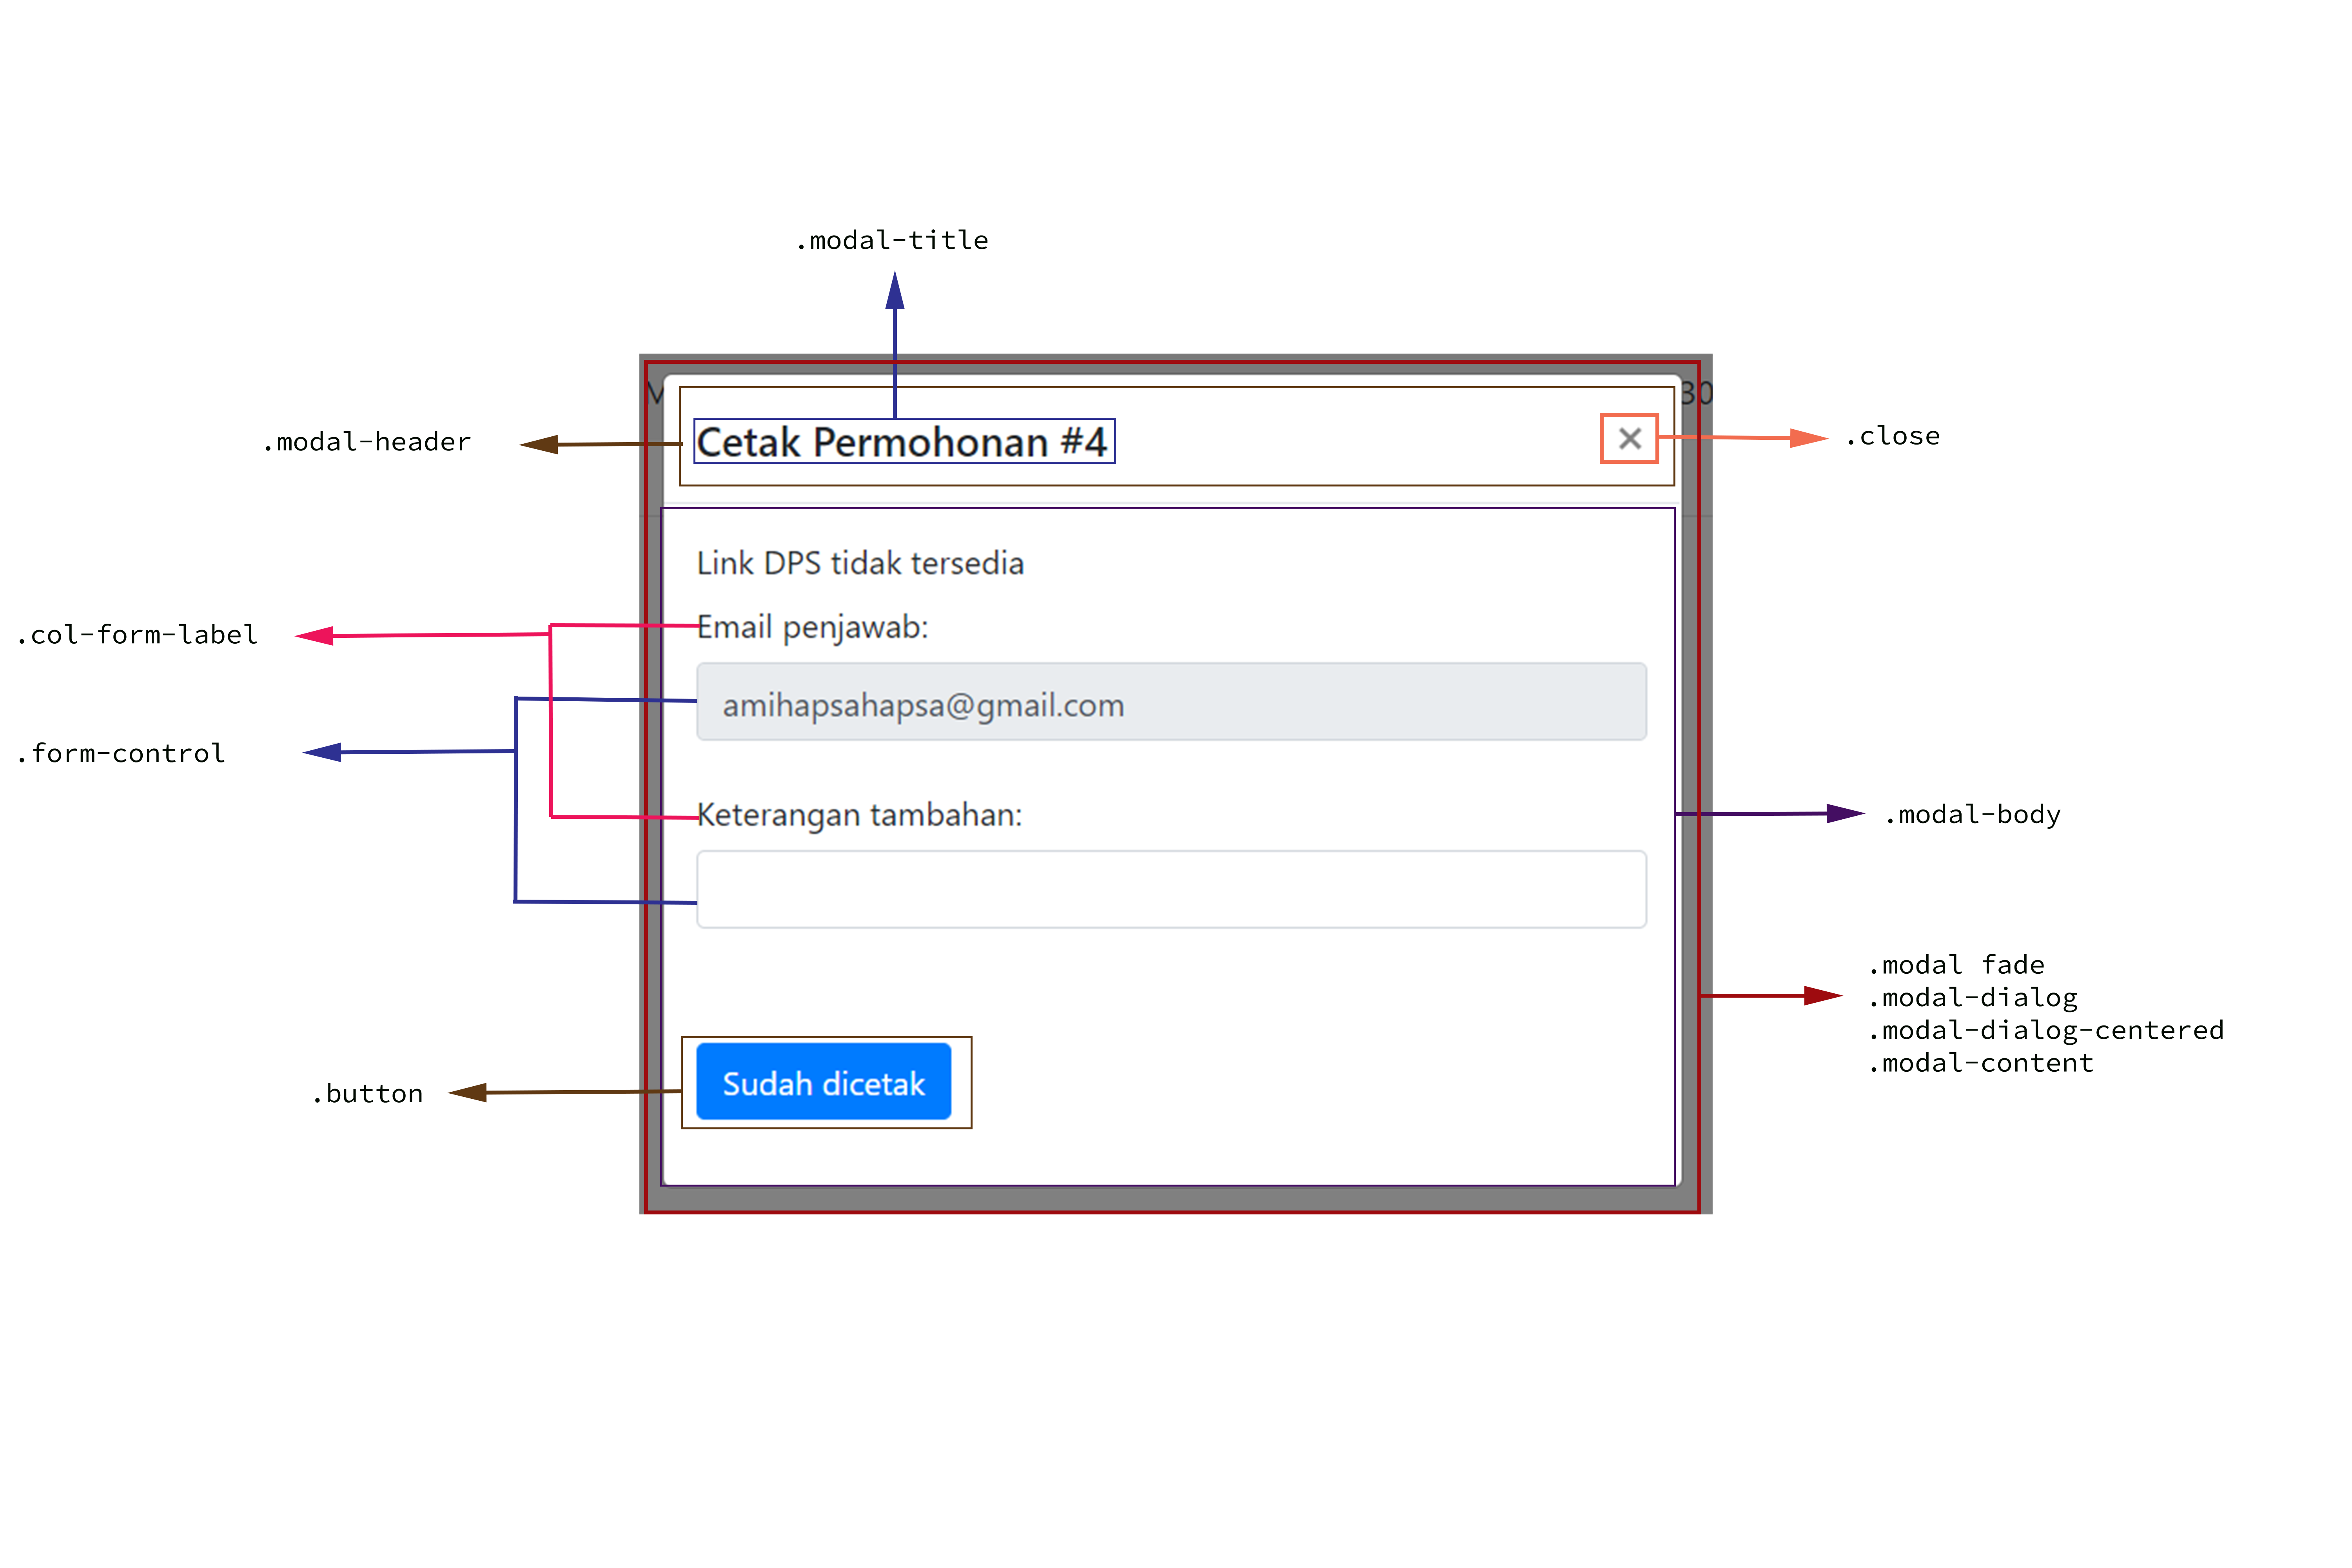
\includegraphics[width=\textwidth,height=\textheight,keepaspectratio]{bootstrap/konversi_modal_print_manajemen_cetak_transkrip.png}
		\caption{Modal print}
	\end{subfigure}	
	\begin{subfigure}[b]{0.45\linewidth}   
		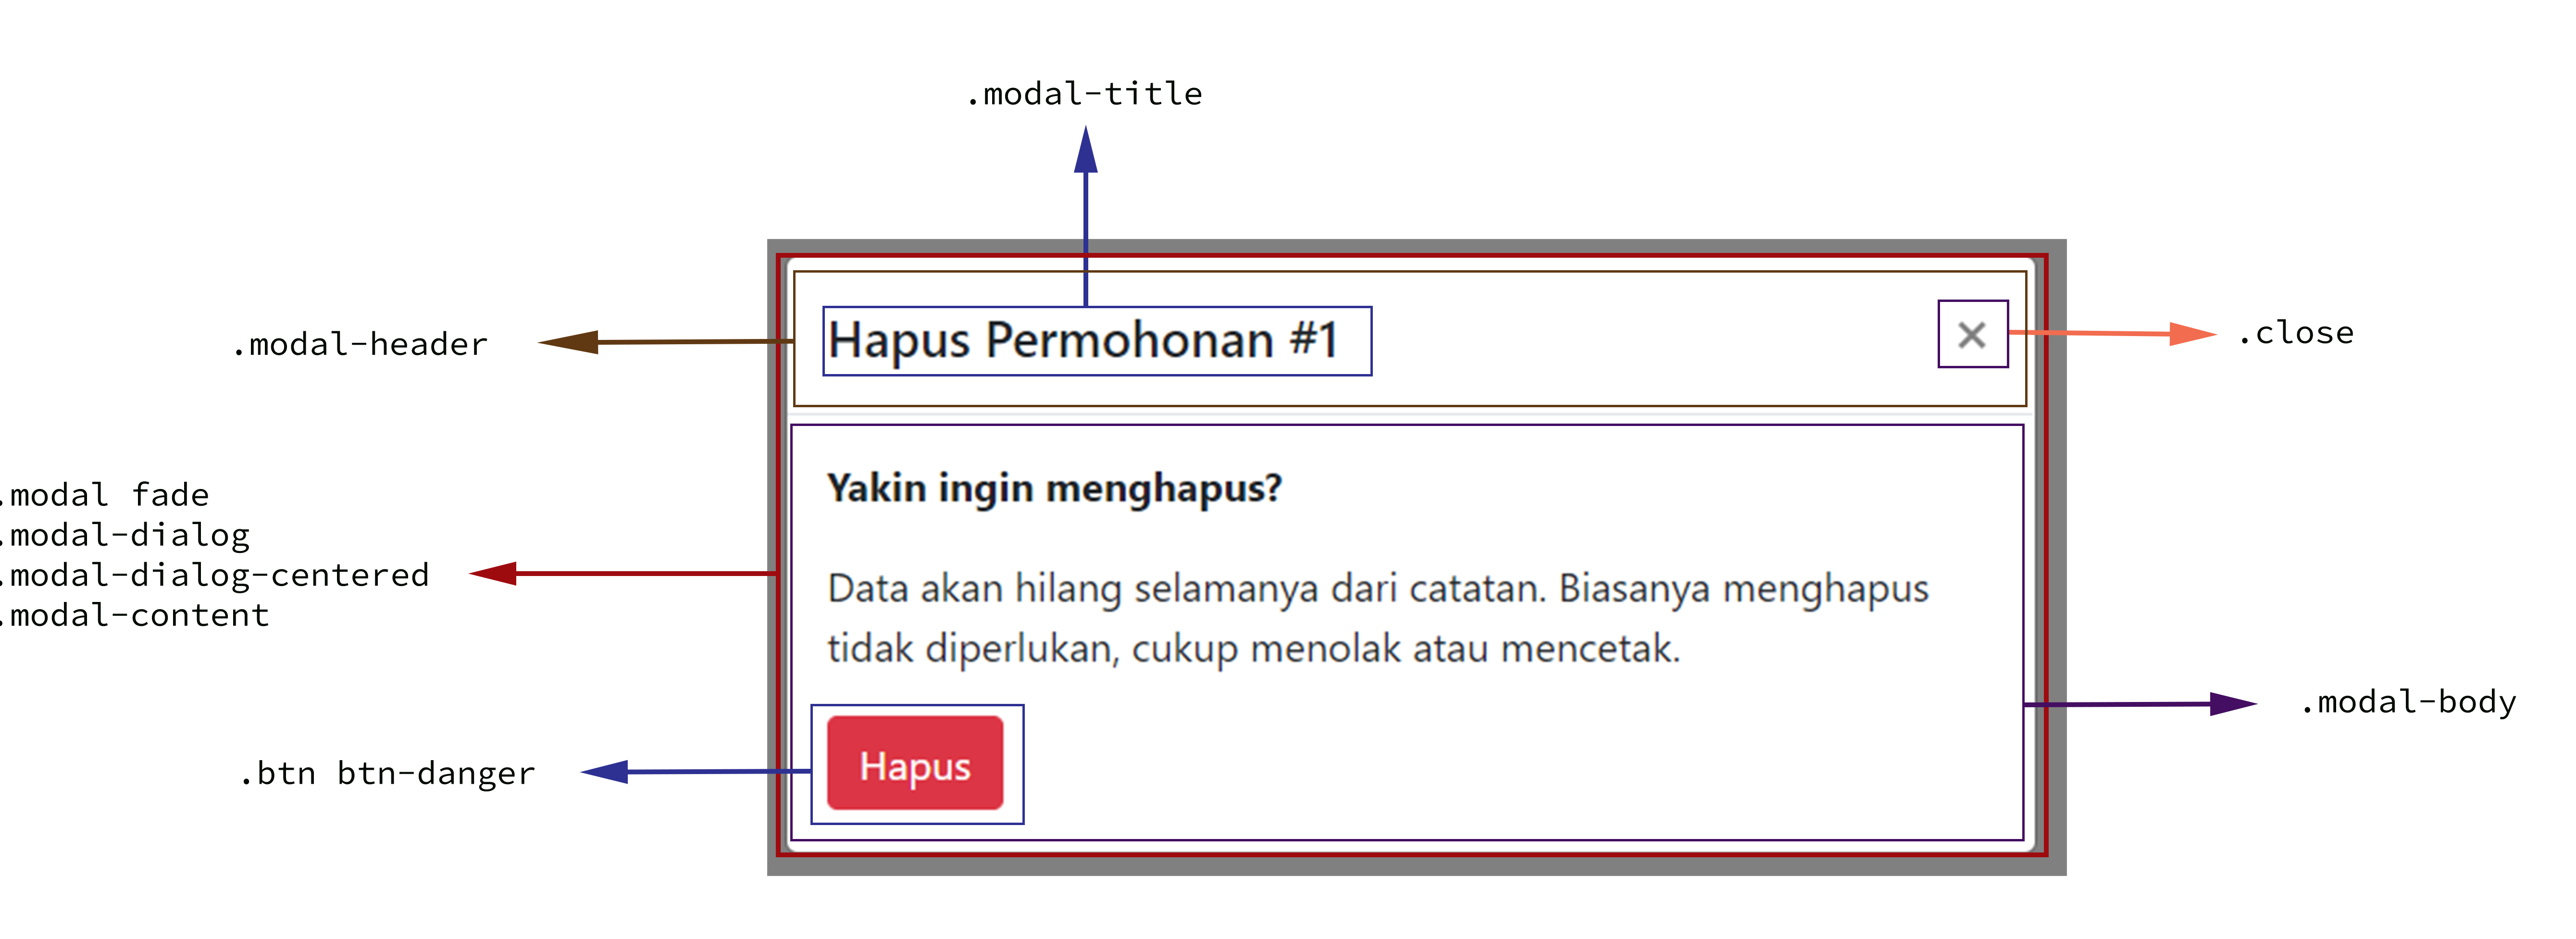
\includegraphics[width=\textwidth,height=\textheight,keepaspectratio]{bootstrap/konversi_modal_trash_manajemen_perubahan_kuliah.png}
		\caption{Modal hapus.}
	\end{subfigure}
	\caption{Konversi modal pada halaman manajemen perubahan kuliah.}
	\label{fig:konversiModalManajemenPerubahanKuliah}
\end{figure}

\begin{lstlisting}[language=diff, caption=Perubahan file \path{\views\PerubahanKuliahManage\main.php},  basicstyle=\ttfamily, frame=single,
columns=fullflexible, keepspaces=true, breaklines=true, label={lst:mainPerubahanKuliahManage}]
diff -r a\www\application\views\PerubahanKuliahManage\main.php b\www\application\views\PerubahanKuliahManage\main.php

57,60c61,71
< 
< <div class="reveal" id="detail<?= $request->id ?>" data-reveal>
<    <h5>Detail Permohonan #<?= $request->id ?></h5>
<      <table class="stack">
---
> <div class="modal fade" id="detail<?= $request->id ?>" tabindex="-1" role="dialog" aria-hidden="true">
> <div class="modal-dialog modal-dialog-centered" role="document">
>     <div class="modal-content">
>         <div class="modal-header">
>             <h5 class="modal-title" id="exampleModalLongTitle">Detail Permohonan #<?= $request->id ?></h5>
>             <button type="button" class="close" data-dismiss="modal" aria-label="Close">
>                 <span aria-hidden="true">&times;</span>
>             </button>
>         </div>
>         <div class="modal-body">
>             <table class="table table-striped">

117c125
< $($menuName).foundation('open');
---
> $($menuName).modal();
\end{lstlisting}

\noindent Catatan untuk kode ~\ref{lst:mainTranskripRequest} dijabarkan dalam tabel ~\ref{table:kodePermintaanCetakTranskrip}:
\begin{table}[H]
	\centering
	\caption{Penjelasan kode permintaan cetak transkrip.}
	\begin{tabularx}{\textwidth}{llX}
		\toprule
		No Line & Implementasi     & Penjelasan\\
		\midrule
		5, 9-13 & \textbf{Modal} & Untuk modal pada Foundation 6 hanya menggunakan satu kelas yaitu \texttt{.reveal} sedangkan pada Bootstrap 4 menggunakan beberapa kelas \texttt{.modal} yang terdiri dari \texttt{.modal-fade, modal-content, modal-header}.\\
		22, 24 & \textbf{kode jQuery modal}  & Memanggil jQuery saat jadwal yang terisi dipilih user.\\		
		\bottomrule
	\end{tabularx}%
	\label{table:modal}
\end{table}




\section{Pengujian}
Bagian pengujian akan menjelaskan dua bagian: skenario pengujian dan hasil pengujian. Pengujian ini akan dijalankan pada server lokal dengan aplikasi XAMPP dan browser web Chrome untuk melihat hasil desain serta menguji fitur yang ada dalam website BlueTape. Pengujian bertujuan memastikan tampilan sudah sesuai dengan tampilan sebelumnya dan semua fitur berjalan dengan baik.
\subsection{Skenario Pengujian}
Skenario pengujian berisi alur yang dilakukan penguji untuk memeriksa setiap fitur dan tampilan dari website. 
\subsubsection{Tampilan Login}
Skenario yang dilakukan penguji untuk \textit{login} pada website BlueTape sebagai berikut:
\begin{enumerate}
	\item \textit{User} mengakses \url{127.0.0.1} pada komputer lokal.
	\item \textit{User} memeriksa link "Petunjuk Penggunaan".
	\item \textit{User} memeriksa tombol "Login dengan Google".
	\item \textit{User} melakukan proses login dengan email admin.
	\item \textit{User} memeriksa notifikasi user pada proses \textit{login} dan \textit{logout}.	
\end{enumerate}

\subsubsection{Menu Navigasi}
Skenario yang dilakukan penguji pada bagian menu navigasi pada website BlueTape sebagai berikut:
\begin{enumerate}
	\item \textit{User} memeriksa letak logo BlueTape dan submenu pada layar \textit{large devices} .
	\item \textit{User} memeriksa letak logo BlueTape dan submenu pada layar \textit{medium} dan \textit{small devices}.	
	\item \textit{User} memeriksa tampilan submenu.
\end{enumerate}

\subsubsection{Konten Permohonan Baru pada Halaman Cetak Transkrip}
Skenario yang dilakukan penguji untuk membuat permohonan baru pada halaman cetak transkrip sebagai berikut:
\begin{enumerate}
	\item Mahasiswa memeriksa \textit{container} dari konten "Permohonan Baru".
	\item Mahasiswa memeriksa label dan input.
	\item Mahasiswa memeriksa tombol "Kirim Permohonan".	
	\item Mahasiswa memeriksa notifikasi \textit{user}.
\end{enumerate}

\subsubsection{Konten Histori Permohonan pada Halaman Cetak Transkrip}
Skenario yang dilakukan penguji untuk melihat histori permohonan pada halaman cetak transkrip sebagai berikut:
\begin{enumerate}
	\item Mahasiswa memeriksa \textit{container} dari konten "Histori Permohonan".
	\item Mahasiswa memeriksa \textit{styling} dari tabel.	
	\item Mahasiswa memeriksa data yang dikirim dari \textit{form} permohonan baru.
	\item Mahasiswa memeriksa penggunaan label berwarna pada kolom "Status".		
	\item Mahasiswa memeriksa penggunaan ikon pada kolom "Aksi".	
\end{enumerate}

\subsubsection{Popup Pesan Detail Permohonan pada Halaman Cetak Transkrip}
Skenario yang dilakukan penguji untuk melihat detail permohonan untuk aksi "Lihat" sebagai berikut:
\begin{enumerate}
	\item Mahasiswa memeriksa penggunaan \textit{popup} untuk menampilkan detail permohonan.
	\item Mahasiswa memeriksa desain pada tabel.
	\item Mahasiswa memeriksa data pada tabel.
\end{enumerate}

\subsubsection{Fitur Pencarian NPM pada Halaman Manajemen Cetak Transkrip}
Skenario yang dilakukan penguji untuk \textit{form} pencarian npm pada halaman manajemen cetak transkrip sebagai berikut:
\begin{enumerate}
	\item Staf tata usaha memeriksa \textit{container} dari konten "Permintaan Transkrip".
	\item Staf tata usaha memeriksa \textit{group label} dari "Cari NPM" pada \textit{form}.	
	\item Staf tata usaha memeriksa \textit{group field} pada \textit{form}.	
	\item Staf tata usaha memeriksa \textit{group button} dari "Cari" pada \textit{form}.
\end{enumerate}

\subsubsection{Tabel Daftar Permintaan Transkrip pada Halaman Manajemen Cetak Transkrip}
Skenario yang dilakukan penguji untuk tabel daftar permintaan pada halaman manajemen cetak transkrip sebagai berikut:
\begin{enumerate}
	\item Staf tata usaha memeriksa desain tabel yang digunakan pada konten "Permintaan Transkrip".
	\item Staf tata usaha memeriksa data yang ditampilkan dalam tabel.
	\item Staf tata usaha memeriksa penggunaan \textit{label} pada kolom "Status" pada \textit{form}.
	\item Staf tata usaha memeriksa penggunaan ikon pada kolom "Aksi" pada \textit{form}.
\end{enumerate}

\subsubsection{Popup Pesan Detail Permohonan pada Konten Permintaan Transkrip}
Skenario yang dilakukan penguji untuk melihat detail permohonan untuk aksi "Lihat" sebagai berikut:
\begin{enumerate}
	\item Staf tata usaha memeriksa penggunaan \textit{popup} untuk menampilkan detail permohonan.
	\item Staf tata usaha memeriksa desain tabel.	
	\item Staf tata usaha memeriksa isi dari tabel.
\end{enumerate}

\subsubsection{Popup Pesan Tolak Permohonan pada Konten Permintaan Transkrip}
Skenario yang dilakukan penguji untuk menolak permohonan untuk aksi "Tolak" sebagai berikut:
\begin{enumerate}
	\item Staf tata usaha memeriksa penggunaan \textit{popup} untuk konfirmasi tolak permohonan.
	\item Staf tata usaha memeriksa label dan \textit{input field} pada \textit{form}.
	\item Staf tata usaha memeriksa tombol "Tolak" pada \textit{form}.	
\end{enumerate}

\subsubsection{Popup Pesan Cetak Permohonan pada Konten Permintaan Transkrip}
Skenario yang dilakukan penguji untuk menolak permohonan untuk aksi "Cetak" sebagai berikut:
\begin{enumerate}
	\item Staf tata usaha memeriksa penggunaan \textit{popup} untuk konfirmasi cetak permohonan.
	\item Staf tata usaha memeriksa label dan \textit{input field} pada \textit{form}.
	\item Staf tata usaha memeriksa tombol "Sudah dicetak" pada \textit{form}.	
\end{enumerate}

\subsubsection{Popup Pesan Hapus Permohonan pada Konten Permintaan Transkrip}
Skenario yang dilakukan penguji untuk menolak permohonan untuk aksi "Hapus" sebagai berikut:
\begin{enumerate}
	\item Staf tata usaha memeriksa penggunaan \textit{popup} untuk konfirmasi hapus permohonan.
	\item Staf tata usaha memeriksa tombol "Hapus" pada \textit{form}.	
\end{enumerate}

\subsubsection{Konten Permohonan Baru pada Halaman Perubahan Kuliah}
Skenario yang dilakukan penguji untuk konten permohonan baru pada halaman perubahan kuliah sebagai berikut:
\begin{enumerate}
	\item Dosen memeriksa \textit{container} dari konten "Permohonan Baru".
	\item Dosen memeriksa penggunaan plugin \textit{DateTimePicker}.
	\item Dosen memeriksa \textit{input field} dan label pada \textit{form}.
	\item Dosen memeriksa tombol "Kirim Permohonan".	
	\item Dosen memeriksa tombol "Tambah Pertemuan Ekstra".
	\item Dosen memeriksa adanya notifikasi \textit{user} ketika melakukan kirim permohonan perubahan kuliah.
\end{enumerate}

\subsubsection{Konten Histori Permohonan pada Halaman Perubahan Kuliah}
Skenario yang dilakukan penguji untuk konten histori permohonan pada halaman perubahan kuliah sebagai berikut:
\begin{enumerate}
	\item Dosen memeriksa \textit{container} dari konten "Histori Permohonan".
	\item Dosen memeriksa \textit{styling} dari tabel.	
	\item Dosen memeriksa data pada kolom "ID" memiliki format teks \textit{bold}.
	\item Dosen memeriksa penggunaan label berwarna pada kolom "Status".			
	\item Dosen memeriksa penggunaan ikon pada kolom "Aksi".
\end{enumerate}

\subsubsection{Popup Pesan Detail Permohonan pada Konten Histori Permohonan}
Skenario yang dilakukan penguji untuk melihat detail permohonan untuk aksi "Lihat" sebagai berikut:
\begin{enumerate}
	\item Dosen memeriksa penggunaan \textit{popup} untuk menampilkan detail permohonan.
	\item Dosen memeriksa penggunaan tabel.	
\end{enumerate}

\subsubsection{Konten Permohonan Perubahan Kuliah pada Halaman Manajemen Perubahan Kuliah}
Skenario yang dilakukan penguji untuk konten permohonan perubahan kuliah pada halaman permohonan perubahan kuliah sebagai berikut:
\begin{enumerate}
	\item Staf tata usaha memeriksa \textit{container} dari konten "Permohonan Perubahan Kuliah".
	\item Staf tata usaha memeriksa \textit{styling} dari tabel.	
	\item Staf tata usaha memeriksa data pada kolom "ID" memiliki format teks \textit{bold}.
	\item Staf tata usaha memeriksa penggunaan label berwarna pada kolom "Status".			
	\item Staf tata usaha memeriksa penggunaan ikon pada kolom "Aksi".
\end{enumerate}

\subsubsection{Popup Pesan Detail Permohonan pada Konten Permohonan Perubahan Kuliah}
Skenario yang dilakukan penguji untuk melihat detail permohonan untuk aksi "Lihat" sebagai berikut:
\begin{enumerate}
	\item Staf tata usaha memeriksa penggunaan \textit{popup} untuk menampilkan detail permohonan.	
	\item Staf tata usaha memeriksa penggunaan tabel.	
\end{enumerate}

\subsubsection{Popup Pesan Konfirmasi Permohonan pada Konten Permohonan Perubahan Kuliah}
Skenario yang dilakukan penguji untuk konfirmasi permohonan untuk aksi "Konfirmasi" sebagai berikut:
\begin{enumerate}
	\item Staf tata usaha memeriksa penggunaan \textit{popup} untuk konfirmasi permohonan.
	\item Staf tata usaha memeriksa label dan \textit{input field} pada \textit{form}.
	\item Staf tata usaha memeriksa tombol "Konfirmasi" pada \textit{form}.	
\end{enumerate}

\subsubsection{Popup Pesan Tolak Permohonan pada Konten Permohonan Perubahan Kuliah}
Skenario yang dilakukan penguji untuk modal tolak permohonan untuk aksi "Tolak" sebagai berikut:
\begin{enumerate}
	\item Staf tata usaha memeriksa penggunaan \textit{popup} untuk konfirmasi tolak permohonan.
	\item Staf tata usaha memeriksa label dan \textit{input field} pada \textit{form}.
	\item Staf tata usaha memeriksa tombol "Tolak" pada \textit{form}.	
\end{enumerate}

\subsubsection{Popup Pesan Hapus Permohonan pada Konten Permohonan Perubahan Kuliah}
Skenario yang dilakukan penguji untuk menolak permohonan untuk aksi "Tolak" sebagai berikut:
\begin{enumerate}
	\item Staf tata usaha memeriksa penggunaan \textit{popup} untuk konfirmasi hapus permohonan.
	\item Staf tata usahamemeriksa label dan \textit{input field} pada \textit{form}.
	\item Staf tata usaha memeriksa tombol "Hapus" pada \textit{form}.	
\end{enumerate}

\subsubsection{Konten Tambah Jadwal pada Halaman Entri Jadwal Dosen}
Skenario yang dilakukan penguji pada konten tambah jadwal dosen di halaman entri jadwal dosen sebagai berikut:
\begin{enumerate}
	\item Dosen memeriksa \textit{container} dari konten "Tambah Jadwal".	
	\item Dosen memeriksa label pada \textit{form}. 
	\item Dosen memeriksa \textit{input field} pada \textit{form}.
	\item Dosen memeriksa \textit{plugin} yang digunakan pada \textit{form field} "Jam Mulai".
	\item Dosen memeriksa tombol "Tambah".
\end{enumerate}

\subsubsection{Konten Daftar Jadwal pada Halaman Entri Jadwal Dosen}
Skenario yang dilakukan penguji pada konten daftar jadwal di halaman entri jadwal dosen sebagai berikut:
\begin{enumerate}
	\item Dosen memeriksa \textit{container} dari konten "Daftar Jadwal".
	\item Dosen memeriksa \textit{styling} dari tabel.	
	\item Dosen memeriksa \textit{stylig} untuk \textit{cell} yang memiliki nama jadwal.			
	\item Dosen memeriksa tombol "Delete All".
	\item Dosen memeriksa tombol "Ekspor ke XLS".
\end{enumerate}

\subsubsection{Popup Pesan Edit Jadwal pada Konten Daftar Jadwal}
Skenario yang dilakukan penguji pada modal edit jadwal sebagai berikut:
\begin{enumerate}
	\item Dosen memeriksa penggunaan \textit{popup} untuk melakukan edit jadwal.
	\item Dosen memeriksa label dan \textit{input field} pada \textit{form}. 
	\item Dosen memeriksa tombol "Save" pada \textit{form}.
	\item Dosen memeriksa tombol "Delete" pada \textit{form}.
\end{enumerate}

\subsubsection{Halaman Lihat Jadwal Dosen}
Skenario yang dilakukan penguji pada halaman entri jadwal dosen sebagai berikut:
\begin{enumerate}
	\item Mahasiswa memeriksa \textit{container} dari halaman entri jadwal dosen.
	\item Mahasiswa memeriksa \textit{tabs} untuk setiap jadwal dosen.
	\item Mahasiswa memeriksa \textit{styling} dari tabel.	
	\item Mahasiswa memeriksa \textit{stylig} untuk \textit{cell} yang memiliki nama jadwal.
	\item Mahasiswa memeriksa tombol "Ekspor ke XLS".
\end{enumerate}

\subsection{Hasil Pengujian}
Pada bagian ini akan dijabarkan hasil pengujian dari skenario yang sudah dirancang sebelumnya. Setiap skenario akan diuji berdasarkan tindakan yang sudah dibuat, kemudian akan ditentukan pengujian berhasil atau tidak.
\subsubsection{Login}
Berikut ini hasil pengujian dari halaman login yang terlihat pada tabel ~\ref{hasil:Login}.
\begin{table}[H]
	\centering 
	\caption{Hasil pengujian halaman login.}
	\label{hasil:Login}
	\begin{tabular}{|c|c|p{0.60\textwidth}|}
		\toprule
		\textbf{Langkah} & \textbf{Hasil} & \textbf{Tindakan}\\
		\textbf{Ke} & \textbf{(Sukses / Tidak)} & \\		
		\midrule
		1 & Sukses & Mengakses website menggunakan \url{http://127.0.0.1} pada komputer lokal.\\
		\hline
		2 & Sukses & "Petunjuk Penggunaan" berbentuk link.\\
		\hline
		3 & Sukses & -.\\
		\hline
		4 & Sukses & - \textit{Field} dapat diisi oleh teks.\\									
		\hline
		5 & Sukses & - Melihat notifikasi berwarna biru saat proses \textit{logout} berhasil.\\
		&& - Melihat notifikasi berwarna merah saat mengakses halaman \url{http://127.0.0.1/CetakTranskripRequest} dengan kondisi tidak \textit{login}.\\
		\bottomrule		
	\end{tabular} 
\end{table}

\subsubsection{Menu Navigasi}
Berikut ini hasil pengujian dari menu navigasi yang terlihat pada tabel ~\ref{hasil:MenuNavigasi}.
\begin{table}[H]
	\centering 
	\caption{Hasil pengujian menu navigasi}
	\label{hasil:MenuNavigasi}
	\begin{tabular}{|c| c| p{0.60\textwidth}|}
		\toprule
		\textbf{Langkah Ke} & \textbf{Hasil} & \textbf{Tindakan}\\
		\textbf{Ke} & \textbf{(Sukses / Tidak)} &\\
		\midrule.
		1&Sukses& - Posisi logo BlueTape terletak disebelah kiri. \\
		&& - Posisi submenu keseluruhan halaman website terletak secara horizontal disebelah kiri logo BlueTape. \\
		&& - Posisi submenu "Log Out" berada disebelah kanan menu navigasi. \\
		\hline
		2 & Sukses & - Posisi logo BlueTape terletak disebelah kiri menu navigasi. \\
		&& - Terdapat sebuah ikon menu disebelah kanan menu navigasi. \\
		&& - Submenu berada pada mode \textit{hide} dan dapat ditampilkan setelah \textit{user} memilih ikon menu. \\
		&& - Memeriksa teks setiap sub-menu aktif memiliki warna yang berbeda dengan sub-menu yang tidak aktif. \\		
		\bottomrule		
	\end{tabular} 
\end{table}

\subsubsection{Konten Permohonan Baru pada Halaman Cetak Transkrip}
Berikut ini hasil pengujian dari konten permohonan baru pada halaman cetak transkrip yang terlihat pada tabel ~\ref{hasil:PermohonanBaru}.
\begin{table}[H]
	\centering 
	\caption{Hasil pengujian konten permohonan baru cetak transkrip}
	\label{hasil:PermohonanBaru}
	\begin{tabular}{|c| c| p{0.60\textwidth}|}
		\toprule
		\textbf{Langkah} & \textbf{Hasil} & \textbf{Tindakan}\\
		\textbf{Ke} & \textbf{(Sukses / Tidak)} &\\
		\midrule
		1&Sukses&Konten dikelilingi oleh \textit{border} yang memisahkan antara judul dan isi konten.\\
		\hline
		2&Sukses& - Memeriksa kolom "Yang memohon", "NPM" dan "Nama" memiliki lebar 4 grid dilayar \textit{large} dan 12 grid pada layar \textit{medium} dan \textit{small}.\\		
		&& - Memeriksa kolom "Tipe Transkrip" memiliki lebar 6 grid pada layar \textit{large} dan 12 grid pada layar \textit{medium} dan \textit{small}.\\
		&& - Memeriksa kolom "Keperluan" memiliki lebar 6 grid pada layar \textit{large} dan 12 grid pada layar \textit{medium} dan \textit{small}.\\
		&& - Memeriksa \textit{form field} "Keperluan" menggunakan input \textit{select}.\\
		\hline
		3&Sukses&Memeriksa tombol "Kirim Permohonan" memiliki warna biru.\\
		\hline
		4&Sukses& - Memeriksa adanya notifikasi berwarna merah berisi "Maaf, gagal mengirim email notifikasi.".\\
		&& - Memeriksa adanya notifikasi berwarna biru  berisi "Permintaan cetak transkrip sudah terkirim. Silahkan cek statusnya secara berkala disitus ini.\\		
		\bottomrule		
	\end{tabular} 
\end{table}


\subsubsection{Konten Histori Permohonan pada Halaman Cetak Transkrip}
Berikut ini hasil pengujian dari konten permohonan baru pada halaman cetak transkrip yang terlihat pada tabel ~\ref{hasil:HistoriPermohonan}.
\begin{table}[H]
	\centering 
	\caption{Hasil pengujian konten histori permohonan cetak transkrip}
	\label{hasil:HistoriPermohonan}
	\begin{tabular}{|c| c| p{0.60\textwidth}|}
		\toprule
		\textbf{Langkah Ke} & \textbf{Hasil} & \textbf{Tindakan}\\
		\textbf{Ke} & \textbf{(Sukses / Tidak)} &\\
		\midrule
		1&Sukses&Memeriksa konten dikelilingi oleh \textit{border} yang memisahkan antara judul dan isi konten.\\
		\hline
		2&Sukses&- Memeriksa tabel memiliki kolom bergaris berwarna putih dan abu-abu.\\
		&&- Memeriksa baris judul tabel dan kolom "ID" menampilkan data dengan teks \textit{bold}.\\
		\hline
		3&Sukses& - Memeriksa kolom "ID" berisi nomor dengan format \textit{bold}.\\
		&& - Kolom "Status" berisi sebuah label berisi teks. \\
		&& - Kolom "Tanggal Permohonan" berisi teks yang memiliki format"[nama hari], [tanggal][nama bulan][tahun]" seperti "Senin, 28 Mei 2020" \\
		&& - Kolom "Tipe Transkrip" teks.\\
		\hline
		4&Sukses& - Adanya label "TUNGGU" berwarna abu-abu.\\
		&& - Adanya label "DITOLAK" berwarna merah.\\
		&& - Adanya label "DICETAK" berwarna hijau.\\
		\hline
		5&Sukses& Adanya ikon mata pada kolom "Aksi".\\
		
		\bottomrule		
	\end{tabular} 
\end{table}


\subsubsection{Popup Pesan Detail Permohonan pada Halaman Cetak Transkrip}
Berikut ini hasil pengujian dari popup pesan detail permohonan pada halaman cetak transkrip yang terlihat pada tabel ~\ref{hasil:DetailCetakTranskrip}.
\begin{table}[H]
	\centering 
	\caption{Hasil pengujian detail permohonan cetak transkrip.}
	\label{hasil:DetailCetakTranskrip}
	\begin{tabular}{|c| c| p{0.60\textwidth}|}
		\toprule
		\textbf{Langkah} & \textbf{Hasil} & \textbf{Tindakan}\\
		\textbf{Ke} & \textbf{(Sukses / Tidak)} &\\
		\midrule
		1&Sukses& - Memeriksa popup pesan menampilkan judul "Detail Permohonan [ID]" dan isi pesan menampilkan sebuah tabel.\\
		&& - Memeriksa mode popup dapat ditutup oleh \textit{user}.\\
		\hline
		2&Sukses&- Memeriksa tabel memiliki kolom bergaris berwarna putih dan abu-abu.\\
		&& - Memeriksa data judul kolom ditampilkan dengan teks \textit{bold}.	\\	
		\hline
		3&Sukses&- Kolom "Email Pemohon" berisi teks dengan mode \textit{read-only}.\\
		&&- Kolom "Nama Pemohon" berisi teks dengan mode \textit{read-only}.\\
		&&- Kolom "Tanggal Permohonan" berisi format "[Tahun]-[Bulan]-[Tanggal] [Jam]:[Menit]:[Detik]" seperti "2020-05-28 14:34:15".\\
		&&- Kolom "Tipe Transkrip" berisi teks.\\
		&&- Kolom "Keperluan" berisi teks.\\
		\bottomrule		
	\end{tabular} 
\end{table}

\subsubsection{Fitur Pencarian NPM pada Halaman Manajemen Cetak Transkrip}
Berikut ini hasil pengujian dari fitur pencarian NPM pada halaman manajemen cetak transkrip yang terlihat pada tabel ~\ref{hasil:PencarianNPMCetakTranskrip}.
\begin{table}[H]
	\centering 
	\caption{Hasil pengujian fitur pencarian NPM.}
	\label{hasil:PencarianNPMCetakTranskrip}
	\begin{tabular}{|c| c| p{0.60\textwidth}|}
		\toprule
		\textbf{Langkah} & \textbf{Hasil} & \textbf{Tindakan}\\
		\textbf{Ke} & \textbf{(Sukses / Tidak)} &\\
		\midrule
		1&Sukses&Memeriksa konten dikelilingi oleh \textit{border} yang memisahkan antara judul dan isi konten.\\
		\hline
		2&Sukses&Memeriksa terdapat label bertuliskan "Cari NPM" dan label terletak didepan input. \\
		\hline
		3&Sukses&Memeriksa \textit{group field} dapat diisi \textit{user} dengan teks.\\
		\hline
		4&Sukses&Memeriksa tombol "Cari" memiliki garis \textit{outline} berwarna biru dan terletak dibelakang input.\\		
		\bottomrule		
	\end{tabular} 
\end{table}


\subsubsection{Tabel Daftar Permintaan Transkrip pada Halaman Manajemen Cetak Transkrip}
Berikut ini hasil pengujian dari tabel daftar permintaan transkrip pada halaman manajemen cetak transkrip yang terlihat pada tabel ~\ref{hasil:DaftarPermintaanTranskrip}.
\begin{table}[H]
	\centering 
	\caption{Hasil pengujian daftar permintaan transkrip}
	\label{hasil:DaftarPermintaanTranskrip}
	\begin{tabular}{|c| c| p{0.60\textwidth}|}
		\toprule
		\textbf{Langkah} & \textbf{Hasil} & \textbf{Tindakan}\\
		\textbf{Ke} & \textbf{(Sukses / Tidak)} &\\
		\midrule
		1&Sukses&- Memeriksa tabel memiliki kolom bergaris berwarna putih dan abu-abu.\\
		&& - Memeriksa baris judul dan kolom "ID" ditampilkan dengan teks berformat \textit{bold}.	\\	
		\hline
		2&Sukses&- Kolom "ID" menampilkan "[nomor]" seperti "1" dengan format \textit{bold}.\\
		&&- Kolom "Status" menampilkan label dengan teks.\\
		&&- Kolom "Tanggal Permohonan" menampilkan teks dengan format "[Tahun]-[Bulan]-[Tanggal] [Jam]:[Menit]:[Detik]" seperti "2020-05-28 14:34:15".\\
		&&- Kolom "Tipe Transkrip" menampilkan teks.\\
		&&- Kolom "NPM" menampilkan teks.\\
		\hline
		3&Sukses& - Adanya label "MENUNGGU" berwarna kuning.\\
		&& - Adanya label "DITOLAK" berwarna merah.\\
		&& - Adanya label "DICETAK" berwarna hijau.\\
		\hline
		4&Sukses&- "Aksi" menampilkan empat jenis ikon: lihat, setuju, print dan hapus.\\
		
		\bottomrule		
	\end{tabular} 
\end{table}

\subsubsection{Popup Pesan Detail Permohonan pada Konten Permintaan Transkrip}
Berikut ini hasil pengujian dari popup pesan detail permohonan pada konten permintaan transkrip yang terlihat pada tabel ~\ref{hasil:DetailPermintaanTranskrip}.
\begin{table}[H]
	\centering 
	\caption{Hasil pengujian detail permohonan permintaan transkrip.}
	\label{hasil:DetailPermintaanTranskrip}
	\begin{tabular}{|c| c| p{0.60\textwidth}|}
		\toprule
		\textbf{Langkah} & \textbf{Hasil} & \textbf{Tindakan}\\
		\textbf{Ke} & \textbf{(Sukses / Tidak)} &\\
		\midrule
		1&Sukses& - Memeriksa popup pesan menampilkan judul "Detail Permohonan [ID]" dan isi pesan menampilkan sebuah tabel.\\
		&& - Memeriksa mode popup dapat ditutup oleh \textit{user}.\\
		\hline
		2&Sukses&- Memeriksa tabel memiliki kolom bergaris berwarna putih dan abu-abu.\\
		&& - Memeriksa data judul kolom ditampilkan dengan teks \textit{bold}.	\\	
		\hline
		3&Sukses&- Kolom "Email Pemohon" berisi sebuah teks.\\
		&&- Kolom "Nama Pemohon" berisi sebuah teks.\\
		&&- Kolom "Tanggal Permohonan" berisi format tanggal "[Tahun]-[Bulan]-[Tanggal] [Jam]:[Menit]:[Detik]" seperti "2020-05-28 14:34:15".\\
		&&- Kolom "Tipe Transkrip" berisi sebuah teks.\\
		&&- Kolom "Keperluan" berisi sebuah teks.\\
		\bottomrule		
	\end{tabular} 
\end{table}

\subsubsection{Popup Pesan Tolak Permohonan pada Konten Permintaan Transkrip}
Berikut ini hasil pengujian dari popup pesan tolak permohonan pada konten permintaan transkrip yang terlihat pada tabel ~\ref{hasil:TolakPermintaanTranskrip}.
\begin{table}[H]
	\centering 
	\caption{Hasil pengujian tolak permintaan transkrip.}
	\label{hasil:TolakPermintaanTranskrip}
	\begin{tabular}{|c| c| p{0.60\textwidth}|}
		\toprule
		\textbf{Langkah} & \textbf{Hasil} & \textbf{Tindakan}\\
		\textbf{Ke} & \textbf{(Sukses / Tidak)} &\\
		\midrule
		1&Sukses& - Memeriksa popup pesan menampilkan judul "Tolak Permohonan [ID]" dan isi pesan menampilkan sebuah form.\\
		&& - Memeriksa mode popup dapat ditutup oleh \textit{user}.\\
		\hline
		2&Sukses& - Kolom "Email penjawab" menampilkan sebuah teks dengan mode \textit{read-only}.\\
		&& - Kolom "Alasan Penolakan" dapat diisi oleh user dengan sebuah teks."\\
		\hline
		3&Sukses&- Tombol "Tolak" berwarna merah.\\		
		\bottomrule		
	\end{tabular} 
\end{table}

\subsubsection{Popup Pesan Cetak Permohonan pada Konten Permintaan Transkrip}
Berikut ini hasil pengujian dari popup pesan cetak permohonan pada konten permintaan transkrip yang terlihat pada tabel ~\ref{hasil:CetakPermintaanTranskrip}.
\begin{table}[H]
	\centering 
	\caption{Hasil pengujian cetak permintaan transkrip.}
	\label{hasil:CetakPermintaanTranskrip}
	\begin{tabular}{|c| c| p{0.60\textwidth}|}
		\toprule
		\textbf{Langkah} & \textbf{Hasil} & \textbf{Tindakan}\\
		\textbf{Ke} & \textbf{(Sukses / Tidak)} &\\
		\midrule
		1&Sukses& - Memeriksa popup pesan menampilkan judul "Cetak Permohonan [ID]" dan isi pesan menampilkan sebuah form.\\
		&& - Memeriksa mode popup dapat ditutup oleh \textit{user}.\\
		\hline
		2&Sukses& - Email penjawab menampilkan sebuah teks dengan mode \textit{read-only}.\\
		&& - Kolom "Keterangan Tambahan" dapat diisi oleh user dengan teks."\\
		\hline
		3&Sukses&- Tombol "Sudah dicetak" berwarna biru.\\		
		\bottomrule		
	\end{tabular} 
\end{table}

\subsubsection{Popup Pesan Hapus Permohonan pada Konten Permintaan Transkrip}
Berikut ini hasil pengujian dari popup pesan hapus permohonan pada konten permintaan transkrip yang terlihat pada tabel ~\ref{hasil:HapusPermintaanTranskrip}.
\begin{table}[H]
	\centering 
	\caption{Hasil pengujian hapus permintaan transkrip.}
	\label{hasil:HapusPermintaanTranskrip}
	\begin{tabular}{|c| c| p{0.60\textwidth}|}
		\toprule
		\textbf{Langkah} & \textbf{Hasil} & \textbf{Tindakan}\\
		\textbf{Ke} & \textbf{(Sukses / Tidak)} &\\
		\midrule
		1&Sukses& - Memeriksa popup pesan menampilkan judul "Cetak Permohonan [ID]" dan isi pesan menampilkan sebuah form.\\
		&& - Memeriksa mode popup dapat ditutup oleh \textit{user}.\\
		\hline
		2&Sukses& - Keterangan "Yakin ingin menghapus?" memiliki teks berformat \textit{bold}. \\
		&& - Keterangan "Data akan hilang selamanya dari catatan." terletak ditengah.\\
		\hline
		3&Sukses&- Tombol "Hapus" berwarna merah.\\	
		\bottomrule		
	\end{tabular} 
\end{table}

\subsubsection{Konten Permohonan Baru pada Halaman Perubahan Kuliah}
Berikut ini hasil pengujian dari konten permohonan baru pada halaman perubahan kuliah yang terlihat pada tabel ~\ref{hasil:PermohonanPerubahanKuliah}.
\begin{table}[H]	
	\centering
	\caption{Hasil pengujian konten perubahan kuliah.}
	\label{hasil:PermohonanPerubahanKuliah}
		\begin{tabular}{|c| c| p{0.60\textwidth}|}				
			\toprule
			\textbf{Langkah} & \textbf{Hasil} & \textbf{Tindakan}\\
			\textbf{Ke} & \textbf{(Sukses / Tidak)} &\\
			\midrule
			1&Sukses&Konten dikelilingi oleh \textit{border} yang memisahkan antara judul dan isi konten.\\
			\hline
			2&Sukses&- Memeriksa \textit{plugin} bekerja dengan menampilkan kalendar bulan.\\
			&&- \textit{User} dapat memilih tanggal dan jam yang sesuai.\\
			\hline
			3&Sukses& - Memeriksa kolom "Pemohon" dan "Nama" memiliki lebar 6 grid dilayar \textit{large} dan 12 grid pada layar \textit{medium} dan \textit{small}.\\
			&& - Memeriksa kolom "Pemohon" dan "Nama" tidak bisa diisi oleh \textit{user} karena dalam mode \textit{readonly}.\\
			
			&& - Memeriksa kolom "Kode MK", "Nama MK", "Kelas" dan "Jenis Perubahan" memiliki lebar 2, 5, 1 grid pada layar \textit{large} dan 12 grid pada layar \textit{medium} dan \textit{small}.\\
			&& - Memeriksa \textit{form field} "Kode MK", "Nama MK", dan "Kelas" dapat diisi \textit{user} dengan teks.\\
			
			&& - Memeriksa kolom "Jenis Perubahan" memiliki lebar 4 grid pada layar \textit{large} dan 12 grid pada layar \textit{medium} dan \textit{small}.\\
			&& - Memeriksa \textit{form field} "Jenis Perubahan" dapat menampilkan opsi dan \textit{user} dapat memilih opsi yang tersedia.\\
			
			&& - Memeriksa kolom "Dari Hari \& Jam:" lebar 3 grid pada layar \textit{large}. Lalu 12 grid pada layar \textit{medium} dan \textit{small}.\\
			&& - Memeriksa kolom "Dari Hari \& Jam:"dapat diisi \textit{user} dengan format "[Tahun]/[Bulan]/[Tanggal] [Jam]:[Menit]" seperti "2020/05/28 19:00".\\
			
			&& - Memeriksa kolom "Dari Ruang:" dan "Keterangan Tambahan" memiliki lebar 3 dan 6 grid pada layar \textit{large}. Lalu 12 grid pada layar \textit{medium} dan \textit{small}.\\
			&& - Memeriksa kolom "Dari Ruang:" dan "Keterangan Tambahan" dapat diisi \textit{user} dengan teks.\\
			\hline
			4 & Sukses & - Memeriksa tombol "Kirim Permohonan" berwarna biru.\\			
			\hline
			5 & Sukses & - Memeriksa tombol "Tambah Pertemuan Ekstra" berwarna abu - abu.\\
			&& - Ketika tombol "Tambah Pertemuan Ekstra" dipilih maka baris baru dari kolom "Menjadi Hari \& Jam" dan "Menjadi Ruang" terbentuk.\\
			&& - Baris baru akan memiliki tombol "Hapus" yang berwarna abu-abu dan ketika dipilih baris baru akan hilang.\\
			\hline
			6 & Sukses & - Terdapat notifikasi user berwarna biru "Permohonan berhasil dibuat".\\
			&&- Terdapat notifikasi \textit{user} berwarna merah "Tidak dapat mengirim notifikasi user".\\				
			\bottomrule		
		\end{tabular} 
\end{table}

\subsubsection{Konten Histori Permohonan pada Halaman Perubahan Kuliah}
Berikut ini hasil pengujian dari konten histori permohonan pada halaman perubahan kuliah yang terlihat pada tabel ~\ref{hasil:HistoriPermohonanPerubahanKuliah}.
\begin{table}[H]
	\centering 
	\caption{Hasil pengujian detail permohonan perubahan kuliah.}
	\label{hasil:HistoriPermohonanPerubahanKuliah}
		\begin{tabular}{|c| c| p{0.60\textwidth}|}
		\toprule
		\textbf{Langkah Ke} & \textbf{Hasil} & \textbf{Tindakan}\\
		\textbf{Ke} & \textbf{(Sukses / Tidak)} &\\
		\midrule
		1&Sukses&Memeriksa konten dikelilingi oleh \textit{border} yang memisahkan antara judul dan isi konten.\\
		\hline
		2&Sukses&- Memeriksa tabel memiliki kolom bergaris berwarna putih dan abu-abu.\\
		&&- Memeriksa baris judul tabel dan kolom "ID" menampilkan data dengan teks \textit{bold}.\\
		\hline
		3&Sukses& - Memeriksa kolom "ID" berisi nomor dengan format \textit{bold}.\\
		&& - Kolom "Status" berisi label dengan teks. \\
		&& - Kolom "Kode MK" berisi teks. \\
		&& - Kolom "Perubahan" berisi teks.\\
		\hline
		4&Sukses& - Adanya label "TUNGGU" berwarna abu-abu.\\
		&& - Adanya label "DITOLAK" berwarna merah.\\
		&& - Adanya label "DICETAK" berwarna hijau.\\
		\hline
		5&Sukses& Adanya ikon mata pada kolom "Aksi".\\		
		\bottomrule		
	\end{tabular} 
\end{table}

\subsubsection{Popup Pesan Detail Permohonan pada Konten Histori Permohonan}
Berikut ini hasil pengujian dari popup pesan detail permohonan pada konten histori permohonan yang terlihat pada tabel ~\ref{hasil:DetailHistoriPermohonan}.
\begin{table}[H]
	\centering 
	\caption{Hasil pengujian detail permohonan histori permohonan.}
	\label{hasil:DetailHistoriPermohonan}
	\begin{tabular}{|c| c| p{0.60\textwidth}|}
		\toprule
		\textbf{Langkah} & \textbf{Hasil} & \textbf{Tindakan}\\
		\textbf{Ke} & \textbf{(Sukses / Tidak)} &\\
		\midrule
		1&Sukses& - Memeriksa popup pesan menampilkan judul "Detail Permohonan [ID]" dan isi pesan menampilkan sebuah tabel.\\
		&& - Memeriksa mode popup dapat ditutup oleh \textit{user}.\\
		\hline
		2&Sukses&- Memeriksa tabel memiliki kolom bergaris berwarna putih dan abu-abu.\\
		&& - Memeriksa data judul kolom ditampilkan dengan teks \textit{bold}.	\\	
		\hline
		3&Sukses&- "Email Pemohon" menampilkan sebuah teks dengan mode \textit{readonly}.\\
		&&- "Nama Pemohon" menampilkan sebuah teks dengan mode \textit{readonly}.\\
		&&- "Tanggal Permohonan" menampilkan data format "[Tahun]-[Bulan]-[Tanggal] [Jam]:[Menit]:[Detik]" seperti "2020-05-28 14:34:15".\\
		&&- "Kode Mata Kuliah" menampilkan data berbentuk teks.\\
		&&- "Nama Mata Kuliah" menampilkan data berbentuk teks.\\
		&&- "Kelas" menampilkan data teks.\\
		&&- "Jenis Perubahan" menampilkan data berbentuk teks.\\
		&&- "Dari Hari/Jam" menampilkan data berbentuk teks.\\
		&& -"Dari Ruang" menampilkan data berbentuk teks.\\
		&&- "Menjadi Hari/Jam" menampilkan data berbentuk teks.\\
		&&- "Menjadi ruang" menampilkan data berbentuk teks.\\
		&&- "Keterangan" menampilkan data data berbentuk teks.\\
		\bottomrule		
	\end{tabular} 
\end{table}

\subsubsection{Konten Permohonan Perubahan Kuliah pada Halaman Manajemen Perubahan Kuliah}
Berikut ini hasil pengujian dari konten permohonan perubahan kuliah pada halaman manajemen perubahan kuliah yang terlihat pada tabel ~\ref{hasil:ManajemenPermohonanPerubahanKuliah}.
\begin{table}[H]
	\centering 
	\caption{Hasil pengujian konten permohonan perubahan kuliah}
	\label{hasil:ManajemenPermohonanPerubahanKuliah}
	\begin{tabular}{|c| c| p{0.60\textwidth}|}
		\toprule
		\textbf{Langkah} & \textbf{Hasil} & \textbf{Tindakan}\\
		\textbf{Ke} & \textbf{(Sukses / Tidak)} &\\
		\midrule
		1&Sukses&- Memeriksa tabel memiliki kolom bergaris berwarna putih dan abu-abu.\\
		&& - Memeriksa baris judul dan kolom "ID" ditampilkan dengan teks berformat \textit{bold}.	\\	
		\hline
		2&Sukses&- "ID" menampilkan "[nomor]" seperti "1".\\
		&&- "Status" menampilkan label dengan teks.\\
		&&- "Tanggal Permohonan" menampilkan format "[Tahun]-[Bulan]-[Tanggal] [Jam]:[Menit]:[Detik]".\\
		&&- "Tipe Transkrip" menampilkan data berupa teks.\\
		&&- "NPM" menampilkan data berupa teks.\\
		\hline
		3&Sukses& - Adanya label "MENUNGGU" berwarna kuning  pada kolom "Status" ketika permohonan perubahan kuliah dilakukan oleh dosen.\\
		&& - Adanya label "DITOLAK" berwarna merah pada kolom "Status" ketika aksi "Tolak" dilakukan oleh staf TU.\\
		&& - Adanya label "DICETAK" berwarna hijau pada kolom "Status" ketika aksi "Setuju" dilakukan oleh staf TU.\\
		\hline
		4&Sukses&- Kolom "Aksi" menampilkan lima jenis ikon: lihat, setuju, tolak, print dan hapus untuk setiap permohonan perubahan kuliah.\\		
		\bottomrule		
	\end{tabular} 
\end{table}

\subsubsection{Popup Pesan Detail Permohonan pada Konten Permohonan Perubahan Kuliah}
Berikut ini hasil pengujian dari popup pesan detail permohonan pada konten permohonan perubahan kuliah yang terlihat pada tabel ~\ref{hasil:DetailPermohonanPerubahanKuliah}.
\begin{table}[H]
	\centering 
	\caption{Hasil pengujian detail permohonan perubahan kuliah.}
	\label{hasil:DetailPermohonanPerubahanKuliah}
	\begin{tabular}{|c| c| p{0.60\textwidth}|}
		\toprule
		\textbf{Langkah} & \textbf{Hasil} & \textbf{Tindakan}\\
		\textbf{Ke} & \textbf{(Sukses / Tidak)} &\\
		\midrule
		1&Sukses& - Memeriksa popup pesan menampilkan judul "Detail Permohonan [ID]" dan isi pesan menampilkan sebuah tabel.\\
		&& - Memeriksa mode popup dapat ditutup oleh \textit{user}.\\
		\hline
		2&Sukses&- Memeriksa tabel memiliki kolom bergaris berwarna putih dan abu-abu.\\
		&& - Memeriksa data judul kolom ditampilkan dengan teks \textit{bold}.	\\	
		\hline
		3&Sukses&- "Email Pemohon" menampilkan data berupa teks.\\
		&&- "Nama Pemohon" menampilkan data berupa teks.\\
		&&- "Tanggal Permohonan" menampilkan data format "[Tahun]-[Bulan]-[Tanggal] [Jam]:[Menit]:[Detik]" seperti "2020-05-28 14:34:15".\\
		&&- "Kode Mata Kuliah" menampilkan data berupa teks.\\
		&&- "Nama Mata Kuliah" menampilkan data berupa teks.\\
		&&- "Kelas" menampilkan menampilkan data berupa teks.\\
		&&- "Jenis Perubahan" menampilkan data berupa teks.\\
		&&- "Dari Hari/Jam" menampilkan menampilkan data berupa teks.\\
		&& -"Dari Ruang" menampilkan data berupa teks.\\
		&&- "Menjadi Hari/Jam" menampilkan data berupa teks.\\
		&&- "Menjadi ruang" menampilkan data berupa teks.\\
		&&- "Keterangan" menampilkan data berupa teks.\\
		\bottomrule		
	\end{tabular} 
\end{table}


\subsubsection{Popup Pesan Konfirmasi Permohonan pada Konten Permohonan Perubahan Kuliah}
Berikut ini hasil pengujian dari popup pesan konfirmasi permohonan pada konten permohonan perubahan kuliah yang terlihat pada tabel ~\ref{hasil:KonfirmasiPerubahanKuliah}.
\begin{table}[H]
	\centering 
	\caption{Hasil pengujian konfirmasi permohonan perubahan kuliah.}
	\label{hasil:KonfirmasiPerubahanKuliah}
	\begin{tabular}{|c| c| p{0.60\textwidth}|}
		\toprule
		\textbf{Langkah} & \textbf{Hasil} & \textbf{Tindakan}\\
		\textbf{Ke} & \textbf{(Sukses / Tidak)} &\\
		\midrule
		1&Sukses& - Memeriksa popup pesan menampilkan judul "Tolak Permohonan [ID]" dan isi pesan menampilkan sebuah form.\\
		&& - Memeriksa mode popup dapat ditutup oleh \textit{user}.\\
		\hline
		2&Sukses& - Email penjawab menampilkan menampilkan data berupa teks dengan mode \textit{readonly}.\\
		&& - Kolom "Keterangan" dapat diisi oleh user dengan teks.\\
		\hline
		3&Sukses&- Tombol "Konfirmasi" berwarna hijau.\\			
		\bottomrule		
	\end{tabular} 
\end{table}

\subsubsection{Popup Pesan Tolak Permohonan pada Konten Permohonan Perubahan Kuliah}
Berikut ini hasil pengujian dari popup pesan tolak permohonan pada konten permohonan perubahan kuliah yang terlihat pada tabel ~\ref{hasil:TolakPerubahanKuliah}.
\begin{table}[H]
	\centering 
	\caption{Hasil pengujian tolak permintaan perubahan kuliah.}
	\label{hasil:TolakPerubahanKuliah}
	\begin{tabular}{|c| c| p{0.60\textwidth}|}
		\toprule
		\textbf{Langkah} & \textbf{Hasil} & \textbf{Tindakan}\\
		\textbf{Ke} & \textbf{(Sukses / Tidak)} &\\
		\midrule
		1&Sukses& - Memeriksa popup pesan menampilkan judul "Tolak Permohonan [ID]" dan isi pesan menampilkan sebuah form.\\
		&& - Memeriksa mode popup dapat ditutup oleh \textit{user}.\\
		\hline
		2&Sukses& - Email penjawab menampilkan berupa teks.\\
		&& - Kolom "Alasan Penolakan" berbentuk input field dan dapat diisi oleh user dengan teks.\\
		\hline
		3&Sukses&- Tombol "Tolak" berwarna merah.\\		
		\bottomrule		
	\end{tabular} 
\end{table}

\subsubsection{Popup Pesan Hapus Permohonan pada Konten Permohonan Perubahan Kuliah}
Berikut ini hasil pengujian dari popup pesan hapus permohonan pada konten permohonan perubahan kuliah yang terlihat pada tabel ~\ref{hasil:HapusPerubahanKuliah}.
\begin{table}[H]
	\centering 
	\caption{Hasil pengujian hapus permintaan transkrip.}
	\label{hasil:HapusPerubahanKuliah}
	\begin{tabular}{|c| c| p{0.60\textwidth}|}
		\toprule
		\textbf{Langkah} & \textbf{Hasil} & \textbf{Tindakan}\\
		\textbf{Ke} & \textbf{(Sukses / Tidak)} &\\
		\midrule
		1&Sukses& - Memeriksa popup pesan menampilkan judul "Cetak Permohonan [ID]" dan isi pesan menampilkan sebuah form.\\
		&& - Memeriksa mode popup dapat ditutup oleh \textit{user}.\\
		\hline
		2&Sukses& - Keterangan "Yakin ingin menghapus?" memiliki teks berformat \textit{bold}. \\
		&& - Keterangan "Data akan hilang selamanya dari catatan." terletak ditengah.\\
		\hline
		3&Sukses&- Tombol "Hapus" berwarna merah.\\	
		\bottomrule		
	\end{tabular} 
\end{table}

\subsubsection{Konten Tambah Jadwal pada Halaman Entri Jadwal Dosen}
Berikut ini hasil pengujian dari konten tambah jadwal pada halaman entri jadwal dosen yang terlihat pada tabel ~\ref{hasil:TambahJadwal}.
\begin{table}[H]
	\centering 
	\caption{Hasil pengujian konten tambah jadwal}
	\label{hasil:TambahJadwal}
	\begin{tabular}{|c| c| p{0.60\textwidth}|}
		\toprule
		\textbf{Langkah} & \textbf{Hasil} & \textbf{Tindakan}\\
		\textbf{Ke} & \textbf{(Sukses / Tidak)} &\\
		\midrule
		1&Sukses&Konten dikelilingi oleh \textit{border} yang memisahkan antara judul dan isi konten.\\
		\hline
		2&Sukses& - Memeriksa kolom "Hari", "Durasi" dan "Label" memiliki lebar 4 grid dilayar \textit{large} dan 12 grid pada layar \textit{medium} dan \textit{small}.\\
		&& - Memeriksa kolom "Hari" dapat menampilkan opsi hari.\\
		&& - Memeriksa kolom "Durasi" dapat menampilkan opsi durasi jam antara 1-9 jam.\\
		&& - Memeriksa kolom "Label" dapat diisi oleh dosen dengan judul label.\\
		&& - Memeriksa \textit{form field} "Jam Mulai" dapat menampilkan opsi dan dosen dapat memilih opsi dari jam 07:00-16:00.\\
		&& - Memeriksa \textit{form field} "Jenis" dapat menampilkan opsi dan dosen dapat memilih opsi jenis jadwal.\\
		\hline
		3&Sukses&Memeriksa tombol "Tambah" memiliki warna biru.\\
		\hline
		4&Sukses& - Memeriksa adanya notifikasi berwarna merah berisi "Jadwal gagal dimasukan karena sudah ada jadwal pada waktu tersebut, silahkan pilih waktu lain" apabila gagal memasukan jadwal".\\		
		\bottomrule		
	\end{tabular} 
\end{table}

\subsubsection{Konten Daftar Jadwal pada Halaman Entri Jadwal Dosen}
Berikut ini hasil pengujian dari konten daftar jadwal pada halaman entri jadwal dosen yang terlihat pada tabel ~\ref{hasil:DaftarJadwalEntri}.
\begin{table}[H]
	\centering 
	\caption{Hasil pengujian konten daftar jadwal}
	\label{hasil:DaftarJadwalEntri}
	\begin{tabular}{|c| c| p{0.60\textwidth}|}
		\toprule
		\textbf{Langkah} & \textbf{Hasil} & \textbf{Tindakan}\\
		\textbf{Ke} & \textbf{(Sukses / Tidak)} &\\
		\midrule
		1&Sukses&Konten dikelilingi oleh \textit{border} yang memisahkan antara judul dan isi konten.\\
		\hline
		2&Sukses&- Memeriksa tabel memiliki kolom bergaris berwarna putih dan abu-abu.\\
		&& - Memeriksa baris hari dan kolom jam ditampilkan dengan teks berformat \textit{bold}.	\\	
		\hline
		3&Sukses&- Memeriksa \textit{cell} yang terisi memiliki border berwarna hitam.\\
		&& - \textit{Cell} memiliki \textit{background color} kuning untuk jenis "Konsultasi". \\
		&& - \textit{Cell} memiliki \textit{background color} hijau untuk jenis "Terjadwal". \\
		&& - \textit{Cell} memiliki \textit{background color} putih untuk jenis "Kelas". \\
		\hline
		4&Sukses&- Memeriksa tombol berwarna merah.\\
		&& - Memeriksa setelah tombol dipilih keseluruhan jadwal akan terhapus dari tabel entri jadwal dosen.\\
		5& Sukses & - Memeriksa tombol berwarna biru.\\
		\bottomrule		
	\end{tabular} 
\end{table}

\subsubsection{Popup Pesan Edit Jadwal pada Konten Daftar Jadwal}
Berikut ini hasil pengujian dari popup pesan edit jadwal pada konten daftar jadwal yang terlihat pada tabel ~\ref{hasil:EditJadwal}.
\begin{table}[H]
	\centering 
	\caption{Hasil pengujian edit jadwal.}
	\label{hasil:EditJadwal}
	\begin{tabular}{|c| c| p{0.60\textwidth}|}
		\toprule
		\textbf{Langkah} & \textbf{Hasil} & \textbf{Tindakan}\\
		\textbf{Ke} & \textbf{(Sukses / Tidak)} &\\
		\midrule
		1&Sukses& - Memeriksa popup pesan menampilkan judul "Tolak Permohonan [No ID]" dan isi pesan menampilkan sebuah form.\\
		&& - Memeriksa mode popup dapat ditutup oleh \textit{user}.\\
		\hline
		2&Sukses& - Memeriksa kolom "Hari" dapat menampilkan opsi saat ini dan merubah isi opsi hari.\\
		&& - Memeriksa kolom "Durasi" dapat menampilkan opsi saat ini dan merubah isi  opsi durasi jam antara 1-9 jam.\\
		&& - Memeriksa kolom "Jam Mulai" dapat menampilkan opsi saat ini dan merubah isi opsi dari rentang jam 07:00-16:00.\\
		&& - Memeriksa kolom "Jenis" dapat menampilkan opsi dan dosen dapat merubah opsi jenis jadwal.\\
		&& - Memeriksa kolom "Label" dapat menampilkan label saat ini dan merubah isi dari label.\\
		\hline
		3&Sukses&- Tombol "Save" berwarna biru.\\
		\hline
		4&Sukses&- Tombol "Delete" berwarna merah.\\	
		\bottomrule		
	\end{tabular} 
\end{table}


\subsubsection{Halaman Lihat Jadwal Dosen}
Berikut ini hasil pengujian dari halaman lihat jadwal dosen yang terlihat pada tabel ~\ref{hasil:LihatJadwal}.
\begin{table}[H]
	\centering 
	\caption{Hasil pengujian halaman lihat jadwal dosen.}
	\label{hasil:LihatJadwal}
	\begin{tabular}{|c| c| p{0.60\textwidth}|}
		\toprule
		\textbf{Langkah} & \textbf{Hasil} & \textbf{Tindakan}\\
		\textbf{Ke} & \textbf{(Sukses / Tidak)} &\\
		\midrule
		1&Sukses&Konten dikelilingi oleh \textit{border} yang memisahkan antara judul dan isi konten.\\
		\hline
		2&Sukses& Nama dosen terlihat dalam sebuah tab yang terletak diatas tabel.\\
		\hline
		3&Sukses&- Memeriksa tabel memiliki kolom bergaris berwarna putih dan abu-abu.\\
		&& - Memeriksa baris hari dan kolom jam ditampilkan dengan teks berformat \textit{bold}.	\\	
		\hline
		4&Sukses&- Memeriksa \textit{cell} yang terisi memiliki border berwarna hitam.\\		
		\hline
		5&Sukses&- Memeriksa tombol berwarna merah.\\
		\hline
		6& Sukses & - Memeriksa tombol berwarna biru.\\
		\bottomrule		
	\end{tabular} 
\end{table}

